% \documentclass[11pt,a4paper,oneside,final]{book} %% FOR ONE-SIDE PRINT
% \documentclass[11pt,a4paper,twoside,final]{book} %% FOR TWO-SIDE PRINT
 \documentclass[12pt,a4paper,oneside,final]{book} %% FOR ONE-SIDE PRINT
% \documentclass[12pt,a4paper,twoside,final]{book} %% FOR TWO-SIDE PRINT

%%%%%%%%%%%%
%% Choose document coding system
%%%%%%%%%%%%

\usepackage[utf8]{inputenc} 
% \usepackage[cp1250]{inputenc} %% SETTINGS FOR WINDOWS
\usepackage[IL2]{fontenc} %fonts for Czech/Slovak, shouldn't make problems in English

\usepackage[german, czech]{babel}
% \usepackage[slovak]{babel}
% \usepackage[english]{babel}
% \usepackage{czech}
% \usepackage{slovak}

\usepackage{mathptmx}  %% free font Adobe Times Roman


%%%%%%%%%%%%%%%%%%%%%%%%%%%%%%%%%%%%%%%%%%%%%%%%%%%%%%%%%%%%%%%%%%%%%%%%%%%%%%%%%%%%%%%%%%%%%%%%%%%%
%%%%%%%%%%%%%%%%%%%%%%%%%%%%%%%% PACKAGES NECESSARY FOR THE TEMPLATE %%%%%%%%%%%%%%%%%%%%%%%%%%%%%%%%%%%%%%%
\usepackage[authoryear]{natbib}
%\PassOptionsToPackage{
 %       natbib=true,
	%			style=apa,
   %     url=true,
		%		hyperref=true,
     %       }   {biblatex}
\bibpunct{(}{)}{,}{a}{}{,}
\let\cite\citep

\usepackage{longtable}

%%%%%%%%%%%%%%%%%%%%%%%%%%%%%%%%%%%%%%%%%%%%%%%%%%%%%%%%%%%%%%%%%%%%%%%%%%%%%%%%%%%%%%%%%%%%%%%%%%%%
%%%%%%%%%%%%%%%%%%%%%%%%%%%%% PACKAGES FOR MATH %%%%%%%%%%%%%%%%%%%%%%%%%%%%%%%%%%%%%%%

\usepackage{amsmath,amssymb,amsthm}

\usepackage{floatrow} %%%capposition=top puts descriptions of tables above the tables

%%%%%%%%%%%%
%% SET THESE DETAILS
%%%%%%%%%%%%

\usepackage[ConfRep,Color]{mu.thesis}
%% Possible options:
%% Bc - for Bachelor's Thesis
%% Mgr - for Master's Thesis
%% Hons - for Honors Thesis
%% PhD - for Dissertation
%% ConfRep - for Confirmation Report
%% Color - for document with colored links
%% Tisk - for document in black & white

\DepartmentName{Institute of Natural and Mathematical Sciences}

\YearOfSubmit{2018}

\Author{Markéta Vlková}{Mgr. Markéta Vlková}

\ThesisName{Natural variation among \textit{E.~coli} isolates in transcriptional responses and memory}{{Natural variation among \textit{E.~coli} isolates in transcriptional}\\ & {responses and memory}}

\Supervisor{Dr. Olin Silander}

\Course{Microbiology and Genetics}

\PageNumber{?\,$+$\,?}

\Keys{\textit{E.~coli}; transcription; epigenetics}

\AbstractText%
{Within the Czech polar expeditions to Johann Gregor Mendel Station on James Ross Island, Antarctica, biotic and abiotic microbial samples were collected.
We picked out 439 presumptive pseudomonads isolated during the years 2011-2014 for further investigation.
Initial sorting based on two genus specific PCRs separated 240 strains of them as \textit{Pseudomonas} species and these were then more characterized.

Phenotypic methods included e.g. abilities to utilize various saccharides, growth on special media or under different temperature conditions.
Some results of biochemical tests were used for the preliminary species identification.
To show the overall phenotypic similarity of our samples we performed a cluster and an ordination analysis.
Both methods separated 28 strains with problematical identification from the main cluster.
They might be inaccurately included among pseudomonads by the genus specific PCRs.

For genotyping we used a repetitive PCR (rep-PCR) approach.
Surprisingly the dendrogram based on this method does not correspond with the phenotyping results.
Thus we chose eight strains for sequencing of three \textit{Pseudomonas} conservative genes (\textit{rrs}, \textit{rpoB} and \textit{rpoD}) to determine their taxonomic affiliation.

The established approach is possible to successfully use for \textit{Pseudomonas} species selection.
However, our results show how much the species determination of psychrotrophic isolates from Antarctica is limited on the phenotype level.
There still remains to verify the suitability of the rep-PCR method for genotyping of used strains.
}

\AknowledgementText%
{Na tomto místě bych chtěla velice poděkovat doc. RNDr. Ivu Sedláčkovi, CSc. za cenné konzultace, pomoc, rady, připomínky a veškerý čas, který mi během zpracovávání práce věnoval.

Jmenovitě bych také ráda poděkovala Kamilu S. Jaroňovi za věnovaný čas a~pomoc při~statistickém zpracování dat a~Mgr. Ivaně Mašlaňové, Ph.D. za~podporu a~rady se~sekvenační analýzou.

Mé upřímné díky dále patří celému kolektivu České sbírky mikroorganismů za vytvoření příjemných pracovních podmínek a vlídné přijetí.}

%%%%%%%%%%%%%%%%%%%%%%%%%%%%%%%%%%%%%%%%%%%%%%%%%%%%%%%%%%%%%%%%%%%%%%%%%%%%%%%%%%%%%%%%%%%%%%%%%%%%%%
%%%%%%%%%%%%%%%%%%%%%%%%%%%%%%%%%%%% YOUR OWN COMMANDS %%%%%%%%%%%%%%%%%%%%%%%%%%%%%%%%%%%%%%%%%%%%%%%%
%%%%%%%%%%%%%% HERE YOU CAN DEFINE YOUR OWN COMMANDS TO MAKE YOUR WRITTING EASIER %%%%%%%%%%%%%%%%

\newcommand{\Cbb}{\mathbb{C}}
\newcommand{\Rbb}{\mathbb{R}}
\newcommand{\Zbb}{\mathbb{Z}}
\newcommand{\Nbb}{\mathbb{N}}

%\usepackage[draft]{graphicx} %%%this was in the original version, but i got problem with it and don't know why, so I disabled it%%%


%%%%%%%%%%%%%%%%%%%%%%%%%%%%%%%%%%%%%%%%%%%%%%%%%%%%%%%%%%%%%%%%%%%%%%%%%%%%%%%%%%%%%%%%%%%%%%%%%%%%%%
%%%%%%%%%%%%%%%%%%%%%%%% CREATE AUXILIARY FILE FOR INDEX %%%%%%%%%%%%%%%%%%%%%%%%%%%%%%%%%%%%%%%%%%
\makeindex

\usepackage{titlesec}
\usepackage{multirow}
\usepackage{tabularx}
\usepackage{booktabs}
\usepackage{longtable}
\setlength{\LTcapwidth}{8in} %%% nastaví šířku popisu tabulek "longtable" - normálně nejsou stejně široké jako u "table" %%%
\usepackage{pdfpages} %%% pro možnost vložení externího pdf souboru %%%
\usepackage{hyperref} %%% pro crosslink příloh v pdf %%%
\newcounter{includepdfpage} %%% pro zprovoznění crosslinku u příloh %%%
%\usepackage[usenames, dvipsnames]{color} %%% pro definování vlastních barev písma %%%
\usepackage{enumitem}  %%% pro redukci mezer v itemize %%%
\usepackage{multicol} %%% pro itemize ve víze sloupcích %%%

%%%%%%%%%%%%%%%%%%%%%%%%%%%%%%%%%%%%%%%%%%%%%%%%%%%%%%%%%%%%%%%%%%%%%%%%%%%%%%%%%%%%%%%%%%%%%%%%%%%%%%
%%%%%%%%%%%%%%%%%%%%%%%%%%%%%%%%%% DOCUMENT BEGINNING %%%%%%%%%%%%%%%%%%%%%%%%%%%%%%%%%%%%%%%%%%%%%%%%%%
%%%%%%%%%%%%%%%%%%%%%%%%%%%%%%%%%%%%%%%%%%%%%%%%%%%%%%%%%%%%%%%%%%%%%%%%%%%%%%%%%%%%%%%%%%%%%%%%%%%%%%

\begin{document}

%%%%%%%%%%%%%%%%%%%%%%%%%%%%%%%%%%%%%%%%%%%%
%%%%%%%%%%%% OUTSET %%%%%%%%%%%%%%%%%

\MakeOutset

%%%%%%%%%%%%%%%%%%%%%%%%%%%%%%%%%%%%%%%%%%%%%%%%%%%%%%%%%%%%%%%%%%%%%%%%%%%%%%%%%%%%%%%%%%%%%%%%%%%
%%%%%%%%%%%%%%%%%%%%%%%%%%%%%%%%%% ABSTRACT %%%%%%%%%%%%%%%%%%%%%%%%%%%%%%%%%%%%%%%%%%%%

\AbstractPage

%%%%%%%%%%%%%%%%%%%%%%%%%%%%%%%%%%%%%%%%%%%%%%%%%%
%%%%%%%%%% AKNOWLEDGEMENT %%%%%%%%%%%%%%%

\AknowledgementPage


%%%%%%%%%%%%%%%%%%%%%%%%%%%%%%%%%%%%%%%%%%%%%%%%%%
%%%%%%%%%%%%% POUZE PROHLASENI %%%%%%%%%%%%%%%%%%%
%
% \ProhlaseniBezPodekovani
%
%%%%%%%%%%%%%%%%%%%%%%%%%%%%%%%%%%%%%%%%%%%%%%%%%%
%%%%%%%%%%%%%%%%%%% OBSAH %%%%%%%%%%%%%%%%%%%%%%%%

\renewcommand{\contentsname}{Table of Contents}
\pdfbookmark{Table of Contents}{Table of Contents}
\setcounter{tocdepth}{4}	%%% to include subsubsections in table of content
\MakeContent
\addtocontents{toc}{~\hfill\textbf{Page}\par}%%% adds word "Page" above the list of page numbers in the table of contents
\cleardoublepage

%%%%%%%%%%%%%%%%%%%%%%%%%%%%%%%%%%%%%%%%%%%%%%%%%%%%%%%%%%%%%%%%%%%%%%%%%%%%%%%%%%%%%%%%%%%%%%%%%%%
%%%%%%%%%%%%%%%%%%%%%%%%%%%%%%%%%%% TEXT PRACE %%%%%%%%%%%%%%%%%%%%%%%%%%%%%%%%%%%%%%%%%%%%%%%%%%%%

\renewcommand{\chaptername}{Chapter}
\renewcommand{\chaptermark}[1]{\markboth{\thechapter. #1}{}}
\renewcommand{\sectionmark}[1]{\markright{\thesection. #1}{}}
\renewcommand{\figurename}{\underline{Figure}}
\renewcommand{\tablename}{\underline{Table}}
\floatsetup[table]{capposition=top}

\newcommand{\tax}[1]{\mbox{%
	\textit{%
		#1%
	}%
}}

\HeadingAbbrev
\chapter*{List of Abbreviations}
\addcontentsline{toc}{chapter}{Abbreviations}

Here I present an alphabetical list of used abbreviations for easier orientation in the following text.

\begin{flushleft}
	\begin{longtable}[l]{ll}
		AVI		& Audio Video Interleaved file format \\[1mm]
		CRP		& cAMP receptor protein \\[1mm]
		EBP		& enhancer binding protein \\[1mm]
		EPEC	& enteropathogenic \tax{Escherichia coli} \\[1mm]
		FCS		& Flow Cytometry Standard file format \\[1mm]
		FFL		& feed-forward loop \\[1mm]
		GFP		& green fluorescent protein \\[1mm]
		HK		& histidine kinase \\[1mm]
		IPTG		& isopropyl-$\beta$-D-thiogalactoside \\[1mm]
		MIC		& minimum inhibitory concentration \\[1mm]
		MT		& methyltransferase \\[1mm]
		NAP		& nucleoid-associated protein \\[1mm]
		OD		& optical density \\[1mm]
		PA		& protein aggregate \\[1mm]
		PBS		& phosphate-buffered saline \\[1mm]
		PCR		& polymerase chain reaction \\[1mm]
		RE		& restriction endonuclease \\[1mm]
		RBS		& ribosome binding site \\[1mm]
		RR		& response regulator \\[1mm]
		SNP		& single nucleotide polymorphism \\[1mm]
		STEC	& Shiga-toxin producing \tax{Escherichia coli} \\[1mm]
		TIFF		& Tag Image File Format \\[1mm]
		TMG		& thiomethyl-$\beta$-D-galactoside \\[1mm]
		TSS		& transformation and storage solution \\[1mm]
		UPEC	& uropathogenic \tax{Escherichia coli}
	\end{longtable}
\end{flushleft}

\cleardoublepage%%% keeps correct headings


\HeadingChapters
\chapter{Introduction}
\setcounter{page}{1}
\pagenumbering{arabic}


\shorthandoff{-} 
\section{Natural selection}
% "domain" and "regulated" not quite the right words.
Bacterial domain exhibits genotypic and phenotypic variability even at the levels of genus.
This variability is continuously regulated by natural selection as the cells that are better adapted to the current conditions are more likely to survive and proliferate.
% the "drect experience" argument seems hard to make. I also experience the environment directly (perhaps my gametes do not?)
In the case of unicellular organisms the survival game is more stringent, because they face the changing conditions directly.
Drought, nutrient poor environments, or high UV radiation are some of the most harsh environmental conditions bacteria can experience.
Nevertheless even in these conditions we find viable cells which have evolved to survive them for either short or long period of time.
% I don't quite understand "in the way how to overcome"
Importantly, the variability in the way how to overcome such conditions still occurs and can be driven by other kinds of selection.
And those cells which don't manage to adapt are excluded from such environments by natural selection and die.
%%% ADD REFERENCES?


\section{Cellular responses}
It is essential for a living cell to sense what is happening in the environment it is present at and react accordingly.
If reaction time, before death, is limited to seconds there is no time for change in transcription or translation level.
In that case the cell fate depends on the proteins it has already synthesised, and when none with an appropriate enzymatic activity is present, the cell dies.
% not sure this is a good example, the cell can survive hours after damage and activates a pathway to do this, involving sulA.
% E. coli chemotaxis is probably a better example.
As an example a change in LexA protein activity mediated by RecA in SOS response can serve.
Both enzymes are expressed at a basal level even when the cell experiences no excessive DNA damage \cite{brent1980lexa, casaregola1982quantitative}.
After exposure e.g. to UV light RecA protein binds to the affected DNA and activates self-cleavage of LexA which serves as an inhibitor of other SOS response genes \cite{giese2008reca}.

On the other hand the necessity to react in minutes or hours is enough to activate and silence appropriate genes.
Such transcriptional responses are adequate in slowly changing environments e.g. decrease in preferred carbon source concentration.
% could also put in SOS here. Might mention riboswitches if you want to talk about translation control?
When a non-preferred carbon source is present as well the cells are brought to decision whether to enter long-term stationary phase or begin to utilize the alternative carbon source.
In any case they have to alter their transcription accordingly.

% this next para is okay, but all the processes in it basically come down to protein modification (e.g. chemotaxis-like response), translation, or transcription. I think you can go directly into the next section.)
However other important decision makings rely on the information acquired from environment as well.
Should the cell start dividing, stay in actual place or move elsewhere or if as a pathogen start producing virulence factors or not \cite{gottesman2003proteolysis, sourjik2012responding, cui2018novel}?
To manage and orchestrate all possible responses to multiple signals cells evolved a network of extra- and intracellular signaling pathways.
As I focus on transcriptional responses the following text covers mostly these cases.

\subsection{Direct signaling pathways}
% don't need to be specific (lexA)
When a signal molecule is imported through cell membrane into cytosol or is produced by the cell and subsequently interacts 
% we can term this as, not "talk about"
with gene regulatory protein (LexA) we can talk about direct signaling.
This is often the case in the regulation of carbohydrate catabolism and amino acid biosynthesis genes \cite{charlier1992arginine, weickert1992isorepressor, pittard1996various, wheatley2013structural}.
Two simple models are described below.

Cells avoid wasteful production of proteins which are not used at all the time.
For instance, there is no sense in producing plenty of enzyme hydrolysing lactose (lacZ) if no lactose is present.
To achieve this, \tax{E. coli} expresses \tax{lac} repressor (LacI) \cite{hudson1990co}.
However, \tax{lac} operon transcription is desired if lactose is present in the media.
Here \tax{lac} operon inducers take a turn.
% what does "true" mean?
Allolactose is a true inducer of \tax{lac} operon as lactose permease imports it into the cell where it binds directly to the repressor LacI.
Lactose itself has to modified to this isomer allolactose by $\beta$-galactosidase (LacZ) at first \cite{jobe1972lac, wheatley2013structural}.
% it's affected by crp binding, "if" is perhaps a strong word?
LacI binding to the promoter DNA is then released triggering \tax{lacZYA} expression (Fig. \ref{dir}\textcolor{red}{a}) if an simultaneous activation by general regulatory protein CRP occurs \cite{hudson1990co, clark2005molecular}.

\begin{figure}[ht]
  \centering
  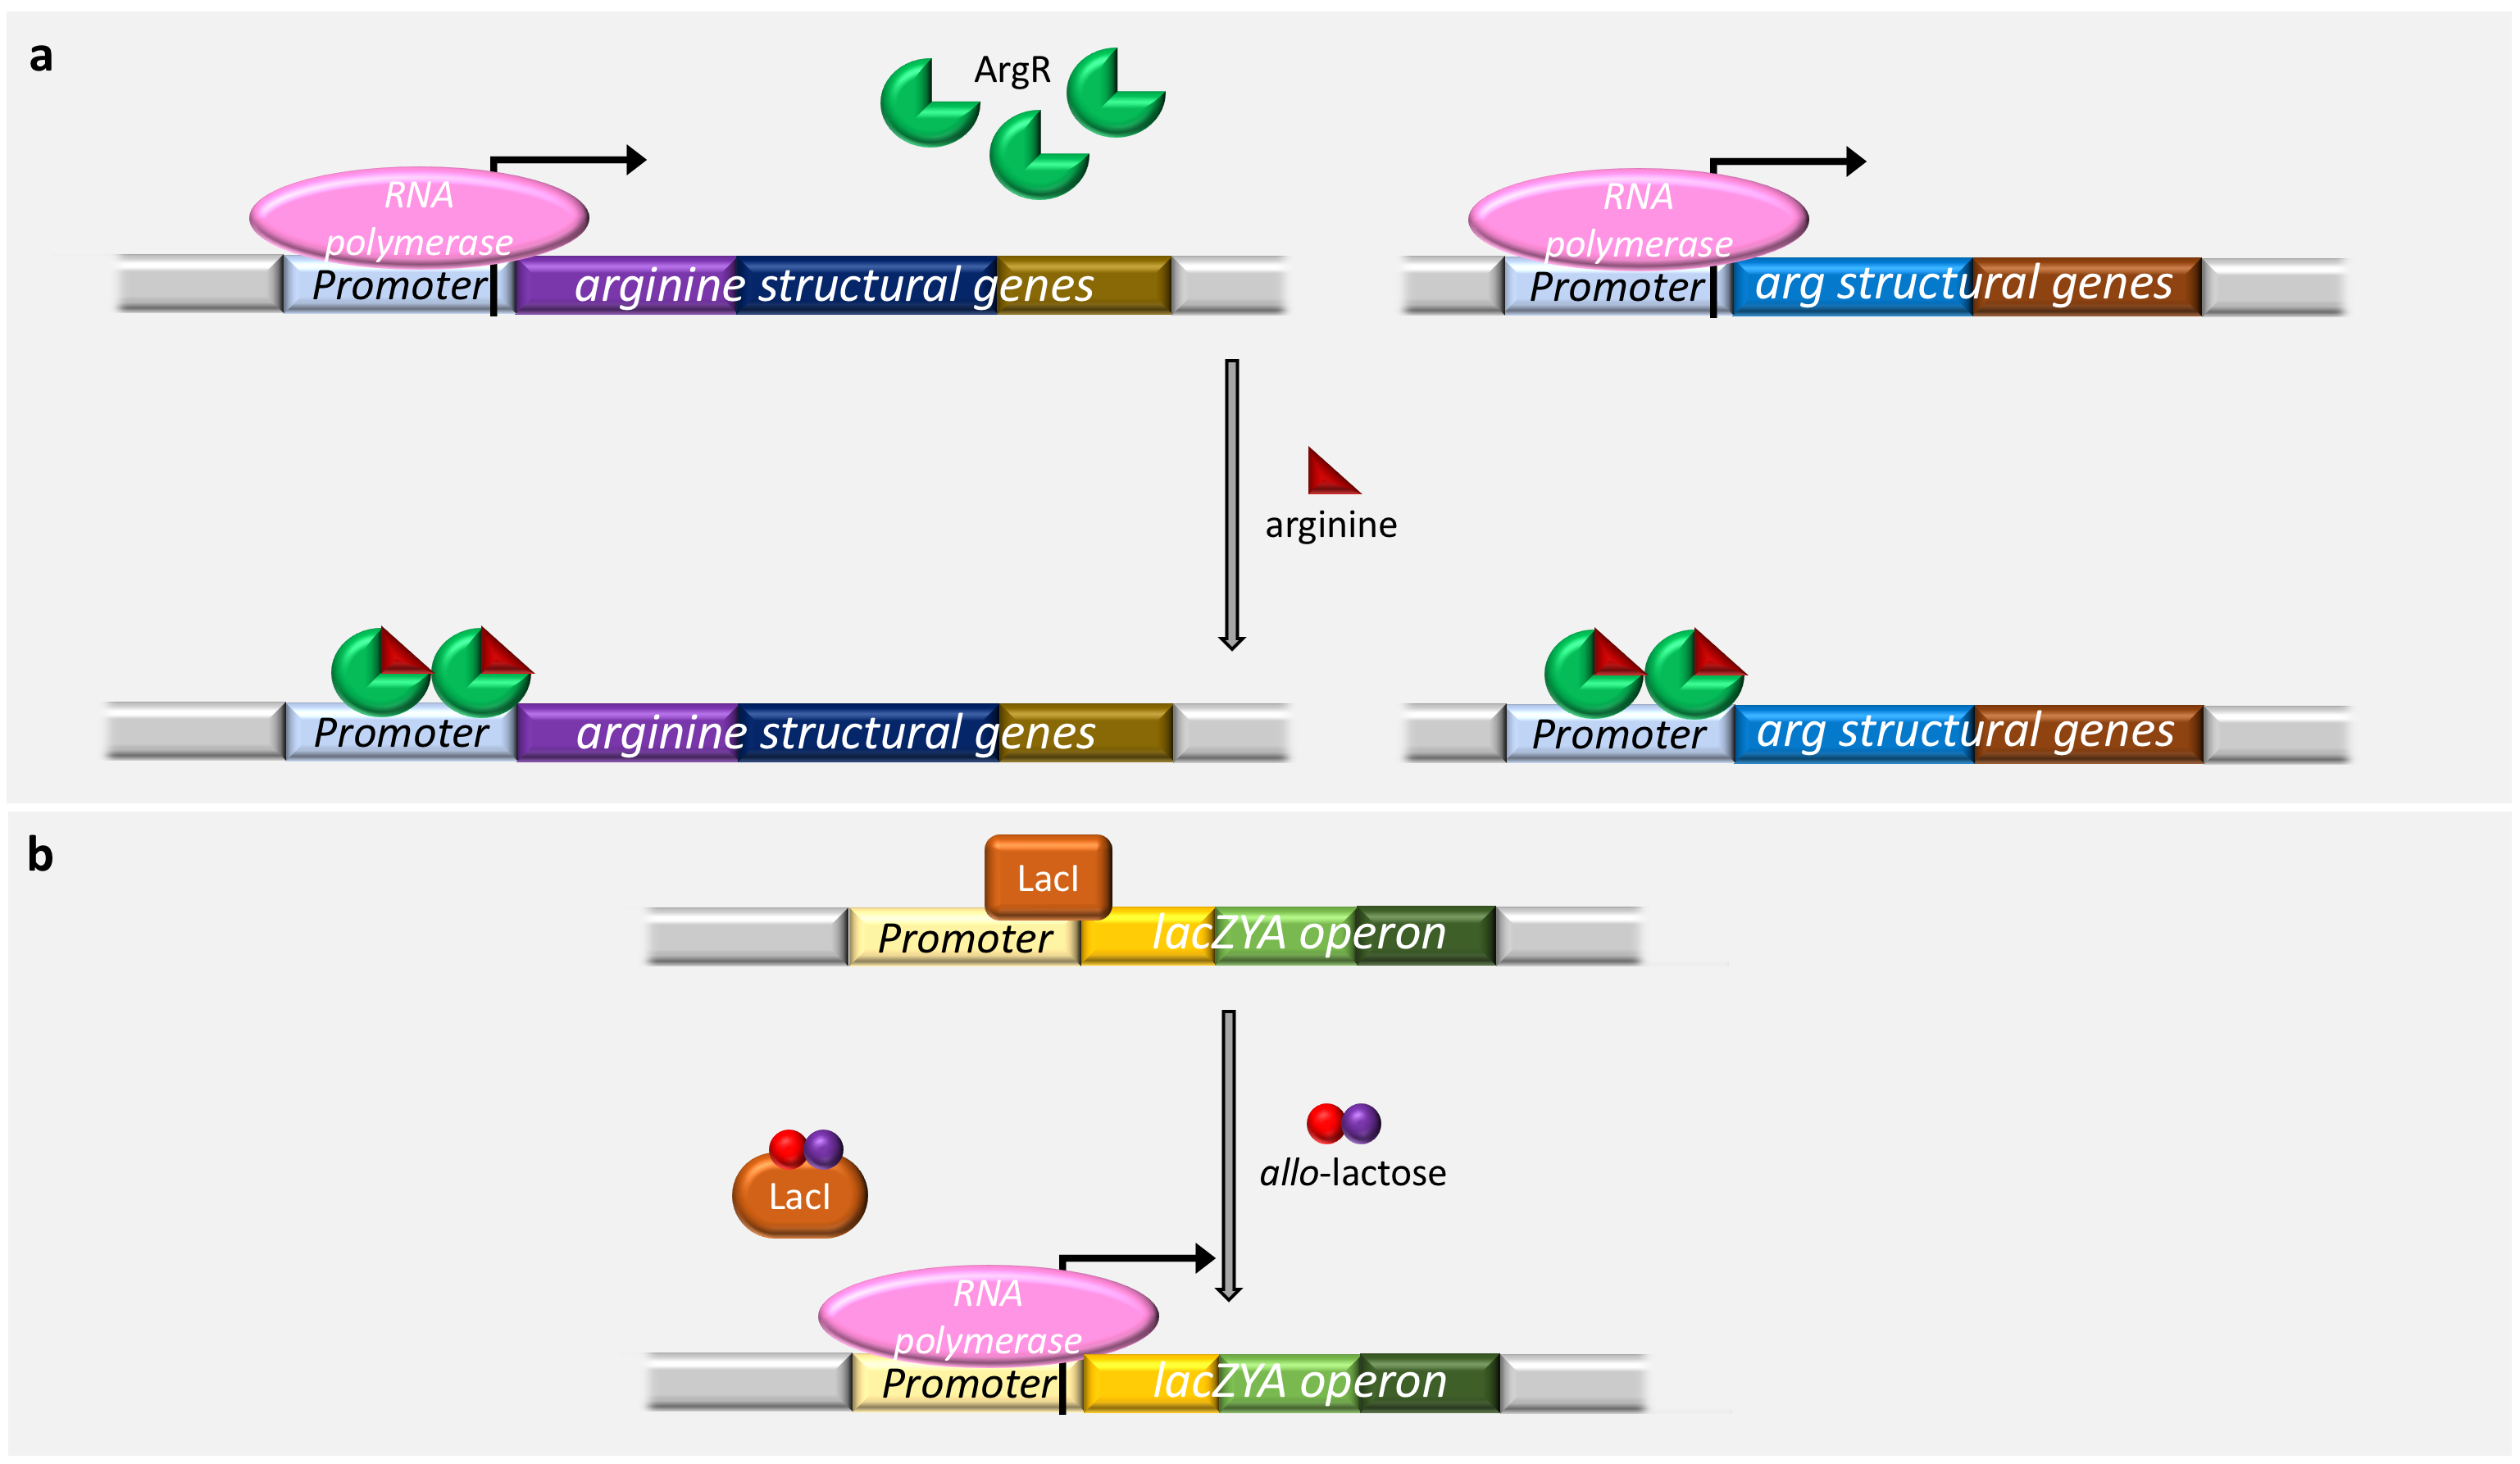
\includegraphics[scale=0.27]{text/Pictures/DirectSignaling.png}
	\caption{Scheme of direct signaling. \textbf{a} if \tax{lac} operon inducer (allolactose) is present it binds to LacI repressor and induces \tax{lac} operon transcription. \textbf{b} expression of arginine structural genes is co-repressed by arginine itself, because without it ArgR repressor cannot bind to DNA.}
	\label{dir}
\end{figure}

For other metabolic pathways things might work a different way, however.
Arginine, for instance, acts as a co-repressor of its own biosynthesis (Fig. \ref{dir}\textcolor{red}{b}).
This means that when a bacterium does not have enough of this amino acid available for protein production the transcription of arginine genes is active \cite{charlier2004biosynthesis, caldara2006arginine}.
On the other hand, when arginine is abundant in the culture medium and thus in the cell, there is no need to make more of it.
The cell has ArgR repressor present in cytosol but ArgR itself cannot bind to DNA and inhibit transcription in the arginine absence \cite{clark2005molecular, caldara2006arginine}.
However when there is plenty of arginine in the cell it binds to ArgR and as a co-repressor inhibits expression of arginine structural genes binding to an appropriate promoter \cite{charlier1992arginine, charlier2004biosynthesis, clark2005molecular}.

% Actually, you title the previous section as "Direct signalling pathways" Could you entitle this one as "Indirect signalling pathways" just for the nice contrast? Then two-component is just one example of indirect signalling.
\subsection{Two-component systems}
% so if you re-title the section, this would be "A classic example of indirect signalling is the two component system..."
% can you also put the word "transcription" somewhere in this section (keeps focus on txn as a common theme throughout).
A classic two-component system consists of a transmembrane sensory kinase which is autophosphorylated at its histidine residue after receiving physical or chemical signal from the environment (Fig. \ref{two}\textcolor{red}{a}).
To be able to phosphorylate itself the kinase requires ATP or other phosphate donor.
Next, the phosphorylated kinase transfers the phosphate group to its partner regulatory protein enabling its activity, most often DNA-binding \cite{lynch2012prioritization, gao2015temporal, cui2018novel}.
This protein receives the phosphate to its aspartate residue and might act as both gene repressor and/or activator.
Alternatively, the output of the two-component system can be a modification of biochemical activity of target proteins or RNAs instead or on the top of the change in gene expression \cite{shu2002antar, chambonnier2016hybrid}.

The described kinases and cognate regulatory proteins do not necessarily need to be separated units.
Proteins with histidine kinase domains connected to aspartate domains of DNA-binding proteins are known.
These hybrid systems are usually located in cell membrane with their sensory domains in periplasmic space (Fig. \ref{two}\textcolor{red}{b}) \cite{lynch2012prioritization, hirano2013regulon}.

\begin{figure}[h!]
  \centering
  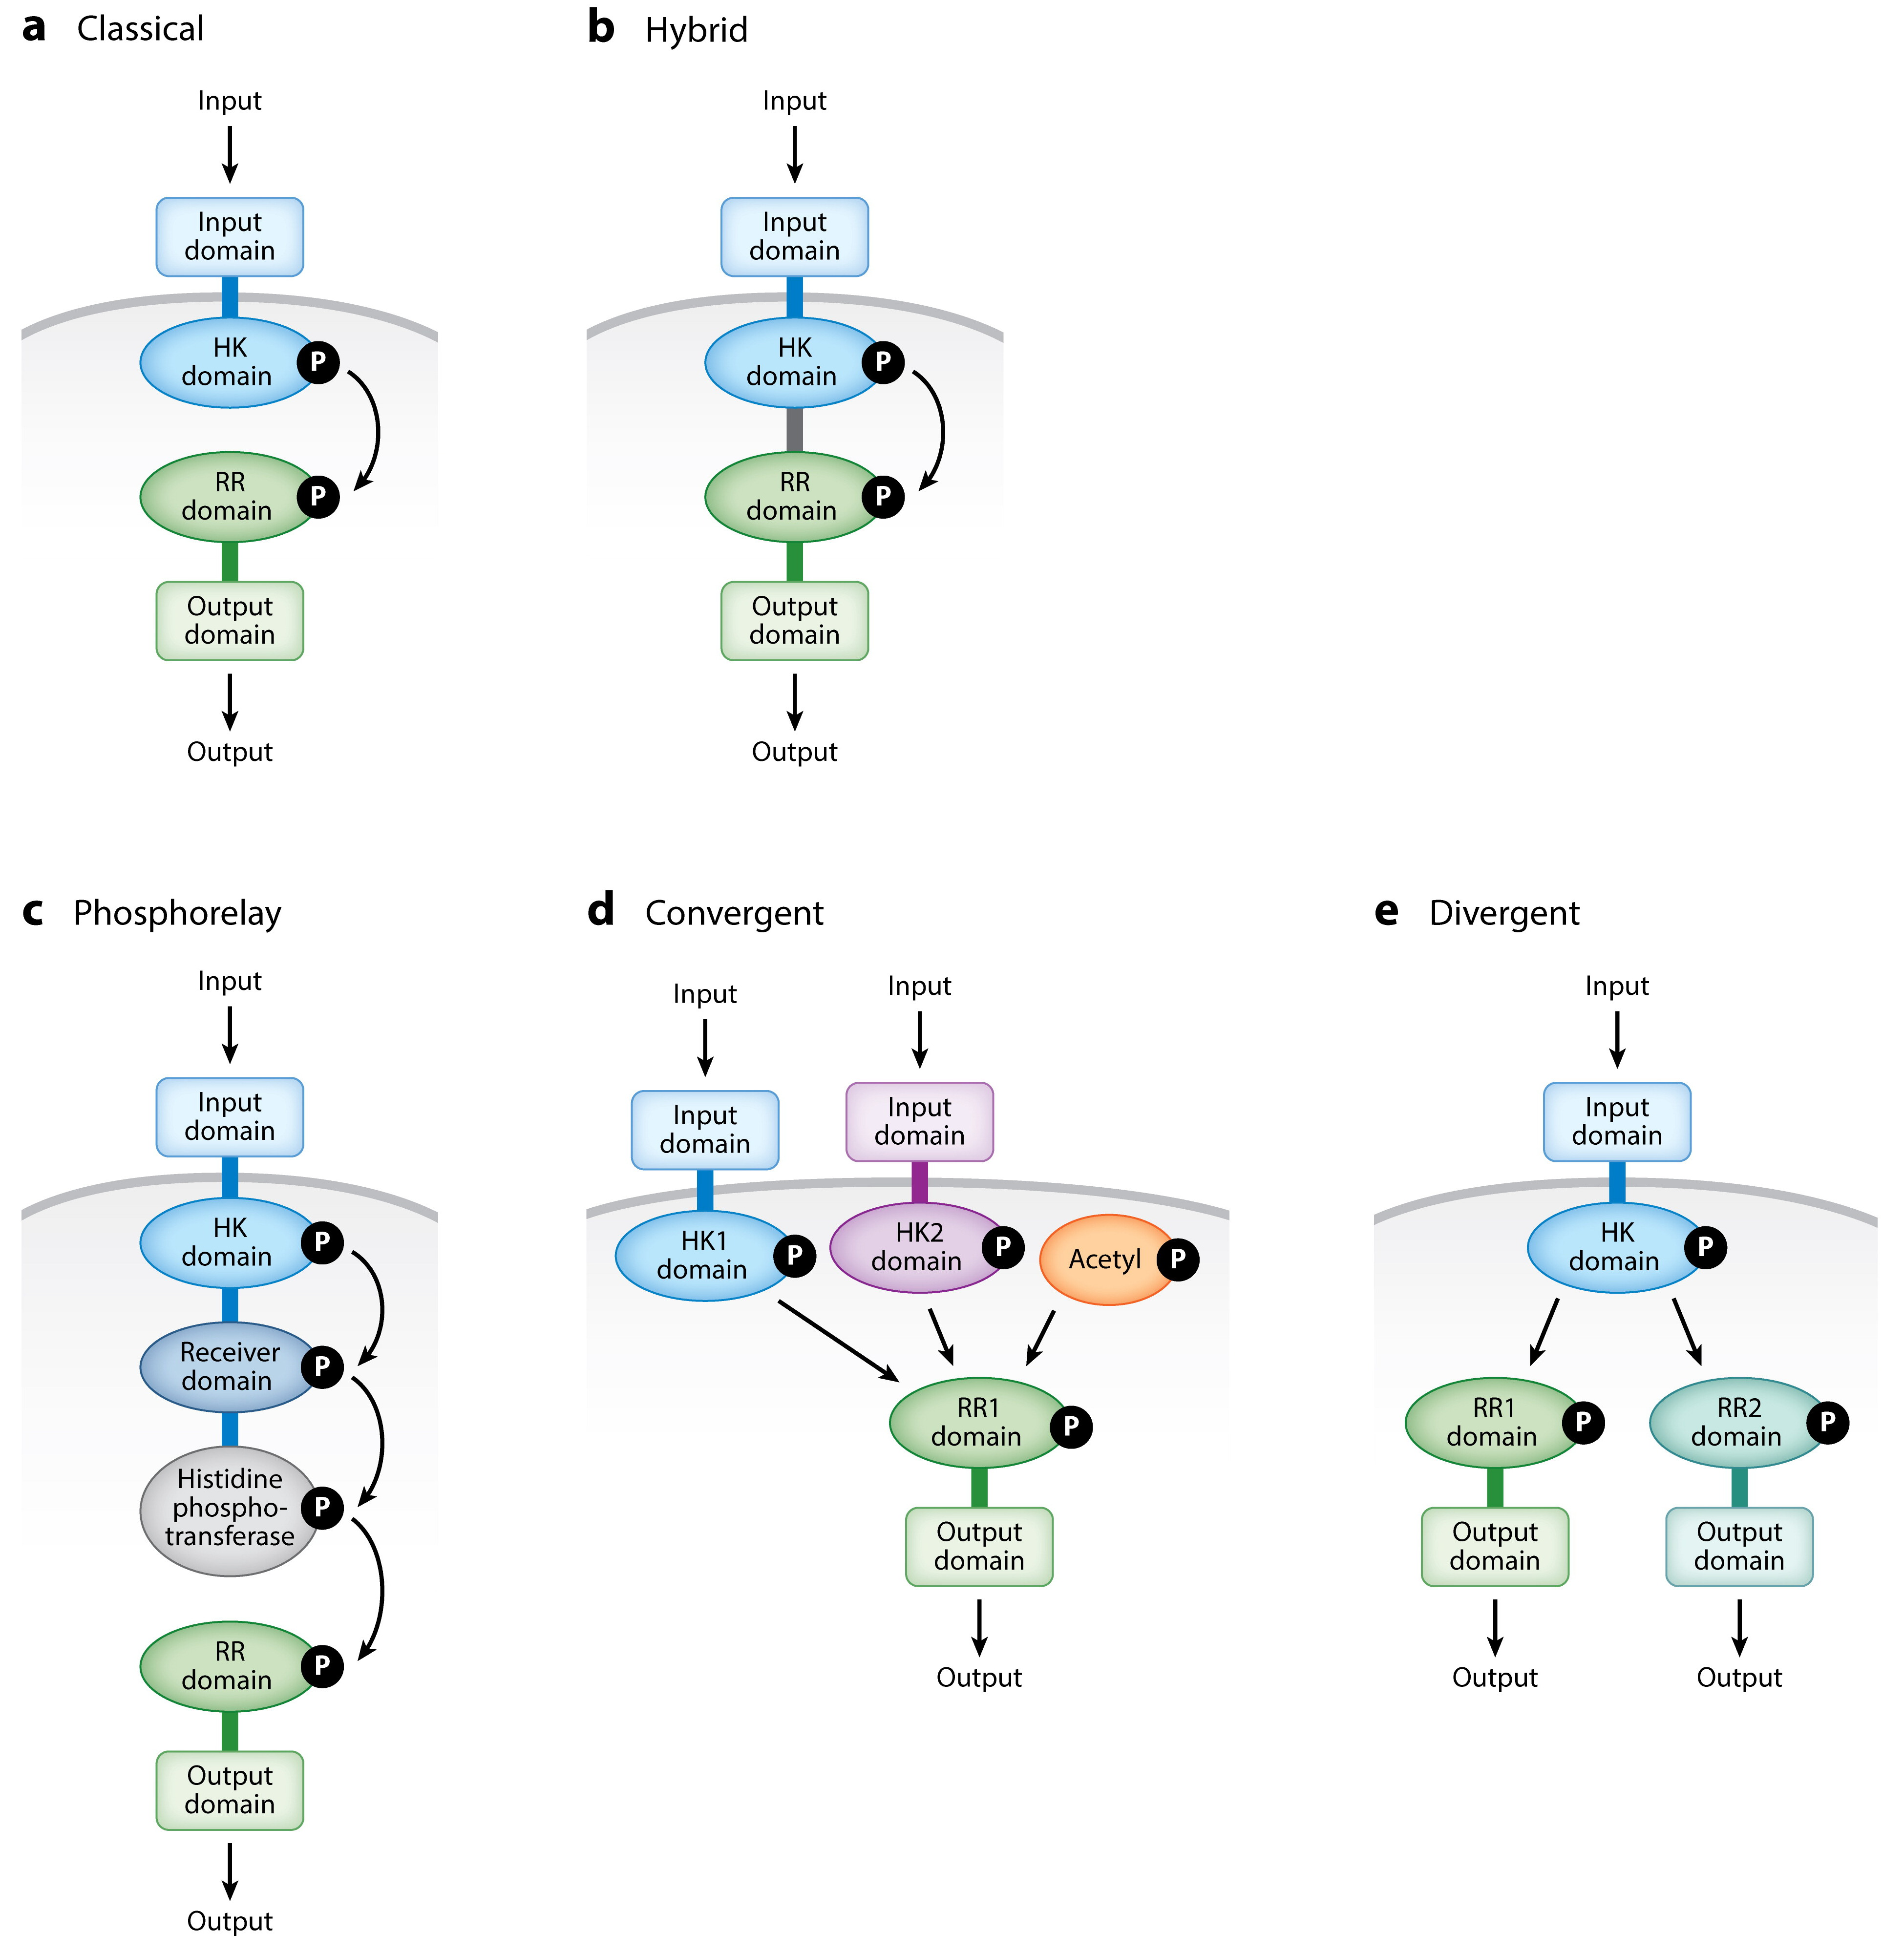
\includegraphics[scale=0.85]{text/Pictures/TwoComponent.jpeg}
	\caption{Two-component signaling pathways. \textbf{a} histidine kinase (HK) autophosphorylates in response to a signal and subsequently transfers the phosphate to a response regulator (RR) which generates output. \textbf{b} a hybrid system comprises both components (HK and RR) into a single protein. \textbf{c} in phosphorelay the phosphate is transferred multiple times before reaching its final RR. \textbf{d} some RR can be activated by several HK including metabolites such as acetyl phosphate. \textbf{e} one HK might phosphorylate multiple RR generating various outputs. (reproduced from \cite{groisman2016feedback})}
	\label{two}
\end{figure}

Another version of two-component system is phosphorelay (Fig. \ref{two}\textcolor{red}{c}).
In this case multiple steps of phosphate transfer occur before the final phosphorylation of target regulator.
Histidine domain of sensor protein serves here as a phosphate donor to an aspartate domain of the same or another protein.
From this domain the phosphate is further transferred to another histidine domain.
This can exist again within the same protein or as a separated one.
And finally, the aspartate domain of a DNA-binding regulator receives phosphate from the third domain in row.
These multiple steps allow an easier regulation by other signals as the phosphorelay can be silenced at any of the intermediate steps during the transmission \cite{perego2001pentapeptide, groisman2016feedback}.

Systems where a regulatory protein can be phosphorylated by different sensory units also occur.
And even phosphorylated metabolites might act as signal donors (Fig. \ref{two}\textcolor{red}{d}).
This results in similar outputs in response to various signals \cite{kaczmarczyk2014complex, chambonnier2016hybrid}.

Contrary, some cases require various response to a single signal, when multiple genes are affected.
A divergent signal transmission mediates this (Fig. \ref{two}\textcolor{red}{e}) as one sensory kinase is able to phosphorylate aspartate domains of different acceptor proteins \cite{mika2005two, groisman2016feedback}.
Moreover, all these variations of two-component system mentioned above combine in cells producing a complex sensory-response network \cite{kaczmarczyk2014complex, chambonnier2016hybrid}.

%%% FIRST I WROTE IT IN THIS SECTION, BUT IT'S MORE SUITABLE FOR SECTION ABOUT MEMORY I THINK:
%%% The way a bacterium reacts to a certain condition differs from a cell to cell depending on the cell cycle it is in, metabolic activity and remaining energy i.e. ATP present in the cell.
%%% However not all variations can be explained by that as even within these lets say homogeneous groups differences in behaviour are observed.
%%% More or less past events were shown to play a role in some of such instances, in others bet hedging strategy is likely the cause.


\section{Transcriptional networks}
%%% I SHOULD ADD SOMETHING HERE AND CHANGE ACCORDINGLY THE INTRO TO Bacterial gene regulation
% not sure what you mean here.


% After starting this section, I think you should put direct/indirect signalling *within* this section. Otherwise it makes it seem like they are different from the process of txn, which you descirbe here. So it's good if you start out with global changes (e.g. DNA accessiblilty, then move to more local (TFs and txn initiation)
\subsection{Bacterial gene regulation}
As mentioned above several ways of control of gene products take place in bacterial cells.
While control of protein activity helps to respond to quick environmental changes, translational regulation is a useful tool for controlling differential production of proteins coded within the same operon and thus transcribed on the same mRNA \cite{dar2018extensive}.
Transcriptional regulation on the other hand might be considered as the most economical as it inhibits the very synthesis of products which are not needed at the moment.
This saves resources and energy for synthesis of desired gene outputs.
The last mentioned type of regulation is delineated further in detail.

% sure, maltose is classic and might be an option. but you don't need your sections too long.
%%% A BIT MORE INFO ABOUT TRANSLATIONAL REGULATION IF NEEDED:
%%% Maltose operon \tax{malEFG} is one of them.
%%% Transmembrane proteins MalF and MalG are required in much lower amount than substrate-binding MalE protein for maltose ABC transporter function \cite{newbury1987differential}.
%%% Differential mRNA decay thus ensures there isn't too much of one protein (MalF and MalG) or too few of the other (MalE) even when transcribed together.

\subsubsection{DNA accessibility}
Having coding sequence and promoter of certain gene physically accessible for specific transcription regulation is one of the prerequisites of its expression.
Moreover differential physical access to DNA within a chromosome presents one of the explanations to observed variations in promoters activity based on their position in the chromosome \cite{bryant2014chromosome}.
Nucleoid associated proteins (NAPs) and supercoiling are general mechanisms affecting this accessibility.
NAPs' role in several cell processes such as replication, horizontal gene transfer or transcription regulation was shown \cite{dixon1984protein, kayoko1992histone, aznar2013hha}.
Here I mention principally their global influence of gene expression and respective DNA accessibility to other DNA-binding transcriptional factors and RNA polymerase.
NAPs in general have dual effect on transcription i.e. can act as both enhancers or silencers of genes.

H-NS is one of the most abundant nucleoid-associated proteins of \textit{E. coli} chromosome which occurs at all growth phases \cite{azam1999growth}.
Its expression is negatively autoregulated, but another NAP Fis acts as an activator of \tax{hns} gene \cite{ueguchi1993autoregulatory, falconi1996antagonistic}.
H-NS binds AT-rich DNA regions and forms polymers bridging distant DNA sequences  \cite{navarre2006selective, arold2010h}.
This leads to promoter silencing especially in cases when $\alpha$ subunit of RNA polymerase uses AT-rich sites to stabilize binding of the whole complex to the promoter \cite{singh2013h}.
However H-NS can compete with RNA polymerase and other transcriptional factors binding of AT-rich sites in general.
RNA polymerase might get even stuck in a DNA loop unable to elongate mRNA \cite{dame2002structural}.
Creation of such loops is the outcome of H-NS polymerization.
The silencing of affected promoters is not strict though as RNA polymerase sometimes bypasses this by association with an alternative $\sigma$ factors instead of conventional $\sigma^{70}$ \cite{grainger2008selective}.
Although H-NS is generally considered as global gene silencer an evidence of H-NS necessity for successful transcription initiation was published \cite{singh2013h}.

Fis protein similarly to H-NS prefers binding of AT-rich sites and is negatively autoregulated \cite{ball1992dramatic, stella2010shape}.
Fis's ability to affect gene expression in both positive and negative ways is better known \cite{choi2005effects, karambelkar2012silencing}.
Moreover it antagonizes H-NS silencing of some promoters \cite{falconi2001involvement}.
Even though Fis shares its binding preferences for AT-rich DNA with H-NS, it doesn't polymerase but bends the DNA sequence at the binding site \cite{hubner1989bent}.
This bending is essential for e.g. transcription initiation of ribosomal gene \tax{rrnB} \cite{gosink1993dna}.

These two NAPs described here belong among the ones which are most understood these days and don't represent an exhaustive outline of all bacterial NAPs.
Review from 2010 lists 14 additional bacterial NAPs \cite{dillon2010bacterial}, but even their list is not complete \cite{aznar2013hha}.

At the end of this block I'd like to mention supercoiling which also affects the access to the genetic code \cite{brahms1985activation}.
Overwinding (positive supercoiling) and underwinding (negative supercoiling) is generated during transcription when a transcription bubble forms \cite{wu1988transcription}.
This happens thanks to the helical structure of DNA.
Although some NAPs such as Fis and H-NS might affect the supercoiling levels \cite{ouafa2012nucleoid} topoisomerases take care of this process.
\tax{E. coli} possess two major topoisomerases - gyrase (topoisomerase II) and topoisomerase I.
The former releases positive the latter negative supercoiling \cite{wang1971interaction, gellert1976dna}.
If high levels of supercoiling are not released the access to the DNA reduces and even already initiated transcription is slowed down or terminated \cite{chong2014mechanism}.

\subsubsection{Regulation of transcription initiation}
Initiation of transcription is the very first step of gene expression and as that it is highly regulated.
The crucial step is RNA polymerase binding to the promoter sequence.
The rate of transcription initiation is proportional to the total amount of produced mRNA specifically if an early transcription termination doesn't occur \cite{kennell1977transcription, iyer1996absolute}.
Global control of this process based on physical access to DNA was described in the previous section.
Here I'm going to describe local regulation of this step involving transcription factors.
Activity of these factors corresponds to signals the cell acquires from internal or external environment as mentioned in the section dedicated to cellular responses.
Even though some factors control only one promoter, majority of at least \tax{E. coli} promoters is regulated by more of them \cite{karp2014ecocyc}.

% have you mentioned -10 / -35 yet? Should you explain what they are and what they're for?
\textbf{Repression} of promoters is often based on producing an obstacle in the place of -10 and -35 elements which blocks RNA polymerase binding to the promoter.
This is being achieved by various mechanisms.
The simplest one is repressor binding to the operator which overlaps one or both of those promoter elements \cite{brent1981mechanism} (Fig.~\ref{txn}\textcolor{red}{a}).
Other promoters have distant operators outside -10 and -35 elements, but bound repressors cluster creating a DNA loop which also constitutes a blockage \cite{semsey2004dna} (Fig.~\ref{txn}\textcolor{red}{a}).
A more complex and indirect way of repression is by inhibiting activators (described below) - i.e. repressors acting as anti-activators \cite{sogaard1993protein}.
Because some promoters require activation for the transcription initiation, anti-activation might be sufficient for complete repression (Fig.~\ref{txn}\textcolor{red}{a}).

Activity of certain promoters can be controlled gradually.
Such promoter sequences have arrays of operators and the amount of bound repressors affects the strength of the repression.
Some promoters are also recognized by more than one kind of repressor which usually don't affect each other \cite{el2009repression}.

\begin{figure}[ht!]
  \centering
  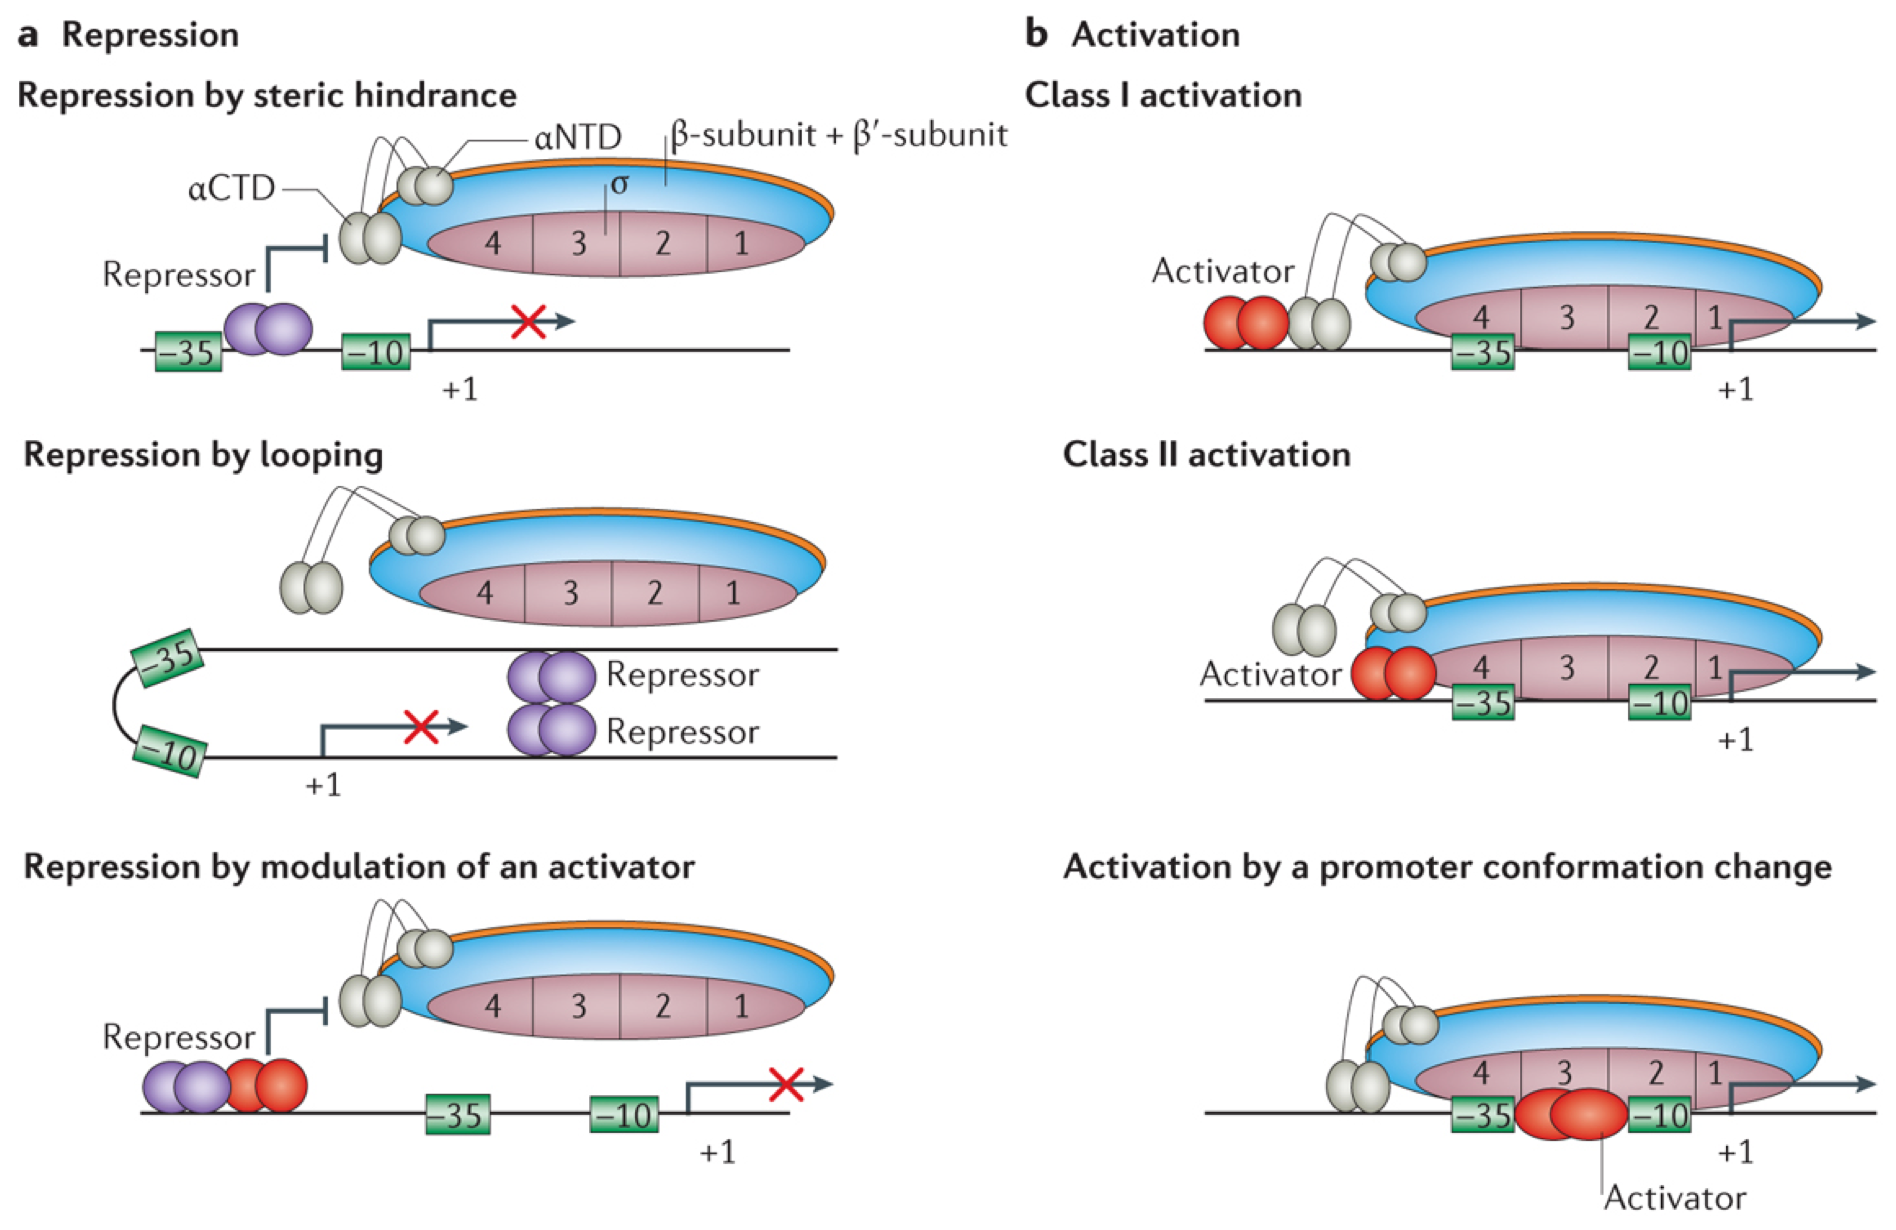
\includegraphics[scale=0.4]{text/Pictures/TxnInitRegulation.png}
	\caption{Regulation of transcription initiation by repressors and activators. (reproduced from \cite{browning2016local})}
	\label{txn}
\end{figure}

\textbf{Activation}, on the other hand, enables particular gene transcription or increases strength of RNA polymerase binding to the promoter.
Similar to the repression, some activators interact directly with RNA polymerase but other act indirectly as anti-repressors most often by releasing and preventing repressor binding to the operator \cite{frederix2011co}.
Besides affecting sequence specific repressors, some indirect activators affect also binding of NAPs, thus opening an access for RNA polymerase to the promoter sequence \cite{santana2001transcriptional}.
Direct activators mostly facilitate the very interaction of RNA polymerase and promoter.
Three mechanisms of direct activation are usually described: class I activation, class II activation and activation by conformational change.

Class I activators bind upstream of -35 element and interact with $\alpha$ subunit of RNA polymerase \cite{ushida1990helical} (Fig.~\ref{txn}\textcolor{red}{b}).
Operators of class II activators in turn overlap with -35 promoter element and the activators interact with given $\sigma$ factor of RNA polymerase \cite{igarashi1991functional} (Fig.~\ref{txn}\textcolor{red}{b}).
Moreover bound class II activator prevents binding of the RNA polymerase $\alpha$ subunit to the preferred position right upstream of -35 element.
Class I and class II activation thus can occur simultaneously on the same promoter when two different activators are required to trigger the transcription \cite{lloyd2002requirement}.

The last classical activation mechanism causes a conformational change of the sequence between -10 and -35 elements.
RNA polymerase binding to these promoters without activator is weakened or impaired due to inappropriate distance between -10 and -35 elements.
And this is also where the operators of such activators are located (Fig.~\ref{txn}\textcolor{red}{b}).
A bound activator then brings the elements into the optimal position for RNA polymerase recruitment \cite{heldwein2001crystal}.

All activation mechanisms mentioned above just enable RNA polymerase binding strong enough for an efficient transcription initiation.
Other kind of activation of transcription initiation is not even required for most RNA polymerase holoenzymes.
However, RNA polymerase containing $\sigma^{54}$ factor is unable to unwind promoter DNA to begin transcribe.
This is facilitated by enhancer binding proteins (EBPs) which interact with the $\sigma^{54}$ factor \cite{morett1989vivo, cannon2000dna}.
Nevertheless, EBPs bind upstream of the promoter elements, so to get in contact with the $\sigma^{54}$ factor a loop has to be produced.
Production of this loop is known to be mediated by nucleoid associated protein IHF which as well as other NAPs plays a role in DNA accessibility \cite{de1991upstream, sze2001vivo}.

\subsubsection{Regulation of mRNA elongation and transcription termination}
After a successful transcription initiation the elongation of mRNA follows until termination comes to place.
Even though the main transcription regulation occurs at the level of transcription initiation, elongation and termination can be also modulated, ranging from repression of elongation \cite{monsalve1996protein}, through elongation pausing and backtracking \cite{mustaev2017transcription} to transcription attenuation and anti-termination \cite{naville2009transcription}.

To the end of the section about transcription regulation it is good to point out the complexity of the whole process.
Even when both global and specific regulation of transcription initiation permit transcript production the gene expression is still regulated further downstream e.g. during mRNA elongation or translation.
Moreover one transcription factor can regulate multiple genes as well as being co-regulated by several factors including itself.
Regulation of gene expression thus exhibit a huge network of mutually controlled outputs based on the information acquired by a cell.

\subsection{Regulatory kinetics}
For better understanding the whole transcription network regulation, it is important to look at the speed of different regulatory circuits as well.
This is usually characterised by a rise-time (or response time), i.e. time when the concentration of a gene product reaches its half maximal concentration after gene induction.

\subsubsection{Promoter strength and protein lifetime}
Naturally the more easily and often RNA polymerase binds effectively to a promoter the more of an appropriate protein is produced at the time.
The strength of the promoter is given by its nucleotide sequence and binding of transcription factors increases or decreases RNA polymerase affinity to it.
On the other side of this equilibrium is degradation of the product, as its stability in certain conditions determines its lifetime.
A functional protein is also diluted during cell division, which further reduces its amount per cell.

\subsubsection{Transcriptional network motifs}
% some figures / cartoons here? Could be useful. This seciton is good otherwise.
As an additional fine tuning of transcriptional response speed the simple network motifs themselves can be considered.
% the "same" concentration == equilibrium concentration?
It has been shown that a negatively autoregulated gene reaches the same concentration much faster than if it is not autoregulated \cite{rosenfeld2002negative}.
In other words negative feedback loop shortens the product rise-time.
It also reduces the variability in product concentration maintaining it in optimal concentration limits \cite{becskei2000engineering}.
This enables the cell to use stronger promoters for proteins needed in a short time but at low concentration without overshoots and risks of protein toxicity.

Positive autoregulation exhibits right the opposite traits.
Slower and noisier initial response to gene activation is observed in case of positive feedback loops compared to no feedback systems \cite{maeda2006regulatory, sayut2007noise}.
Although it takes longer for the cell to reach certain level of desired protein, this motif allows to react to much lower concentrations of signal.
Moreover, both graded and hysteretic expression can be observed in positively autoregulated genes \cite{maeda2006regulatory}.
%%% IS THIS ENOUGH TO MENTION DIFFERENCE IN GRADED AND BINARY RESPONSE IN HERE OR DO YOU WANT ME TO EXPAND IT MORE IN e.g. A SEPARATE PARAGRAPH

Next common regulatory motifs in \tax{E. coli} are feed-forward loops (FFLs).
% the grammar in the next sentence is a bit off.
% there's a lot of abbreviations (e.g. FFL) and X factors piling up here. Can you change "X" to something mroe reader friendly? Not sure what / how...
By FFL is meant a regulatory circuit when a transcription factor X regulates other transcription factor Y and both (X and Y) regulate a gene or operon Z.
There is further distinction between coherent and incoherent FFL.
When the regulation of Z by factor X has the same sign (positive or negative) as regulation of Z by X through Y we talk about coherent FFL.
If the signs are opposite the FFL is considered incoherent \cite{shen2002network}.
It has been predicted that coherent FFLs cause sign-sensitive delays in regulatory kinetics and incoherent FFLs should act as sign-sensitive accelelators and exhibit transient pulses of expression \cite{mangan2003structure}.
The most abundant schemes were later experimentally confirmed.
%%% IT'D BE GOOD TO HAVE PICTURE TO SUPPORT THE LAST SENTECE OF THE PARAGRAPH.

In coherent FFL type 1 factor X activates factor Y expression and both X and Y positively regulate transcription of Z \cite{mangan2003structure}.
There are two possible ways of induction of Z expression in this system.
First, both factors X and Y has to bind Z promoter to trigger transcription - AND-gate logic (AND-FFL).
Or only one of both is sufficient to activate Z gene - OR-gate logic (OR-FFL).
The AND-FFL was shown to delay full gene expression compared to non-FFL system \cite{mangan2003coherent}, while no delay was observed in the inverse (ON to OFF) transition.
To test OR-FFL a system where X and Y act in additive manner to activate Z was used and termed as SUM-FFL \cite{kalir2005coherent}.
This motif behaves right the opposite way than AND-FFL.
Transition from OFF to ON shows no delays.
But when factor X was deactivated the ON to OFF step was considerably delayed in comparison with strain with deleted gene for factor Y.
The former motif (AND-FFL) thus prevents Z expression when concentration of X fluctuates close to a threshold, while the latter circuit (SUM-FFL) enables continuous production of Z even if X concentration drops below a threshold for a while.

From incoherent FFL motifs the type 1 is predominant in \tax{E. coli} transcriptional network.
Factor X here positively regulates both Y and Z, however factor Y acts as an inhibitor of Z gene.
The model predicted this incoherent FFL to speed up transcriptional responses, but weak pulse-generating power was expected \cite{mangan2003structure}.
Nevertheless this motif was used to create effective pulsers \cite{basu2004spatiotemporal}.
Later the acceleration trait was experimentally confirmed as well despite the fact that other motifs contribute to the used regulatory system \cite{mangan2006incoherent}.
This suggests that the motifs' fundamental functions are preserved even when combined with other motifs.
Overall this type of regulation similarly to negative feedback loop shortens the rise-time, but unlike the negative feedback doesn't avoid overshoots rather the opposite.
The overshoot is seen as a pulse of high gene Z expression which is subsequently inhibited by factor Y, but not necessarily back to the basal level.


\section{Epigenetics in bacteria}
Epigenetics is understood as a heritable change in gene expression without simultaneous changes in DNA primary sequence.
Some studies has shown that cells with the same genetic background might react differently or at a different rate to the same stimulus based on their and their ancestors recent experience \cite{mathis2017asymmetric, ronin2017long}.
Such ability is advantageous especially if the change in the conditions is predictable and repeats periodically.

\subsection{Mechanisms of bacterial memory}
Various epigenetic mechanisms such as histone modifications, genomic imprinting or RNA associated silencing are well studied in eukaryotes \cite{durso2014mechanisms}.
In bacterial domain DNA methylation by methyltransferases is mostly mentioned, although positive and double negative feedback loops play their role as well especially in terms of population bistability \cite{casadesus2006epigenetic, casadesus2013programmed, adhikari2016dna}.

% 2018.06.28
% Eventually, go into way more detail here, as this will end up as a full section on lac. But if you are leaving this as a brief intro to positive, negative, double negative, that's fine. You might also start with sensing/reaction and then move to epigenetics. This is a reasonable ref I think *An introduction to systems biology: design principles of biological circuits*, although you always have to be a little careful with Uri Alon's take on things, sometimes it's a bit too facile.
\subsubsection{Feedback loops}
System where a product is able to affect positively or negatively its own production is called a feedback loop.
The influence of the output on itself might be direct or indirect if multiple effectors are involved.
Feedback loops are quite common in bacterial gene regulation and can lead to epigenetic switches \cite{smits2006phenotypic, veening2008bistability}.
Positive feedback loop and double negative feedback loop are known to play a role in memory of prokaryotes so far and are characterized in detail below.

\textbf{Positive feedback loop} is the first described example of bacterial epigenetics.
It was shown already in 1957 that \tax{E. coli} sub-population primed by high concentration of lactose analogue TMG is able to maintain \tax{lac} operon fully induced even in low non-inducible TMG concentrations \cite{novick1957enzyme}.
While if the same bacteria are exposed to the low non-inducible TMG concentration without priming the \tax{lac} operon remains repressed by LacI.
The mechanism behind this resides in different levels of $\beta$-galactoside permease (LacY) in TMG induced and naive cells.
Induced population has high level of the permease present in membrane as \tax{lacY} gene expression is activated by high TMG concentrations.
This state is preserved in a sub-population of induced cells after transfer into low TMG concentration as the abundant permease is able to maintain intracellular TMG level high enough to avoid LacI repression.
Thus the high level of permease leads to high intracellular TMG concentration which in turn acts as permease transcription activator.
On the other side naive cells have very small amounts of LacY if any thus they are not able to obtain TMG from the solution to activate \tax{lac} operon expression \cite{smits2006phenotypic, casadesus2013programmed}.

\begin{figure}[h!]
  \centering
  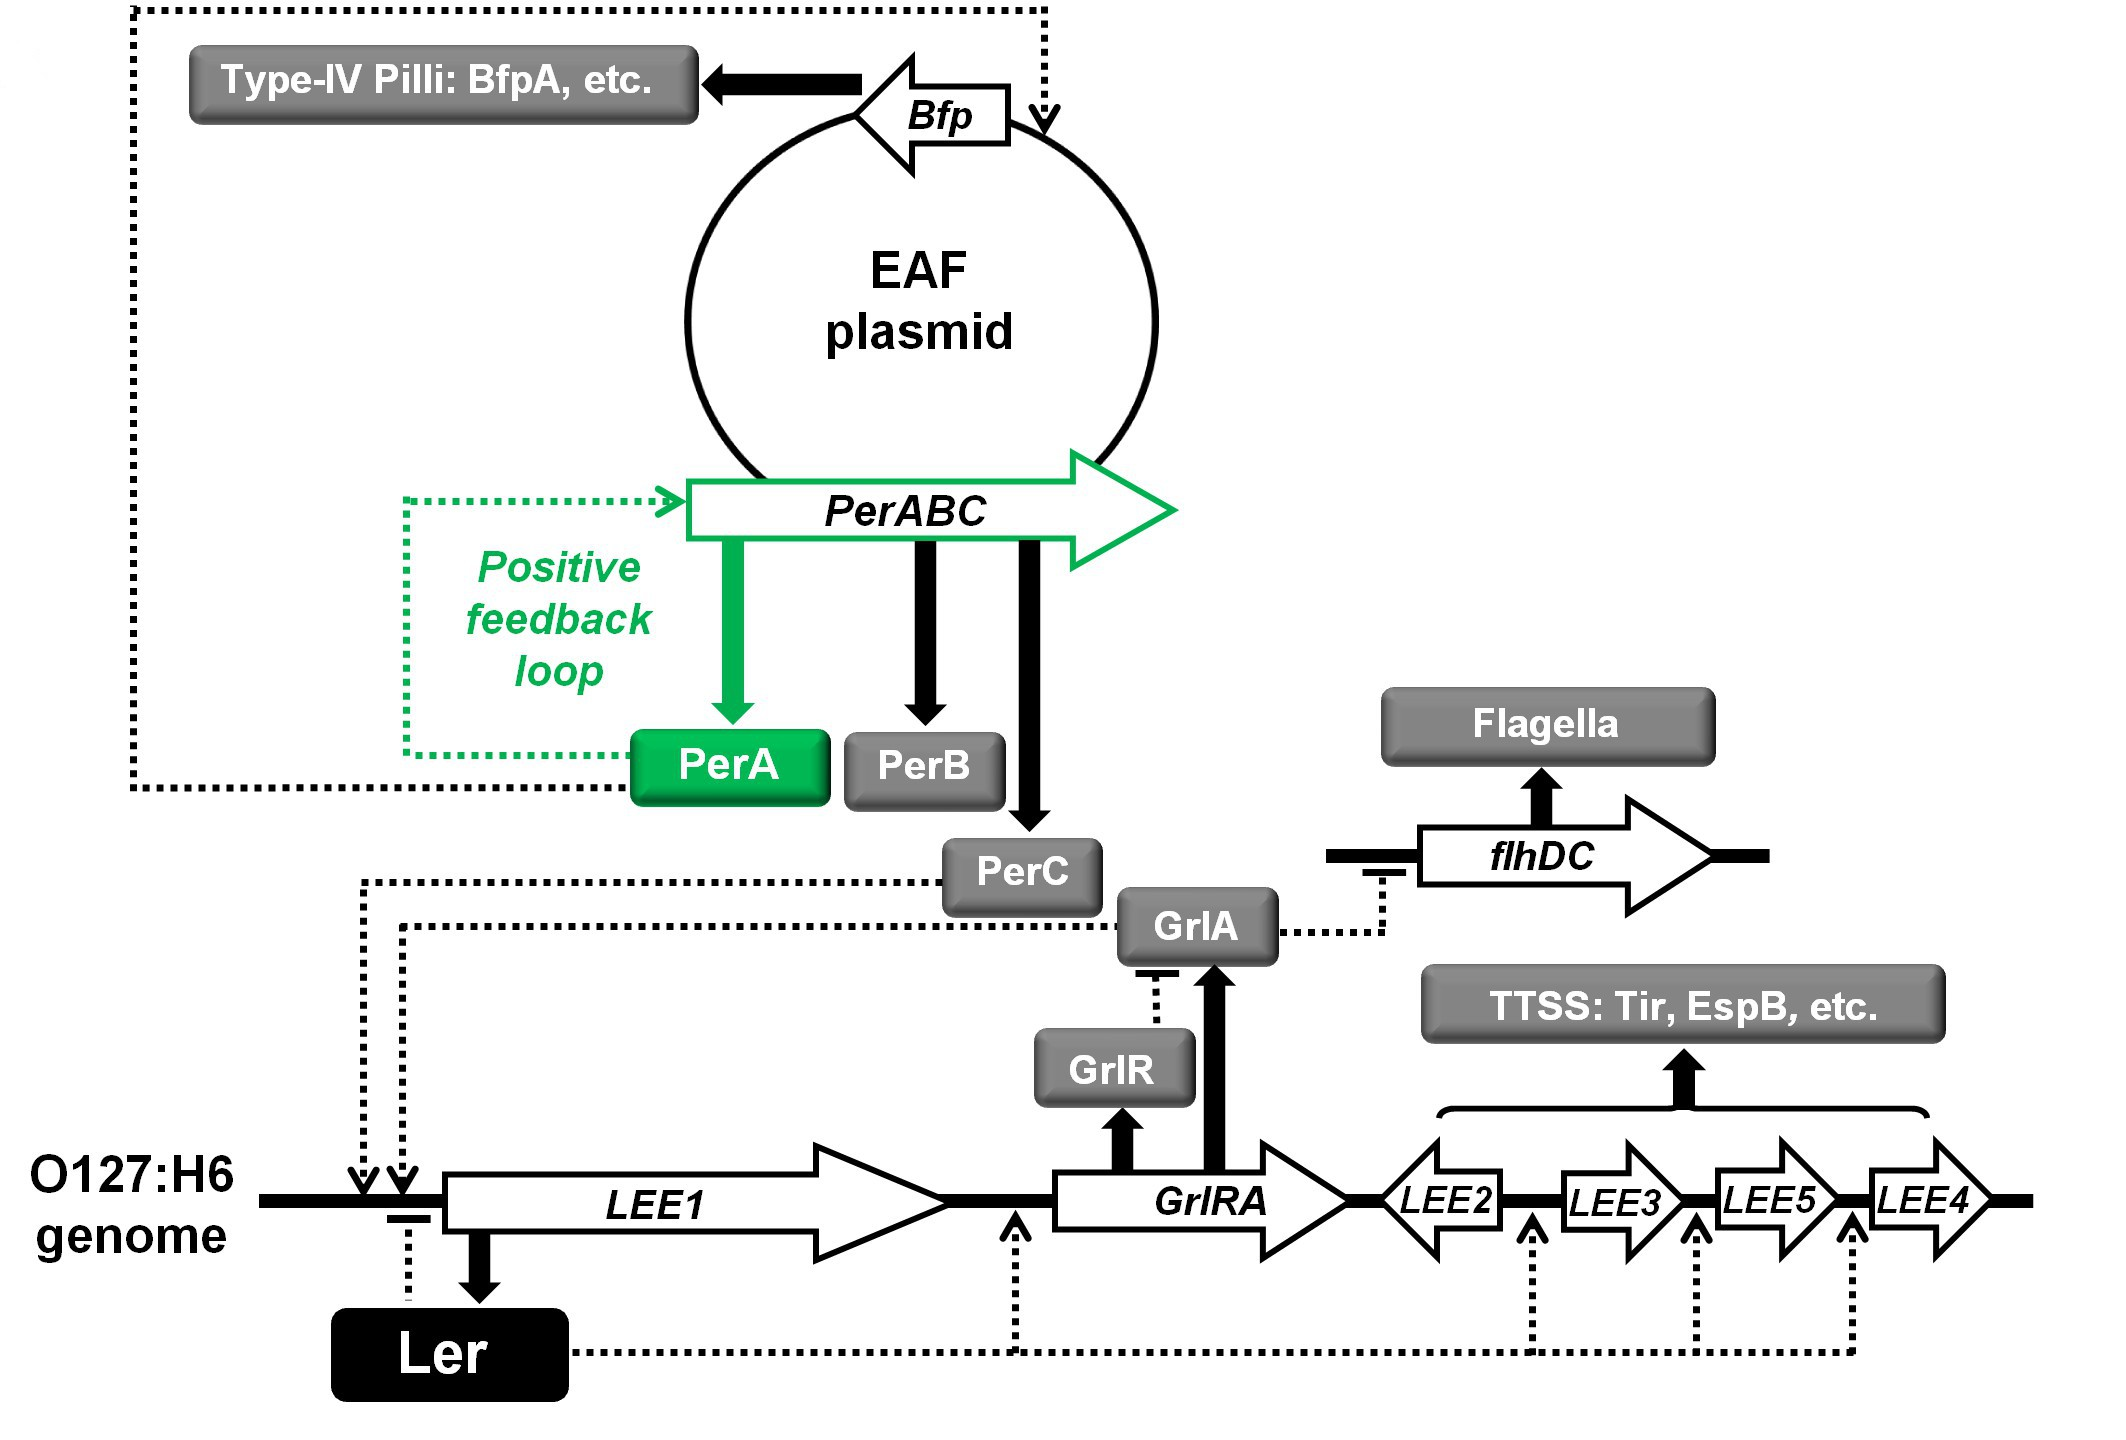
\includegraphics[scale=0.2]{text/Pictures/perOperonRegulation.jpg}
	\caption{Scheme of EPEC virulence regulation. PerA positivelly autoregulates \tax{perABC} operon and the triggers expression of type IV pili. PerC activates transcription of Ler which is the main regulator of T3SS secretion system machinery. (reproduced from \cite{ronin2017long})}
	\label{per}
\end{figure}

Another nice example of a long-term virulence epigenetic switch mediated by a positive feedback loop was published last year.
Enteropathogenic \tax{E. coli} (EPEC) coexists in two, non-virulent and hyper-virulent, sub-populations during growth \cite{ronin2017long}.
This bimodality was first observed  using ScanLag \cite{levin2014scanlag} as a difference in growth rates of the two groups resulting in BIG and SMALL colony morphotypes, for early and late appearing colonies, respectively.
At transcription level it is a change in \tax{per} operon expression (located on EAF plasmid) and \tax{per} regulated genes.
EPEC cultivation in virulence-activating conditions gives rise to \tax{per}-ON hyper-virulent aggregative sub-population (SMALL phenotype) reaching nearly 100\% \cite{ronin2017long}.
Interestingly this high ratio of \tax{per}-ON vs \tax{per}-OFF cells remains for many generations even after transferring the culture back into non-activating conditions, although naive EPEC culture contains only a minority of \tax{per}-ON cells.
Transition back from \tax{per}-ON to \tax{per}-OFF phase is achieved when cells are grown up to stationary phase.
The long-term stability of \tax{per}-ON state relies on a positive feedback of PerA which acts as an activator of its own gene beside \tax{perB} and \tax{perC} in the \tax{per} operon (Fig.~\ref{per}) \cite{ibarra2003identification, ronin2017long}.
%%% More examples of positive feedback to add???

As an illustration of \textbf{double negative feedback loop} in epigenetic regulation a switch between lytic and lysogenic cycle of \tax{E. coli} phage $\lambda$ is often described \cite{smits2006phenotypic, casadesus2013programmed}.
After inserting its DNA the virus cycle might undergo two different ways - i.e. either replicate producing a lot of new phages and heading for bacterial lysis or integrate its own DNA into the bacterial chromosome and persist there within a lysogeny.
The fate of the phage lies in two repressors, CI and Cro, each repressing transcription of the other \cite{eisen1970regulation, neubauer1970immunity}.
Besides CI inhibits phage propagation genes and activates its own transcription.
However, both CI and Cro are produced since the beginning of the infection.
If the level of CI reaches a certain threshold and outcompetes Cro, whose activity is suppressed, the phage enters a lysogenic cycle staying dormant in the cell thanks to CI-\tax{cI} positive feedback loop.
Otherwise Cro levels rise further inhibiting CI production and establishing phage proliferation with subsequent cell lysis \cite{svenningsen2005role}.
It should be noted that although it is not predictable whether the phage enters lytic or lysogenic cycle, the ratio of lysed/lysogenized cells depends on bacterial physiologic situation and other environmental factors as well.
Interestingly, Toman et al. used the CI-Cro system for epigenetic reuglation of \tax{gal} operon in \tax{E. coli} \cite{toman1985system}.
%%% it's not epigenetics in E. coli, but in the phage lambda! (except for the engineered system by Toman et al.)

%%%As the CI-Cro regulation is a phage system, the first evidence of bacterial epigenetics driven by a double negative feedback loop was published just 3 years ago.

%%% detection of double negative feedback loop originating in bacteria?
%%% double negative feedback detected in "A Novel Feedback Loop That Controls Bimodal Expression of Genetic Competence" which talks about cell competence
%%% there is no direct evidence for epigenetics playing role in it, however paper "Agent-based modeling of competence phenotype switching in Bacillus subtilis" suggests it might be so according to their model
%%% especially when in similar case - bacillus sporulation is it proven in: "Bet-hedging and epigenetic inheritance in bacterial cell development"

\subsubsection{DNA methylation by orphan methyltransferases}
% in my opinion you can shrink this section a bit.
% one thing to note is that you have gone back and forth between very general topics (the toplogy of regulation networks), to more specific mechanisms (regulating txn via TFs), to very specific mechanisms (dam / dcm). Don't dive too deep. Deep dives into very particular cellular mechanisms can be for later (e.g. if you end up doing a lot fo work on one type of mechanism).

Orphan methyltransferases (MTs) were initially studied within restriction-modification system as a bacterial defence against phages, although Dam's ability to alter some gene expression was already described in mid-80s \cite{sternberg1985evidence, bickle1993biology}.
As orphan MTs lack their cognate restriction endonucleases their role in bacterial cells is not as a primitive immune system, but among others can act as a transcription regulators.
I describe the epigenetic mechanisms of Dam in detail below as the MT whose relationship to cell memory is most understood.
Some authors consider the change in expression of certain genes in \tax{Caulobacter crescentus} which is associated with an orphan MT called CcrM to be epigenetic as well \cite{casadesus2006epigenetic, adhikari2016dna}.
However I do not include it here as these transcriptional changes are not heritable and occur only during a part of a cell cycle.
Other \tax{E. coli} orhan MTs are mentioned briefly as well although none of them is known to play a role in epigenetics so far.

\textbf{Dam}, one of two first orphan MTs described in \tax{E. coli}, methylates adenine in 5'-GATC-3' sequences to N$^6$-methyladenine (6mA) \cite{marinus1973isolation}.
Its homologs were found in some bacteriophages as well as in other \tax{Gammaproteobacteria}, however many of bacterial DNA adenine methylases are associated with restriction endonucleases \cite{low2001roles, casadesus2006epigenetic, bochow2012bacteriophage}.
On the other hand strains having an orphan DNA adenine methylase can be characterized by presence of SeqA and MutH, overrepresentation of GATC sites in \tax{oriC}, genes close to it and in the \tax{dnaA} promoter \cite{sobetzko2016distamo}.
For most of the DNA both strands of chromosome are fully methylated throughout the cell cycle if Dam is present.
Of course, one of the exceptions is a short time hemimethylation of a leading strand and Okazaki fragments right after their synthesis during replication.
Both strands lack GATC methylation in \tax{dam} mutants, moreover higher mutation rate, uncoordinated replication initiation or loss of virulence were observed as well.
Interestingly for some species e.g. \tax{Vibrio cholerae} the presence of an orphan DNA adenine methylase is vital, whereas it is non-essential for other, such as \tax{E. coli} \cite{casadesus2006epigenetic, casadesus2013programmed, adhikari2016dna}.

As implied above several GATC sites escape Dam methylation.
This happens if another regulatory protein recognises a specific DNA biding site which overlaps GATC sequence and thus competes with Dam for it \cite{correnti2002dam}.
Such mechanism leading to epigenetic switch is well characterized in synthesis of \tax{pap} pili in uropathogenic \tax{E. coli} (UPEC) \cite{peterson2008competitive}.
The regulatory sequence of the \tax{pap} operon contains two sets of Lrp binding sites 1-3 and 4-6.
In both of them GATC sequence is present, GATC$^{prox}$ within site 2 and GATC$^{dist}$ within site 5 (Fig.~\ref{pap}) \cite{blyn1990regulation}.

% This is good. Maybe label the lrp sites as you refer to them in the text?
\begin{figure}[h!]
  \centering
  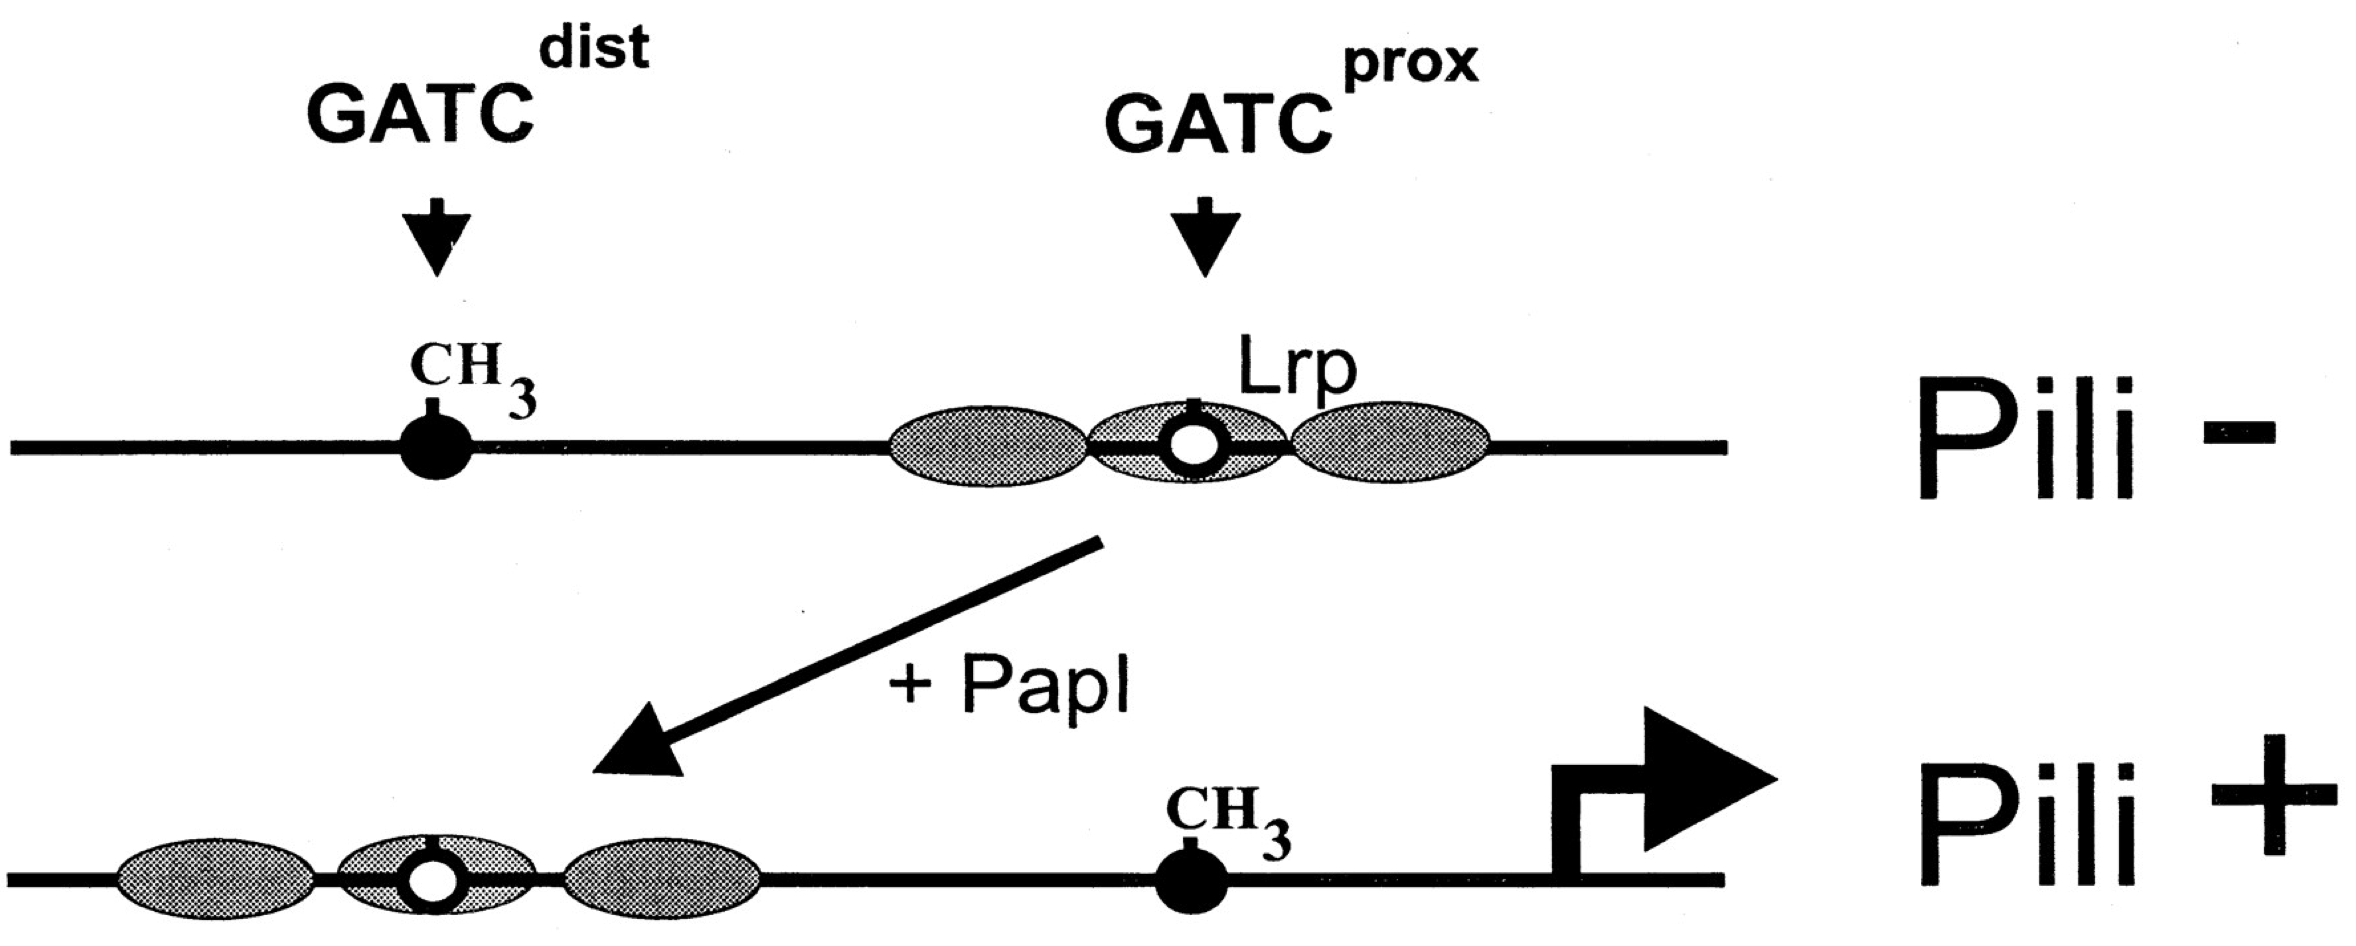
\includegraphics[scale=0.3]{text/Pictures/papPili.png}
	\caption{Scheme of the \tax{pap} phase OFF to ON switch. (reproduced from \cite{low2001roles})}
	\label{pap}
\end{figure}
During the OFF phase \tax{pap} pili are not produced because Lrp occupies GATC$^{prox}$ site which remains nonmethylated on both strands while GATC$^{dist}$ is fully methylated.
Lrp in this position prevents binding not only by Dam but by $\sigma^{70}$ RNA polymerase as well inhibiting expression of \tax{papBA} gene \cite{weyand2000regulation}.
For switch to ON phase an initial Lrp dissociation from sites 1-3 is necessary.
This likely happens during replication when an opportunity for Lrp to bind the hemimethylated GATC$^{dist}$ site instead of GATC$^{prox}$ raises.
The probability of this switch depends on the level of regulatory protein PapI in the cell as complex PapI/Lrp has lower affinity to site 2 but binds more likely to hemimethylated sites 4-6 than to fully methylated DNA \cite{hernday2003mechanism}.
Besides Lrp release from GATC$^{prox}$ site enables access of Dam to it so it can become methylated which further reduces Lrp affinity to 1-3 sites.
Even though RNA polymerase's access to \tax{papBA} promoter is not blocked any more the expression itself requires cAMP-CAP \cite{weyand2001essential}.
When PapB is beeing produced it acts as a \tax{papI} gene transcription activator leading to a feedback loop which stabilizes the cells in ON phase \cite{forsman1989autoregulation}.
However the described transition from OFF to ON phase occurs with 100-fold lower frequency than vice versa \cite{blyn1990regulation}.
The process of this opposite transition i.e. from ON to OFF phase involves transfer of Lrp from GATC$^{dist}$ to GATC$^{prox}$ during replication but the exact mechanism is not fully understood yet \cite{adhikari2016dna}.

Another well known orphan MT in \tax{E. coli} is \textbf{Dcm} which methylates second cytosine in 5'-CC(A/T)GG-3' motif to 5-methylcytosine (5mC) \cite{marinus1973isolation}.
Even though neither this one is necessary for \tax{E. coli} survival and some strains were found lacking \tax{dcm} gene, link between certain genes expression and presence of this MT was described.
Dcm seems to slow down expression of ribosomal genes \tax{rplC} and \tax{rpsJ} and inhibit transcription of \tax{sugE} gene connected with higher antimicrobial resistance \cite{militello2012conservation, militello2014cytosine}.
Both is happening predominantly during early stationary phase.
Next study shows increased expression of stress response sigma factor RpoS in \tax{dcm} mutant \cite{kahramanoglou2012genomics}.
Recently additional 63 genes were discovered to be affected if Dcm activity is inhibited \cite{militello20165}.
Most of these genes are up-regulater during early stationary phase if methylation by Dcm is silenced.

Lastly \textbf{YhdJ} is an orphan MT methylating 3' adenine of 5'-ATGCAT-3' sequence to 6mA when overexpressed.
Deleting \tax{yhdJ} gene produces neither loss of viability of \tax{E. coli} nor changes in its phenotype.
In addition, the expression of the gene is very low under usual laboratory conditions and nothing is known about transcription regulation of the gene \cite{broadbent2007yhdj}.

\subsection{Predictive cell behaviour}
An ability to predict an upcoming change in the environment is beneficial for any organism.
No matter whether the change means a presence of antibiotic or just shift in carbon source availability.
If a bacterium is able to predict such event it has a fitness advantage over those who don't expect this to happen in that community.

Circadian rhythms in photoautotrophic Cyanobacteria can be considered as one example of predictive behaviour in bacterial world.
It consists of alternation between photosynthetic activity during day and nitrogen fixation at night.
This periodicity persists in complete darkness or light for days.
It can also be reset by light or dark pulses in a way that two genetically identical populations act in the opposite way (oxygen production or nitrogen fixation) in constant dark or light conditions at the same time \cite{kondo1993circadian}.
Similar oscillatory rhythm was described in a bacterium other than Cyanobacterium as well.
\tax{Rhodobacter sphaeroides} was observed to keep changing gene expression in circadian (aerobic conditions) or ultradian (anaerobic conditions) rythms \cite{min2005rhythmic}.
Recent study investigating connection between day-and-night cycle and overall gene expression of microbial mat suggest that daily rhythmicity might not be uncommon outside Cyanobacteria \cite{hornlein2018daily}.
They state that 50\% of the rhythmic genes was derived from phylum \tax{Proteobacteria}.

Next predictive behaviour with no connection to day-and-night regime was observed in \tax{E. coli}.
Naturally it faces recurrent transitions between mammalian gastrointestinal tract (GIT) - higher temperature, lower oxygen - and outside environment - lower temperature, higher oxygen.
Consistent with predictive behaviour \tax{E. coli} strongly represses genes responsible for aerobic metabolism to temperature increase (without change in oxygen levels) in laboratory conditions \cite{tagkopoulos2008predictive}.
While if the temperature drops correlation in up-regulation of aerobic metabolism genes occurs.
They also evolved this strain in conditions where an increase in temperature was followed by oxygen saturation and temperature decrease by anaerobic conditions.
The two responses were successfully decoupled after 1000 generations suggesting that anticipatory regulation can be evolved for and against.

A year later, prediction of maltose environment to lactose exposure in \tax{E. coli} was described \cite{mitchell2009adaptive}.
Evolution under high lactose concentrations without maltose resulted in loss in prediction of maltose exposure and evolved lines exhibit a big fitness disadvantage compared to ancestor upon lactose-maltose transition.
The same authors investigated anticipation of oxidative stress by yeast which occurs in its natural habitat upon transition from fermentation to respiration.
\tax{Saccharomyces cerevisiae} uses heat-shock, ethanol and low pH as cues to prepare for its coming without actually experiencing it at the time \cite{mitchell2009adaptive}.


\section{Natural selection on responses and memory}
The current knowledge about gene expression in prokaryotes shows that transcription is a fairly regulated process.
But how this regulation evolved under selection in natural conditions is not fully understood.
Hypothesis about selection acting on transcriptional sensitivity, noise and possible memory exist.
%%% FIND REFERENCES FOR THAT!!!
Some supporting evidence and experiments exist, yet a lot remains to unravel still.

\subsection{Selection on sensitivity}
It was mentioned above that cells possess mechanisms to modulate time-dependent sensitivity of gene expression to a signal (e.g. FFLs).
Some of them are overrepresented in living organisms over others compared to randomized networks \cite{shen2002network, mangan2003structure}.
Bacteria are thus under natural selection towards accurate timing of their responses.
But is concentration-dependent sensitivity to a signal under selective pressure as well?
Common sense says there should be selection towards the concentration of a signal that is informative in the particular environment.
To the best of our knowledge no research investigated this so far.
%%% OR SHOULD I SAY "MY" KNOWLEDGE?
A possible way how to look into whether selection acts to reach certain level of sensitivity of promoters to a signal level is through experimental evolution.
Sensitivity of promoter variants from natural isolates could be then compared to those of lines evolved under low to high levels of an appropriate signal.
Looking simply at the distribution of concentration sensitivity of naturally occurring promoters could also provide useful information in this matter.

\subsection{Selection on noise}
Prior works have clearly shown that expression noise is evolvable \cite{richard2014does}.
Generally essential, constitutional genes and genes with high effect on overall expression (i.e. some transcription factors) tend to have low transcriptional noise \cite{silander2012genome, metzger2015selection}.
In constrast another interesting study describes higher noise in promoters from natural isolates of \tax{E. coli} compared to those of experimentally evolved lines just for their mean expression \cite{wolf2015expression}.
These results suggest that for different genes and/or at different niches there is a different optimum of transcriptional noise.
Indeed, a very recent study of the effect of expression noise on fitness of \tax{Saccharomyces cerevisiae} reveals that high noise is beneficial when expression level is far from optimum and vice versa \cite{duveau2018fitness}.
They also indicate that after introduction of an organism into a new environment selection might act towards high noise in expression of some genes before an appropriate expression plasticity evolves.
However, mutations in promoter regions usually change both expression level and noise at the same time \cite{metzger2015selection}.
Besides microorganisms some work in this area on other model organisms such as \tax{Drosophila melanogaster} \cite{schor2017promoter} and mouse \cite{barroso2017evolution} has been done as well.

\subsection{Selection on memory}
As mentioned above some bacteria are able to predict upcoming event based on othervise unrelated signal \cite{kondo1993circadian, min2005rhythmic, tagkopoulos2008predictive, mitchell2009adaptive}.
Microorganisms can also react faster to a signal if they were exposed to the same singal in past \cite{novick1957enzyme, mathis2017asymmetric}.
And in the case of epigenetic bistability, a subpopulation remains in a different physiological state than the rest of the culture in response to a signal \cite{arnoldini2014bistable, ronin2017long}.

An attempt of evolution of classical Pavlovian reflex to originally neutral signal in microorganisms was published last year \cite{lopez2017adaptive}.
As the neutral signal caffeine was added to media which yeast \tax{S. cerevisiae} was expected to associate with upcoming 5-fluoroorotic acid presence (metabolised into a toxic substance).
This predictive-like response appeared just within few hundred generations, but was not stable over time.
Thus, little is still known whether microorganisms are able to evolve such reflex to neutral cues in laboratory conditions.
The papers mentioned above suggest so \cite{tagkopoulos2008predictive, mitchell2009adaptive} and a mathematical model supports this hypothesis if benefits of such prediction exceed its costs in other environments \cite{mitchell2011mathematical}, but no experimental evidence is available so far.
Nevertheless the reported decoupling of reaction to a signal in the absence of expected outcome is a good indication of selection acting on predictive behaviour \cite{tagkopoulos2008predictive, mitchell2009adaptive}.




\section{Natural variation in responses and memory}
%%% swapped paragraph from 0.1 Taxonomy and characteristic of E. coli
Although the presence of \tax{E. coli} in water is still widely used as an indicator of fecal contamination recent studies show that some \tax{E. coli} isolates are able to  reproduce in soil \cite{byappanahalli2004indigenous, somorin2016general}.
Moreover strains inhabiting soil for a long time were found to be distinctive \cite{walk2009cryptic, walk2015cryptic}.
This raises the questions how these bacteria survive outside their hosts and how do they evolve under such conditions.


\cleardoublepage



\HeadingObjectives
\chapter*{Objectives}
\addcontentsline{toc}{chapter}{Objectives}

\shorthandoff{-} 

I will use a collection of environmental \tax{E. coli} strains isolated near Lake Superior, MN, USA \cite{ishii2006presence}.
These strains are distributed across the whole phylogenetic tree of the species.
They will be used in order to elucidate how natural selection acts on transcriptional responses and epigenetic memory of several promoters by investigating both genotypic and phenotypic variation among them.

\begin{enumerate}[font=\bfseries]

    \item \textbf{Quantify genotypic and phenotypic variation in promoters among environmental \tax{E. coli} isolates}
    
    In order to quantify variation in transcriptional responses, we will focus initially on studying natural variation in the response of the \tax{lac} operon in the presence of different carbon sources, both separately and in combination.
    To begin, we will study these responses using a plasmid-based system with transcriptional fusion.
    Previously, initial data comparing environmental strain SC1\textunderscore D9 and a lab strain MG1655 were collected which suggested that differences in the \tax{lacZ} promoter sequence and further downstream in \tax{lacZ} gene itself result in differential gene expression.
    Moreover, not only the sequence but also the genetic background of the strain was observed to affect the level of expression (i.e., both cis- and trans-effects are present).
    I will follow up on and expand these findings with \tax{lacZ} promoter and include four other promoters and ten environmental \tax{E. coli} strains as well.
    The specific steps of this objective are described further below.

    \begin{enumerate}[font=\bfseries]
    
        \item \textbf{Select promoter sequences among environmental \tax{E. coli} isolates to study}
        
        To begin we have selected the well-studied \tax{lacZ} and \tax{recA} promoters, because each creates a different type of cell response - carbon source catabolism and stress response, respectively.
        We will select three other transcriptional circuits to study as well.
        Promoters with known function and regulation mechanism will be picked based on an annotated MG1655 genome.
        Then we will search for corresponding sequences in genomes of natural isolates and identify the sequence differences in them.
        As we want to cover a broad variation scale on the genetic level, we will select promoter sequences which are both highly and slightly diverse among natural isolates.
        Those which are mainly bound by RNA polymerase with a conventional $\sigma^{70}$ factor will be preferred.

        \item \textbf{Quantify phenotypic variation in promoters using plasmid system}
        
        As we have a comprehensive collection of MG1655 promoters cloned on plasmids upstream of a fluorescent reporter (GFP gene) available \cite{zaslaver2006comprehensive}, next step after the promoter selection is to transform selected MG1655 promoters on these plasmid systems into chosen environmental \tax{E. coli} strains.
        Transcriptional responses of those will be analysed under sets of conditions (e.g., different carbon sources for \tax{lacZ} promoter, exposure to sublethal concentrations of an antibiotic for \tax{recA} promoter) using flow cytometry.
        This will be done to determine whether there are differential expression means, variance levels and dynamics of promoters originating from MG1655 among environmental strains (i.e., exploring trans-effects).
        Further, we will also clone promoters originating from chosen environmental strains upstream of the fluorescent reporter into the same plasmid system.
        These \tax{promoter::GFP} systems will be cloned into their source strains and MG1655 and tested under appropriate sets of conditions as well.
        A subset of studied strains will also be picked to compare patterns acquired from flow cytometry under dynamic conditions.
        Fluorescent microscopy and microfluidics will be used for this.
        Besides studying the transcriptional responses only, microfluidics will allow us to look into how the activity of selected promoters reacts in a fluctuating environment and thus investigate the occurrence of epigenetic memory in those transcriptional networks.
        
        \item \textbf{Confirm observed relationships between genotypic and phenotypic variation by chromosomal integration}
        
        Plasmid-based models are relatively fast and easy to acquire, but they might cause problems in interpreting the results.
         For example, there is usually a single copy of promoter present in bacterial chromosome, while there are often multiple copies of a plasmid in a cell.
        There might also be different transcriptional activities on a plasmid compared to a chromosome, e.g., depending on NAPs binding.
        To check whether this is the case in studied promoters, we will clone a subset of promoters showing differential expression upstream of a fluorescent reporter and then integrate them into the chromosome of studied strains.
        We will then monitor variation under the same sets of conditions as for plasmid-based models (e.g., different carbon sources or sublethal concentration of antibiotic).
        Flow cytometry will be used for this.
        If different expression patterns are observed when compared to plasmid models, we will continue studying the expression of such promoters after chromosomal integration only.
        Thus fluorescent microscopy and microfluidics will be performed on a subset of strains having a promoter with fluorescent reporter integrated into a chromosome and showing various expression dynamics among promoters under flow cytometry.

    \end{enumerate}
    
    \item \textbf{Compare natural variation in transcriptional responses with neutral model}
    
    Results from the previous aim will give us some view on how much natural variation there is in expression, sensitivity, plasticity, and noise and also whether epigenetics plays a role in any of the selected transcriptional networks.
    However, to understand whether natural selection has acted to increase or decrease variation in such transcriptional traits, we need a neutral model to compare to.
    Thus, we will generate sets of promoters with random mutations - i.e., variation expected to occur if there is no selection acting on neither of the traits of chosen promoters.
    Such an approach might also help us determine whether there is natural selection acting on memory.
    This will be achieved by random mutagenesis and analysis of variation produced this way as described below.

    \begin{enumerate}[font=\bfseries]
    
        \item \textbf{Generate libraries of promoters by random mutagenesis}
        
        First, we need to create random variation in the selected promoters.
        Error-prone polymerases will be used for that.
        We will aim for promoters with one to several SNPs within the promoter sequence.
        A library of the variants will be then cloned upstream of a fluorescent reporter into a plasmid or further incorporated into the chromosome of all studied genotypic backgrounds.
        Chromosomal integration will be chosen over a plasmid-based model if the previous results show differences in expression between these two approaches.

        \item \textbf{Quantify phenotypic variation in promoters created by random mutagenesis}
        
        Next, we will measure the expression mean, variance and dynamics of randomly generated promoters in our environmental strains using fluorescent reporter assays (plasmid system or chromosomal integration) and flow cytometry.
        The same sets of conditions that were used for native promoters will be applied here (i.e., different carbon sources for \tax{placZ}, exposure to a various sublethal concentration of antibiotics for \tax{precA}).
        The variance in these values will be then compared to variance obtained in native promoters among selected strains.
        Based on the results we will be able to define whether the selection has acted to decrease or increase certain traits (i.e., expression level, noise, sensitivity, plasticity).
        In the cases when memory is observed in naturally occurring promoter variants, we will also check whether it is still present when appropriate promoters after the random mutagenesis are used.
        For this, a subset of strains with adequate promoters from the neutral model will be picked and analysed under fluctuating conditions using microfluidics.
    
    \end{enumerate}

\end{enumerate}

\cleardoublepage%%% keeps correct headings

\shorthandon{-} 
%%%%%%%%%%%%%%%%%%%%%%%%%%%%%%%%%%%%


\HeadingChapters
\chapter{Materials and Methods}

\shorthandoff{-} 

\section{Strains and growth conditions}
All strains used in this work belong to the genus \tax{Escherichia coli} and are mainly derived from a classical laboratory strain K12 (MG1655) and an environmental strain SC1\textunderscore D9 isolated from a bank of St. Louis River in Minnesota \cite{ishii2006presence}.
In future work, additional environmental isolates will be used.

\begin{center}
    \begin{longtable}[c]{|l|c|c|c|c|}
\caption{Strains used in the study so far} \label{strains} \\

\toprule \multicolumn{1}{|l|}{\textbf{Strain ID}} & \multicolumn{1}{c|}{\textbf{Relevant genotype}} & \multicolumn{1}{c|}{\textbf{Promoter}} & \multicolumn{1}{c|}{\textbf{Ancestor}} & \multicolumn{1}{c|}{\textbf{Reference}} \\
\midrule
\endhead

\bottomrule
\endlastfoot

MG1655 & \tax{E. coli} K12 wild-type & - & - & \cite{blattner1997complete} \\
\hline
SC1\textunderscore D9 & \tax{E. coli} natural isolate & - & - & \cite{ishii2006presence} \\
\hline
pUA66-K12 & pUA66 & - & MG1655 & \cite{zaslaver2006comprehensive} \\
\hline
pU139-K12 & pU139 & - & MG1655 & \cite{zaslaver2006comprehensive} \\
\hline
pU139-D9 & pU139 & - & SC1\textunderscore D9 & this study \\
\hline
ASC662 & \tax{lacZ-GFP} & - & MG1655 & \cite{kiviet2014stochasticity} \\
\hline
pZ1\textunderscore K12-K12 & \tax{placZ::GFP} & MG1655 & MG1655 & \cite{zaslaver2006comprehensive} \\
\hline
pZ2\textunderscore K12-K12 & \tax{placZ::GFP} & MG1655 & MG1655 & this study \\
\hline
pZ2\textunderscore K12-D9 & \tax{placZ::GFP} & MG1655 & SC1\textunderscore D9 & this study \\
\hline
pZ\textunderscore D9-D9 & \tax{placZ::GFP} & SC1\textunderscore D9 & SC1\textunderscore D9 & this study \\
\hline
pZ\textunderscore D9-K12 & \tax{placZ::GFP} & SC1\textunderscore D9 & MG1655 & this study \\
\hline
pZm1\textunderscore D9-K12 & \tax{placZm172::GFP} & SC1\textunderscore D9 & MG1655 & this study \\
\hline
pZm2\textunderscore D9-K12 & \tax{placZm279::GFP} & SC1\textunderscore D9 & MG1655 & this study \\
\hline
pA\textunderscore K12-K12 & \tax{precA::GFP} & MG1655 & MG1655 & \cite{zaslaver2006comprehensive} \\
\hline
pA\textunderscore K12-D9 & \tax{precA::GFP} & MG1655 & SC1\textunderscore D9 & this study \\
\hline
Top10 & \text{*} & - & MG1655 & [Invitrogen] \\
\hline
pLW001-Top10 & pLW001 & - & Top10 & this study \\
    \end{longtable}
\footnotesize
    \emph{\text{*}} F– mcrA $\Delta$(mrr-hsdRMS-mcrBC) $\Phi$80lacZ$\Delta$M15 $\Delta$lacX74 recA1 araD139 $\Delta$(ara leu)7697 galU galK rpsL(Str$^{R}$) endA1 nupG\\*
\end{center}
\pagebreak

For flow cytometry and microscopy purposes, M9 minimal medium supplemented with 0.4\% of a single carbon source is used.
As those D(+)-glucose, lactose, D(+)-galactose, L-arabinose, and D(-)-ribose were chosen.
In other cases in LB medium (1.5\%~agar or liquid) is used.
Kanamycin to concentration 50 $\mu$g/ml is also added to the media if the bacterium contains pU139 or pUA66 plasmid (with or without promoter upstream of GFP).
All strains are grown at 37$^{\circ}$C, except for pLW001-Top10 which is grown at 30$^{\circ}$C (and in the presence of 100 $\mu$g/ml Ampicillin as well).


\hypertarget{MIC}{\section{Susceptibility test}}
To find out minimum inhibitory concentration to Ciprofloxacin cells are first grown in 96-well microplate in 18 replicates in M9 minimal medium supplemented with 0.4\% glucose.
Kanamycin to concentration 50 $\mu$g/ml is added to the media as well if the bacterium contains pU139 or pUA66 plasmid.
After 24 h incubation at 37$^{\circ}$C with shaking, the cells are transferred into the same fresh media by a pin replicator, but this time with an increasing concentration of Ciprofloxacin: 0, 5, 10, 15, 20 and 25 ng/ml.
This results in triplicates of each strain per particular Ciprofloxacin concentration.
Another 24 h incubation at 37$^{\circ}$C with shaking follows.
Next, the final optical density (OD) of the cultures at wavelength 600 nm is measured by a plate reader, and these values are then plotted using R (version 3.4.3).


\section{DNA isolation, PCR and sequencing}
For sequencing and cloning purposes 0.5 ml of LB supplemented with an appropriate antibiotic is inoculated by a single colony of desired strain and grown for 8 h at 37$^{\circ}$C or for 16 h at 30$^{\circ}$C with shaking.
5 $\mu$l of this culture is transferred into 100 $\mu$l of sterile deionized water and incubated at 95$^{\circ}$C for 5 min.
Isolated DNA is stored at -20$^{\circ}$C freezer.
For screening of positive clones, a colony PCR is performed.

\begin{center}
    \begin{longtable}[c]{|l|c|c|c|}
\caption{List of primers} \label{pcr} \\

\toprule \multicolumn{1}{|l|}{\textbf{Primer}} & \multicolumn{1}{c|}{\textbf{Sequence 5' -- 3'}} & \multicolumn{1}{c|}{\textbf{T$_{a}$}} & \multicolumn{1}{c|}{\textbf{Purpose}} \\
\midrule
\endhead

\bottomrule
\endlastfoot

pUA66\textunderscore insert\textunderscore R & \footnotesize{\texttt{TCGCAAAGCATTGAAGACCATACGC}} & \multirow{2}{*}{56$^{\circ}$C} & \multirow{2}{*}{sequencing} \\
pUA66\textunderscore insert\textunderscore F & \footnotesize{\texttt{TTGTCTGTTGTGCCCAGTCATAGC}} & & \\
\hline
pUA66\textunderscore clon\textunderscore R & \footnotesize{\texttt{CGCATAGGGCCCGGATTTGTCCTACTCAGGAGAGCG}} & \multirow{2}{*}{54$^{\circ}$C} & \multirow{2}{*}{cloning} \\
pUA66\textunderscore clon\textunderscore F & \footnotesize{\texttt{TAAGGTCCCGGGCTGTCTCTTGATCAGATCTTGATCCCC}} & & \\
\hline
ATT-RP2 & \footnotesize{\texttt{CAGAATCCCTGCTTCGTCCA}} & \multirow{2}{*}{55$^{\circ}$C} & \multirow{2}{*}{sequencing} \\
PSC-FP2 & \footnotesize{\texttt{TATCGAATCAAAGCTGCCGA}} & & \\
    \end{longtable}
\end{center}

In case of screening DreamTaq Green PCR Master Mix (2X) is used for PCR according to manufacturer's \href{https://assets.thermofisher.com/TFS-Assets/LSG/manuals/MAN0012704_DreamTaq_Green_PCR_MasterMix_K1081_UG.pdf}{instructions}.
The PCR is run at these conditions: 3~min @ 95$^{\circ}$C; 35 cycles: 30~s @ 94$^{\circ}$C + 30~s @ T$_{a}$ + 60~s/kb @ 72$^{\circ}$C; 5~min @ 72$^{\circ}$C.
For sequencing PCR with recombinant \tax{Taq} DNA polymerase [Invitrogen] is performed according to manufacturer's \href{https://assets.thermofisher.com/TFS-Assets/LSG/manuals/0814_Taq_DNA_Polymerase_recombinant.pdf}{instructions}.
PCR conditions are as follows: 3~min @ 95$^{\circ}$C; 35 cycles: 45~s @ 94$^{\circ}$C + 30~s @ T$_{a}$ + 90~s/kb @ 72$^{\circ}$C; 10~min @ 72$^{\circ}$C. Used T$_{a}$ for different primers are listed in Table~\ref{pcr}.

PCR products are column purified before dispatch for Sanger sequencing to Macrogen, Korea.
Column purification is performed using E.Z.N.A.\textsuperscript{\textregistered} Cycle Pure Kit according to manufacturer's \href{http://omegabiotek.com/store/wp-content/uploads/2013/09/D6492_D6493-Cycle-Pure-Kit-Combo-Online.pdf}{centrifugation protocol}.
Purified DNA is eluted into 30 $\mu$l of sterile deionized water.

\section{Cloning}
\subsection{TOPO TA cloning}
The desired insert is amplified from donor strain using pCR\textsuperscript{TM}8/GW/TOPO\textsuperscript{\textregistered} reagents according to manufacturer's \href{https://assets.thermofisher.com/TFS-Assets/LSG/manuals/pcr8gwtopo_man.pdf}{instructions}, except for recombinant \tax{Taq} DNA polymerase [Invitrogen] and primers (see Table \ref{pcr}).
PCR is run as follows: 3~min @ 95$^{\circ}$C; 35~cycles: 45~s @ 95$^{\circ}$C + 30~s @ T$_{a}$ + 90~s/kb @ 72$^{\circ}$C; 30~min @ 72$^{\circ}$C.
20 $\mu$l of PCR product is then column purified using E.Z.N.A.\textsuperscript{\textregistered} Cycle Pure Kit according to manufacturer's \href{http://omegabiotek.com/store/wp-content/uploads/2013/09/D6492_D6493-Cycle-Pure-Kit-Combo-Online.pdf}{centrifugation protocol}.
Purified DNA is eluted into 30 $\mu$l of sterile deionized water.

TOPO\textsuperscript{\textregistered} Cloning reaction is performed according to manufacturer's \href{https://assets.thermofisher.com/TFS-Assets/LSG/manuals/pcr8gwtopo_man.pdf}{instructions} with 4 $\mu$l of purified PCR product.
The reaction is incubated at 22$^{\circ}$C for 30~min and stored in -20$^{\circ}$C freezer before electroporation or One Shot\textsuperscript{\textregistered} Chemical transformation.
In the case of using chemical transformation, it is performed according to manufacturer's \href{https://assets.thermofisher.com/TFS-Assets/LSG/manuals/pcr8gwtopo_man.pdf}{instructions} and using their S.O.C. medium.

\subsection{Construction of pADOUCH plasmid}
First pLW001 vector and TOPO vector with the desired insert (see TOPO TA cloning above) are isolated from donor strains grown in liquid LB supplemented with an appropriate antibiotic.
This is performed using StrataPrep Plasmid Miniprep Kit according to manufacturer's \href{https://www.agilent.com/cs/library/usermanuals/public/400766.pdf}{instructions}.
Changes are made in using sterile deionized water instead of elution buffer and growing pLW001-Top10 donor strain for 24 h at 30$^{\circ}$C before the very plasmid isolation.
Restriction digestion is then set up using ApaI and XmaI restriction enzymes in the final volume of 50 $\mu$l with incubation at 25$^{\circ}$C for 2 h followed by 37$^{\circ}$C for another 2~h.
Digested pLW001 vector is then dephosphorylated with rSAP treatment at 37$^{\circ}$C for 30~min, and both reactions are subsequently heat inactivated at 65$^{\circ}$C for 30 min.

Digested vector and insert are gel extracted using StrataPrep DNA Gel Extraction Kit according to manufacturer's \href{https://www.agilent.com/cs/library/usermanuals/public/400766.pdf}{instructions} with the exception that 50 $\mu$l of sterile deionized water is used for elution instead of elution buffer.
Overnight ligation at 16$^{\circ}$C is then performed using T4 ligase in the final volume of 20 $\mu$l and keeping DNA concentration between 1-10 ng/$\mu$l.
The ligation reaction is used directly for electroporation or stored in -20$^{\circ}$C freezer before use.

\section{Transformation}
Desired plasmids for transformation are isolated from donor strains grown in liquid LB supplemented with an appropriate antibiotic and using StrataPrep Plasmid Miniprep Kit according to manufacturer's \href{https://www.agilent.com/cs/library/usermanuals/public/400766.pdf}{instructions}.
The only exceptions are using sterile deionized water instead of elution buffer and growing pLW001-Top10 strain for 24 h at 30$^{\circ}$C before the very plasmid isolation.
If the concentration of acquired plasmid DNA is too low, it is concentrated using centrifugal vacuum concentrator [Eppendorf\textsuperscript{\textregistered} Basic Model 5301] at room temperature.
In the case of transformation by ligation mixture, this is used directly without any purification.

\subsection{TSS transformation}
A flask of 100~ml capacity containing 10~ml of liquid LB is inoculated by 0.1~ml of overnight MG1655 culture (for other strains or plasmid size above 5~kb electroporation is used) and incubated at 37$^{\circ}$C with shaking.
When OD$_{600}$ rises to values between 0.5 -- 0.9 the culture is fast chilled by swirling in ice slurry for 15~min.
Next 0.75~ml of the chilled culture is transferred into a 5~ml tube containing the same amount of ice cold 2x TSS (see Table \ref{tss}) and is incubated on ice slurry for 30~min.
2~$\mu$l of the desired plasmid is then added to the cells with subsequent incubation on ice slurry for another 1~h.
After an additional incubation for 1~h at 37$^{\circ}$C with shaking, cells are centrifuged at maximum speed (i.e., 20817~G) for 5~min at room temperature, the supernatant is discarded and the pellet re-suspended in 0.2~ml of LB.
From this 10-fold dilutions are prepared up to 10$^{-3}$, and these are spread by sterile beads on LB agar plates containing an appropriate antibiotic.
Non-diluted culture is plated as well.
Plates are then incubated overnight at 37$^{\circ}$C, and single colonies are checked for desired plasmid presence by PCR.

%\newpage

\begin{center}
    \begin{longtable}[c]{|l|c|c|}
\caption{Content of 2x TSS} \label{tss} \\

\toprule \multicolumn{1}{|l|}{\textbf{Component}} & \multicolumn{1}{c|}{\textbf{Amount per 100~ml of 2x TSS}} \\
\midrule
\endhead

\bottomrule
\endlastfoot

Bacto-Tryptone & 0.8~g \\
\hline
Yeast extract & 0.5~g \\
\hline
NaCl & 0.5~g \\
\hline
PEG 8000 & 20.0~g \\
\hline
1M MgSO$_{4}$ & 10~ml \\
\hline
DMSO & 10~ml \\
    \end{longtable}
\end{center}

\subsection{Preparation of electrocompetent cells}
A flask of 1 l capacity containing 100 ml of liquid LB is inoculated by 1 ml of overnight culture and incubated at 37$^{\circ}$C with shaking.
After reaching OD$_{600}$ between 0.5 -- 0.9 the culture is fast chilled by swirling in ice slurry for 5 -- 10 min and then kept in the slurry for 1 h.
Next, the culture is transferred into 2 pre-chilled 50 ml falcon tubes and centrifuged at 4$^{\circ}$C for 10 min at 4200 G.
The supernatant is discarded, and the pellet is washed twice in about 25 ml of 10\% glycerol with centrifugation at 4$^{\circ}$C for 10 min at 4500~G.
The final supernatant (about 0.5 ml) is pooled into one falcon tube and aliquoted into pre-chilled (in -80$^{\circ}$C freezer) 1.7 ml tubes.

\subsection{Electroporation}
A tube of electrocompetent cells is thawed on ice, and 1 $\mu$l of desired plasmid or 3 $\mu$l of ligation mix is added to it.
The cells are then transferred into 0.1 cm electroporation cuvette [BioRad] and electroporated at 1850 V (or 1800 V if vector is bigger than 10 kb) [Eppendorf Eporator\textsuperscript{\textregistered}].
500 ml of S.O.C. medium is added immediately to the cuvette, and the whole content then transferred into pre-warmed 5 ml tube.
After incubation for 1~h at 37$^{\circ}$C (or 2 h at 30$^{\circ}$C in case of pLW001 plasmid background) with shaking, 10-fold dilutions up to 10$^{-3}$ are prepared and spread by sterile beads on LB agar plates containing an appropriate antibiotic.
Non-diluted culture is plated as well.
Plates are then incubated overnight at 37$^{\circ}$C (or two overnights at 30$^{\circ}$C), and single colonies are checked for desired plasmid presence by a colony PCR.


\hypertarget{FC}{\section{Activity assays of promoters}}
\subsection{Promoter \tax{lacZ}}
M9 media with 0.4\% of chosen single carbon sources (0.2~ml) in 96-well microplates are inoculated by strains from a glycerol stock in triplicates using a pin replicator.
After overnight incubation at 37$^{\circ}$C without shaking the strains are transferred into the same fresh media by a pin replicator and incubated again at 37$^{\circ}$C without shaking for 4~h.
Before acquiring the data from samples with flow cytometer [BD FACSDiva version 6.1.3], all strains are 10-fold (MG1655 background) or 20-fold (SC1\textunderscore D9 background) diluted in 1x~PBS with $\sim$1\% formaldehyde.
Data from 10 -- 100 thousand events are collected using GFP filter 513/17 [BD] and exported into Flow Cytometry Standard (FCS) files.
These files are then analysed in R (version 3.4.3) using flowCore package (version 1.44.1) \cite{hahne2009flowcore}.
Scripts used for data analysis are available at \href{https://github.com/marketavlkova/LacZ_FC}{GitHub}.

\subsection{Promoter \tax{recA}}
M9 media supplemented with 0.4\% glucose, and Ciprofloxacin at sub-MIC concentrations (0.5~ng/ml, 1.0~ng/ml, 2.0~ng/ml and 4.0~ng/ml) in 96-well microplates are inoculated by strains from a glycerol stock in duplicates using a pin replicator.
Further steps are the same as for \tax{lacZ} promoter assay (using M9 with glucose and Ciprofloxacin).
Scripts used for data analysis of \tax{recA} promoter are available at \href{https://github.com/marketavlkova/RecA}{GitHub} in a separated repository.


\section{Microscopy}
For fluorescent microscopy, 1~$\mu$l of fresh 4~h culture (see promoter activity assay for growth conditions) is transferred to 1\% agarose pad prepared from the same media the cells are grown in.
Multiple agarose pads are placed within a single gene frame on a microscope slide and after adding cultures covered with a coverslip.
Two positions per an agarose pad are chosen and automated time-lapse phase contrast and fluorescent (GFP; 200~ms exposure time) microscopy is set-up.
Both phase contrast and fluorescent images are taken using 100x immersion objective and Hamamatsu camera [ORCA-Flash4.0].

All pictures are stored and further handled in TIFF format using Fiji ImageJ software.
To produce movies the fluorescent pictures are merged with the phase contrast ones (only focused pictures are used for this).
Next, the minimum and maximum pixel values of both channels are adjusted: fluorescent channel 0-4095 (i.e., 12-bit), phase contrast channel 0-65535 (i.e., 16-bit).
This is finally saved into AVI format.

\cleardoublepage%%% keeps correct headings

\shorthandon{-}
%%%%%%%%%%%%%%%%%%%%%%%%%%%%%%%%%%%%


\chapter{Results}

\shorthandoff{-} 

\section{Cloned \tax{promoter::GFP} sequences}
As most of the strains listed in the Table \ref{strains} were prepared several years ago and not by myself, we wanted to check which parts of the promoters we actually have cloned upstream of GFP gene in those cells.
For this purpose I designed pUA66\textunderscore insert primers (Table \ref{pcr}) based on the pUA66 and pU139 vector sequences (\hyperlink{pUA66seq}{Appendix 1} and \hyperlink{pUA66seq}{Appendix 2}).
PCR products were sequenced by Macrogen, Korea using Sanger platform.

\hypertarget{SeqRes}{\subsection{\tax{placZ::GFP} strains}}
In the Fig. \ref{placZ} we can see that SC1\textunderscore D9 and MG1655 differ in \tax{lacZ} promoter region by a single SNP at position 39 nt upstream from \tax{lacZ} gene start codon (position 199 in Fig. \ref{placZ}).
These 2 strains have 3 more SNPs further downstream in \tax{lacZ} gene itself 
(positions 306, 324 and 363 in Fig. \ref{placZ}).
Based on the alignment of acquired \tax{lacZ} promoters sequences (Fig. \ref{placZ}) we can confirm that those assumed to originate from SC1\textunderscore D9 have an appropriate sequence as well as for MG1655.
\begin{figure}[ht]
  \centering
  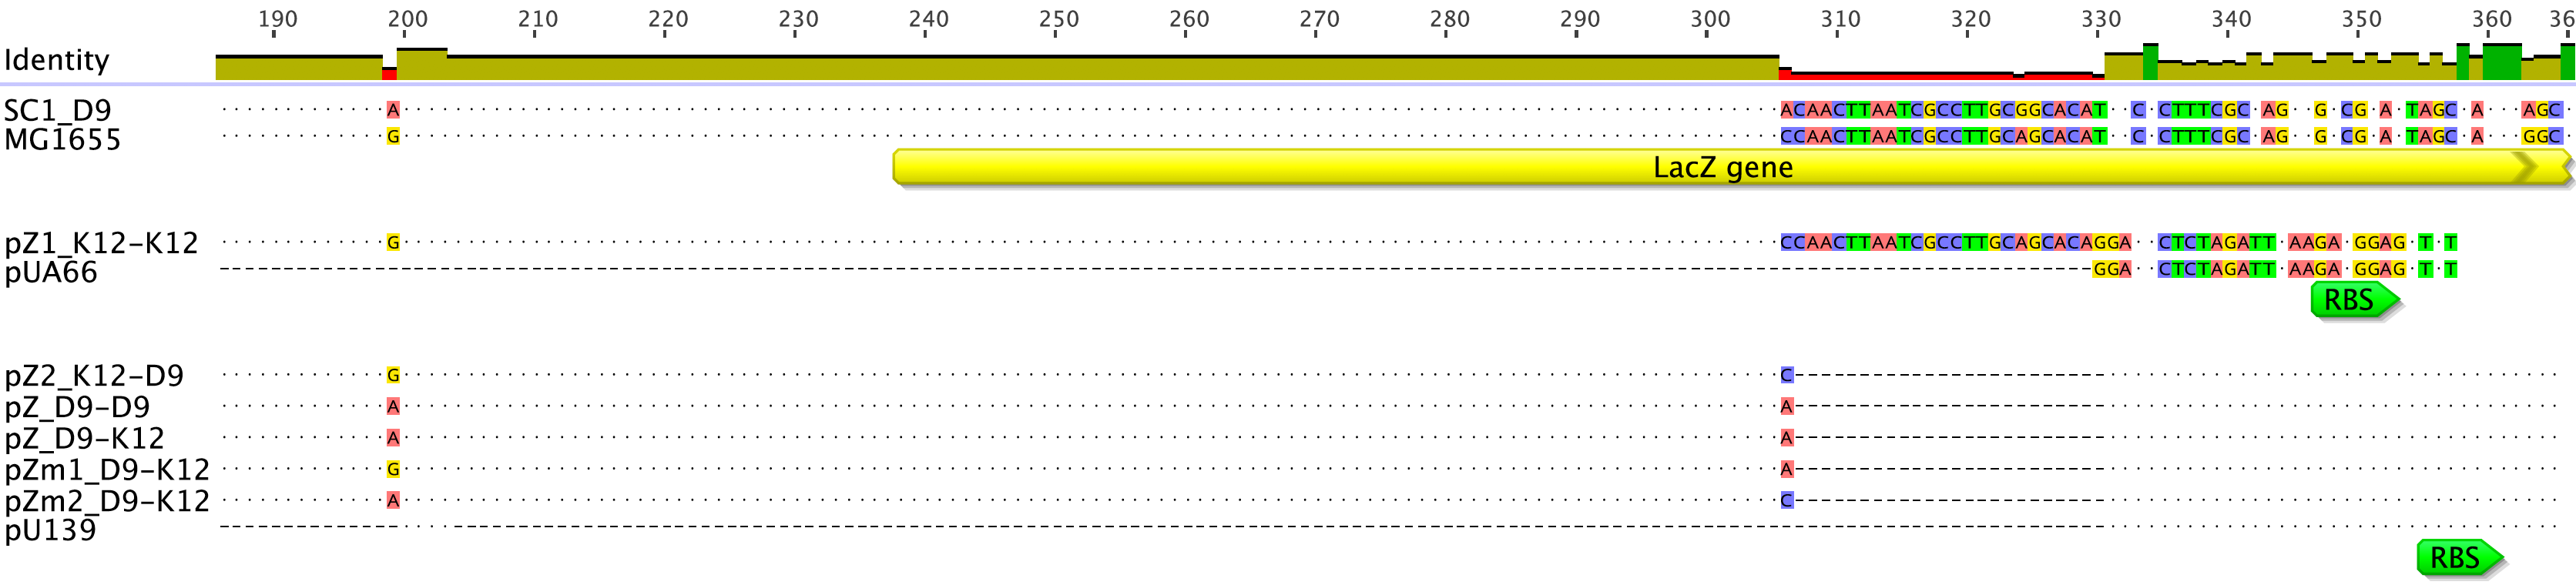
\includegraphics[scale=0.25]{text/Pictures/placZsequences.png}
	\caption{Excerpt of \tax{lacZ} promoters alignment with vectors and references. SC1\textunderscore D9 and MG1655 are reference sequences of \tax{lacZ} promoters from particular strains. pUA66 and pU139 are vectors aligned with no promoter upstream of GFP gene (not shown).}
	\label{placZ}
\end{figure}
Beside the SNPs in \tax{lacZ} promoter, the first SNP from \tax{lacZ} coding sequence is included in all vectors upstream of GFP.
Most of the strains possess pU139 as the vector except for pZ1\textunderscore K12-K12 which was acquired from Alon library \cite{zaslaver2006comprehensive}.
This strain have also longer part of \tax{lacZ} gene cloned into its pUA66 vector, potentially covering second SNP in it when compared to SC1\textunderscore D9.
This is not the only difference of pZ1\textunderscore K12-K12, as part of the \tax{lacI} gene is incorporated in all sequences listed in Fig. \ref{placZ} on the opposite site of the promoter (\hyperlink{placZalign}{Appendix 3}) and pZ1\textunderscore K12-K12 has this \tax{lacI} sequence almost 60 bp shorter than the rest of these strains.
Note, that strain pZ1m1\textunderscore D9-K12 and pZ1m2\textunderscore D9-K12 possess a recurrent mutation of the SNP in \tax{lacZ} promoter or \tax{lacZ} gene, respectively (from SC1\textunderscore D9 back to MG1655).
You can also realize that strain pZ2\textunderscore K12-K12 is not included in the Fig. \ref{placZ}.
The reason is that it was made by transforming the plasmid from pZ2\textunderscore K12-D9 into MG1655 after receiving the sequencing data and was not sequenced afterwards.

\subsection{\tax{precA::GFP} strains}
Both pA\textunderscore K12-K12 and pA\textunderscore K12-D9 strains have the same plasmid (pU139) as the latter was made by transforming plasmid from the former.
It was also confirmed by sequencing as well as that the sequence upstream of GFP gene correspond to \tax{recA} promoter of MG1655 (\hyperlink{precAalign}{Appendix 4}).
Similar to the cloned \tax{lacI}-\tax{lacZ} intergenic regions mentioned above, the sequence incorporated into pU139 and then transformed into these \tax{precA::GFP} strains includes parts of \tax{recA} gene downstream and \tax{pncC} gene upstream of the very promoter.


\section{Ciprofloxacin susceptibility}
Because we want to induce \tax{recA} promoter by exposing the cells to a sub-lethal (i.e. sub-MIC) exposure to Ciprofloxacin, I had to make sure the strains I use are susceptible to Ciprofloxacin, first.
I wanted also to estimate what are the minimum inhibitory concentrations (MICs) for this antibiotic in the strains used.
MG1655 and SC1\textunderscore D9 were incubated in an increasing concentration of Ciprofloxacin (see \hyperlink{MIC}{Materials and Methods}).
\begin{figure}[b!]
  \centering
  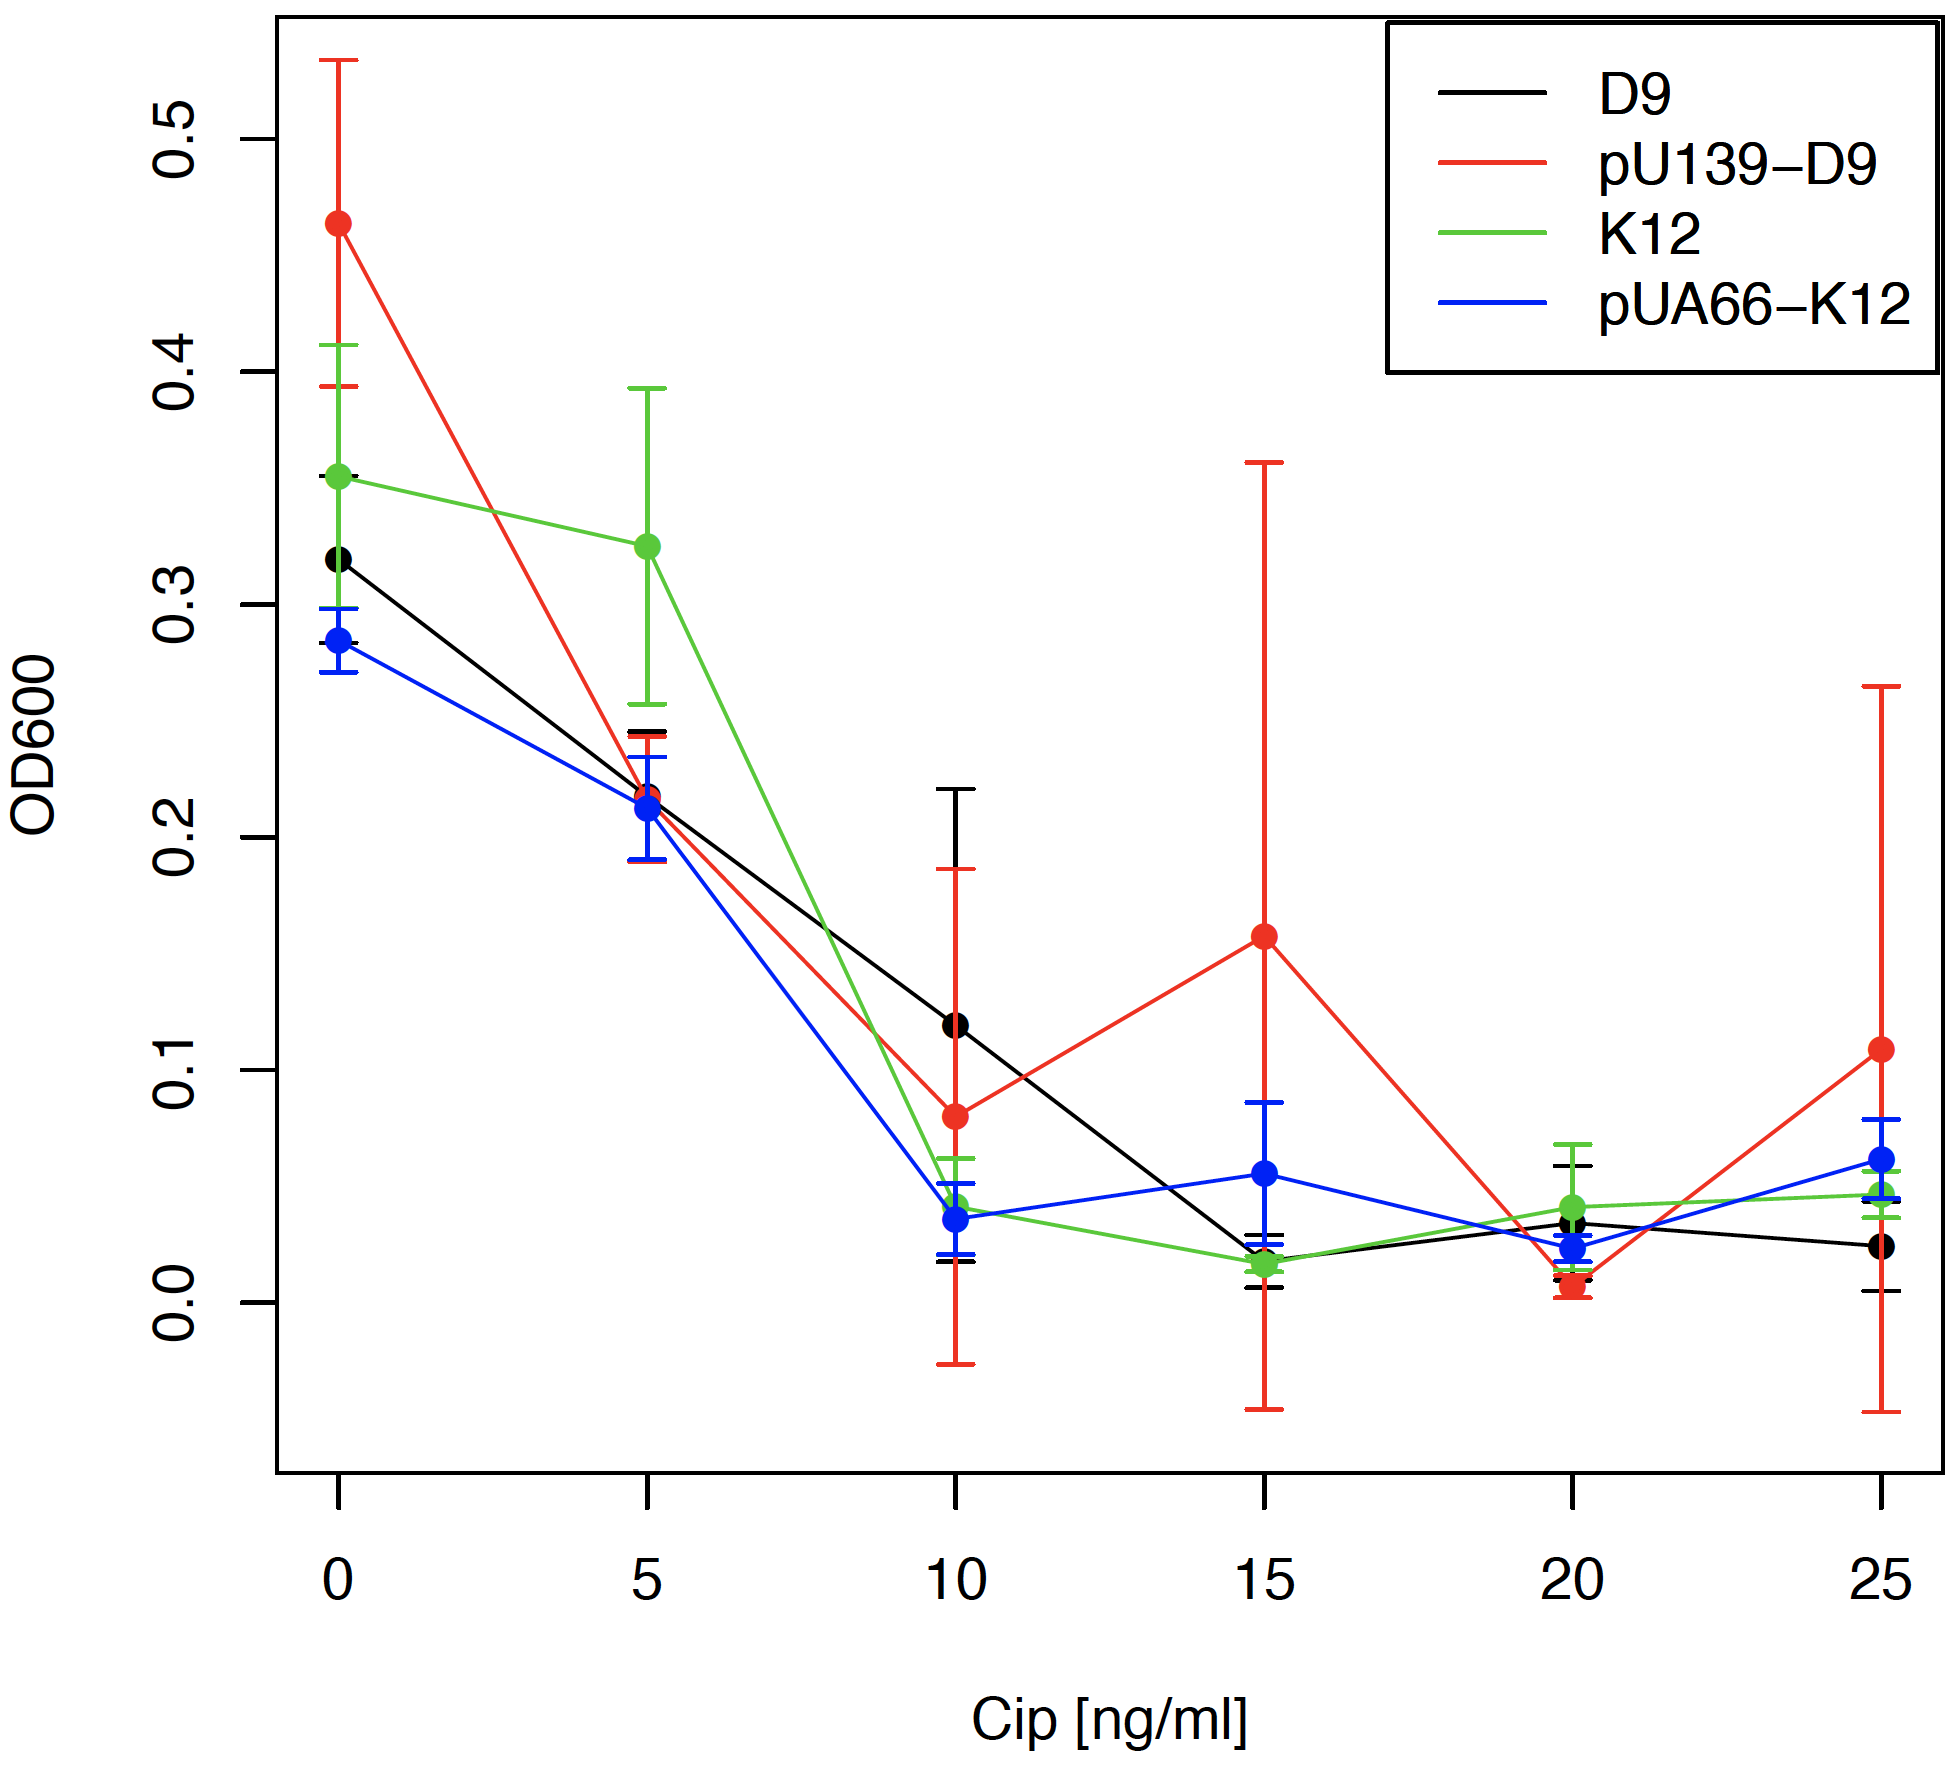
\includegraphics[scale=0.25]{text/Pictures/KillCurve.png}
	\caption{Cell density after 24 h growth of MG1655 and SC1\textunderscore D9 strains in various Ciprofloxacin concentrations. Strains with a promoter-less plasmid are also included.}
	\label{killing}
\end{figure}
Strains with promoter-less pU139 or pUA66 plasmid were also included to ensure the Kanamycin resistance carried on the plasmid does not affect Ciprofloxacin sensitivity.
The MIC for both strains is 10 ng/ml of Ciprofloxacin or less, however 5 ng/ml is the concentration which both strains are able to survive, although a decrease in the final cell density is observed when compared to the growth in the absence of Ciprofloxacin (Fig. \ref{killing}).
Plasmid carried Kanamycin resistance causes none or small effect on Ciprofloxacin susceptibility.


\section{Variation in promoter activity}
To explore the differences in promoter activity and genetic backgrounds, 4 h cultures grown in M9 minimal media with a single carbon source were assayed using flow cytometry (see \hyperlink{FC}{Materials and Methods}).
Exported FCS files were then analysed in R - used scripts are available at \href{https://github.com/marketavlkova/}{GitHub} repositories.

\subsection{Activity of \tax{lacZ} promoters}
\subsubsection{Expression in lactose environment}
All strains with \tax{lacZ} promoter cloned upstream of GFP gene and strain ASC662, which has GFP integrated into chromosome in \tax{lac} operon, show strong GFP expression when grown in lactose as a sole carbon source (Fig. \ref{lacZassay}).
All plasmid based models show about 2.5 to 10.5 times (3.842 au $\pm$ 0.113 in pZ1\textunderscore K12-K12 to 4.464 au $\pm$ 0.095 in pZm1\textunderscore D9-K12) higher GFP expression than ASC662 (3.442 au $\pm$ 0.140).
Differences are observed, as expected, when a promoter sequences of the same length originating from different strains are cloned into the same genotypic background.
Strain pZ\textunderscore D9-D9 has over 1.5 times higher mean GFP expression than pZ2\textunderscore K12-D9 (4.403 au $\pm$ 0.202 and 4.219 au $\pm$ 0.134, respectively).
Similarly, pZ\textunderscore D9-K12 has almost 1.5 times higher mean expression than pZ2\textunderscore K12-K12 (4.437 au $\pm$ 0.117 and 4.267 au $\pm$ 0.103, respectively).
Over 2.5-fold difference in expression is also observed when comparing both strains with two versions of cloned promoter sequence both originating from MG1655 into the same strain, i.e. pZ1\textunderscore K12-K12 and pZ2\textunderscore K12-K12.
The former having mean expression 3.842 au $\pm$ 0.113, the latter 4.267 au $\pm$ 0.103.

\begin{figure}[ht!]
  \centering
  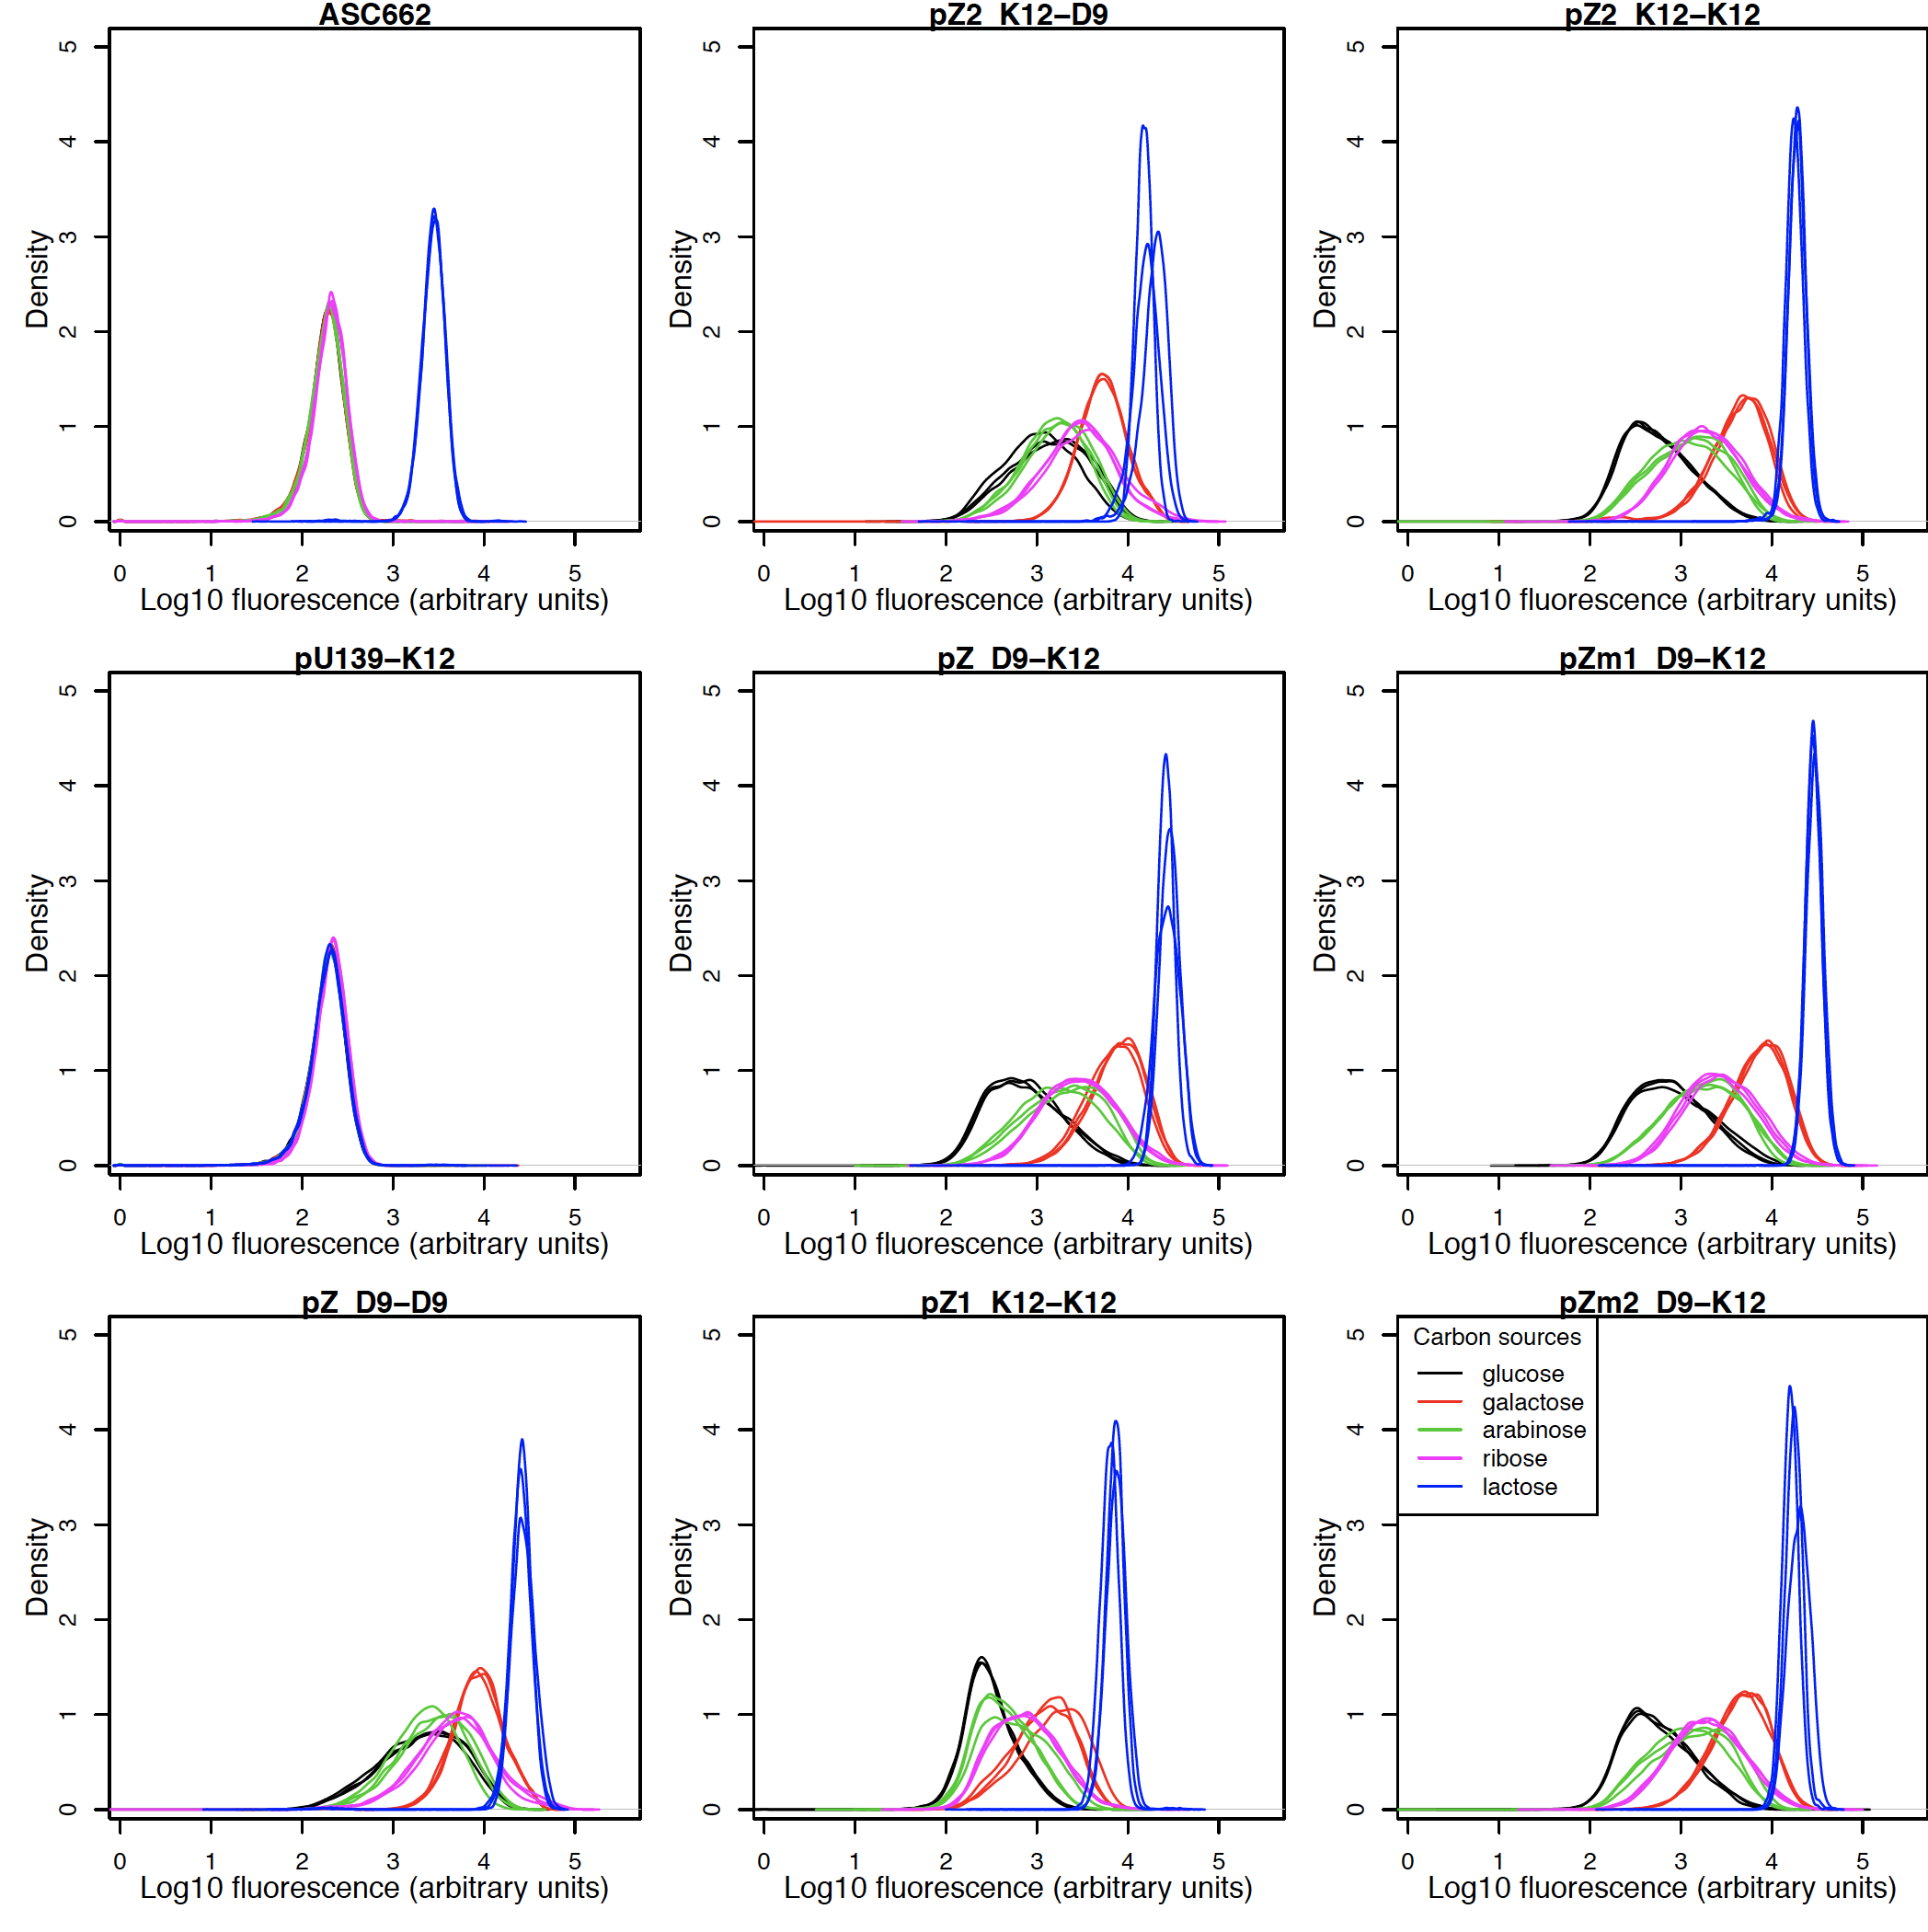
\includegraphics[scale=0.4]{text/Pictures/lacZassay.png}
	\caption{\tax{lacZ} promoter activity in various carbon sources. Strain ASC662 has GFP gene integrated into chromosome in \tax{lac} operon native locus. pU139-K12 is negative control of GFP expression for plasmid based models - promoter-less pU139 plasmid present. The rest are strains with various \tax{lacZ} promoters cloned upstream of GFP gene in a plasmid - see Table \ref{strains}.}
	\label{lacZassay}
\end{figure}

The strains pZ\textunderscore D9-K12 and pZ2\textunderscore K12-K12 differ just by the two SNPs in the sequence cloned upstream of GFP gene, while one of the SNPs is located in the cloned part of \tax{lacZ} gene, not in the promoter itself (see \hyperlink{SeqRes}{sequencing results}).
If the SNPs from \tax{lacZ} gene had no effect on the GFP expression we should see the same expression pattern in pZm1\textunderscore D9-K12 as in pZ2\textunderscore K12-K12 (i.e. 4.267 au $\pm$ 0.103).
However, this is not the case - the recurrent mutation of the first SNP (A to G) leads to even higher mean expression difference (4.464 au $\pm$ 0.095) than is seen with the original sequence from SC1\textunderscore D9 (4.437 au $\pm$ 0.117).
Interestingly we get much closer mean expression values to MG1655 promoter sequence with the recurrent mutation in the \tax{lacZ} coding sequence.
This time pZm2\textunderscore D9-K12 shows a bit lower expression level than pZ2\textunderscore K12-K12 (4.249 au $\pm$ 0.105 vs 4.267 au $\pm$ 0.103).

\subsubsection{Expression in non-lactose environments}
ASC662 does not express GFP when grown in any other carbon source used as the fluorescence levels are the same as for negative control pU139-K12.
Negative control for SC1\textunderscore D9 background i.e. pU139-D9 is comparable to pU139-K12 (\hyperlink{FCnegs}{Appendix 5}).
Interestingly some \tax{lacZ} promoter activity is observed in all plasmid model strains grown in any other carbon source, even glucose (Fig. \ref{lacZassay}).
Generally in all of them we can see the same pattern - an increasing \tax{lacZ} promoter activity based on the carbon source used: glucose $<$ arabinose $<$ ribose $<$ galactose $<$ lactose.
The difference in expression between arabinose and ribose environment is relatively small, but consistent among all strains and replicates.
Moreover the mean expression levels in all these carbon sources depends not only on the promoter variant the strain has, but also at the genetic background of the strain (see pZ\textunderscore D9-D9 vs pZ\textunderscore D9-K12 and pZ2\textunderscore K12-D9 vs pZ2\textunderscore K12-K12 in Fig. \ref{lacZassay}).
Note, that some density curves (mainly those from glucose growth) do not have the regular shape which is common for all samples from lactose growth.

\subsection{Activity of \tax{recA} promoter}

% 17.9.2018
% where is this name from?
\section{Construction of pADOUCH plasmid}
As we could see, \tax{lacZ} promoters cloned into plasmids were active even in non-lactose environments, but that is not the case if GFP gene is integrated into chromosome.
We hypothesise, that this differential results might be caused by the naturally low amounts of LacI repressor present in a cell.
When a cell makes multiple copies of \tax{lacZ} promoter by its sequence on a plasmid, all LacI proteins become saturated and a part of the promoters escape the repression, even though the plasmids used should produce only several copies within a cell \cite{zaslaver2006comprehensive}.
To confirm that we decided to place the \tax{placZ::GFP} sequences into chromosome, creating only one additional \tax{lacZ} promoter per a cell.

We have available pLW001 plasmid which is suitable for chromosomal integration (\hyperlink{pLW001}{Appendix 6}) however, this plasmid lacks ribosome binding site (RBS).
Thus we constructed a new plasmid by replacing the GFP gene present in pLW001 vector with the GFP sequence we have in our negative control plasmid pUA66 (\hyperlink{pUA66seq}{Appendix 1}) together with its strong RBS, some additional restriction sites and a transcriptional terminator (Fig. \ref{cloning}).
\begin{figure}[h!]
  \centering
  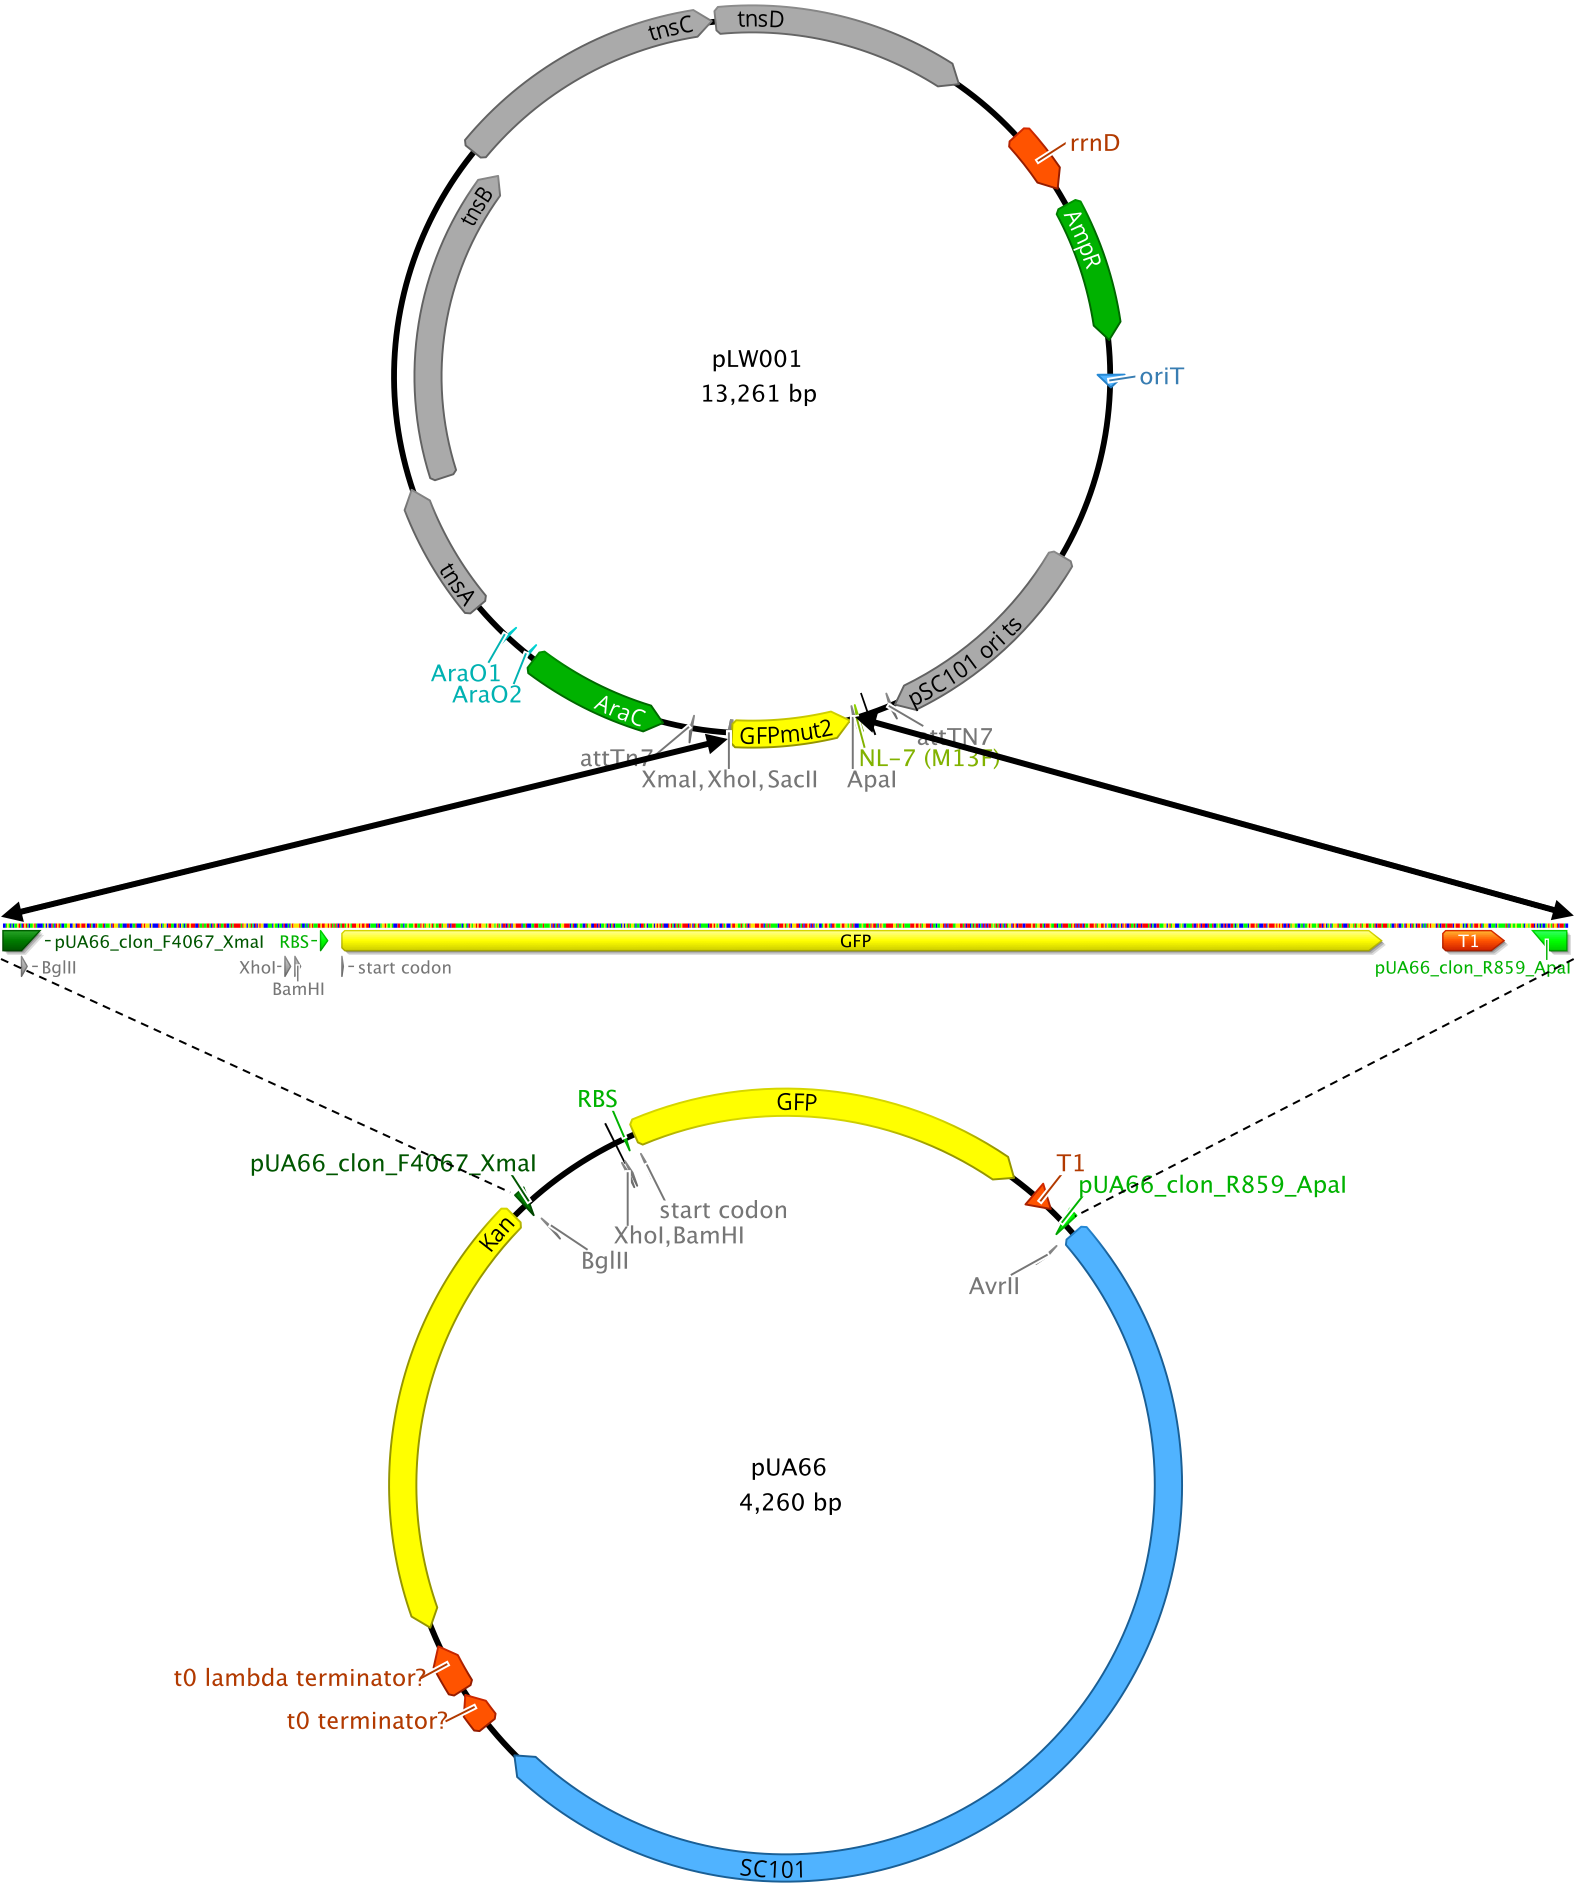
\includegraphics[scale=0.4]{text/Pictures/Cloning.png}
	\caption{Scheme of pADOUCH plasmid construction by replacing GFP sequence from pLW001 vector by sequence from pUA66 plasmid.}
	\label{cloning}
\end{figure}

We successfully amplified sequence of expected length (1.1 kb) in all 8 transformants tested (Fig. \ref{colonyPCR}), showing that successful integration had occurred.
\begin{figure}[h!]
  \centering
  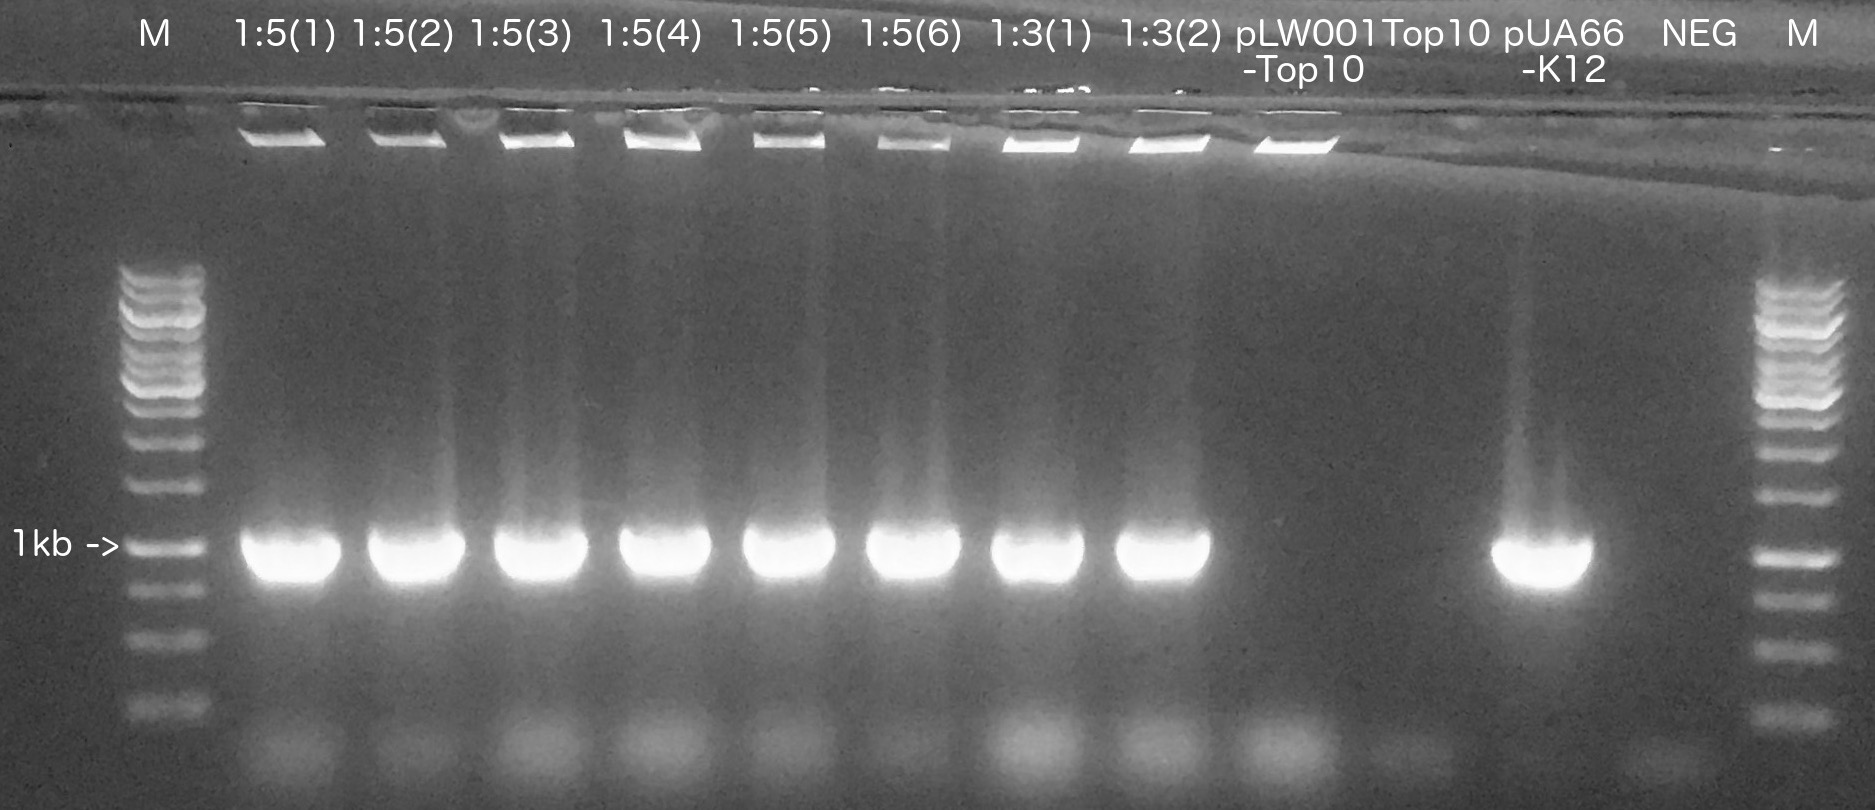
\includegraphics[scale=0.2]{text/Pictures/ColonyPCR.jpg}
	\caption{Electrophoresis of colony PCR using pUA66\textunderscore clon primers; M - marker; first 8 samples (1:5(1) - 1:3(2)) - tested clones; pLW001-Top10 and Top10 - negative controls with template DNA; pUA66-K12 - positive control; NEG - negative control without template DNA.}
	\label{colonyPCR}
\end{figure}
Sanger sequencing confirmed the presence of desired insert in digested pLW001 vector.
However, we identified four SNPs compared to the expected sequence in GFP gene (Fig. \ref{1:3(1)seq}).
But as both sequenced clones have exactly the same SNPs (\hyperlink{pADOUCHseq}{Appendix 7}) and all of these SNPs are synonymous (Fig. \ref{1:3(1)seq}), we inferred that the reference sequence of GFP gene in the pUA66 plasmid was inaccurate.
Complete revised sequence of pADOUCH vector can be found in \hyperlink{pADOUCHwhole}{Appendix 8}.
\begin{figure}[ht]
  \centering
  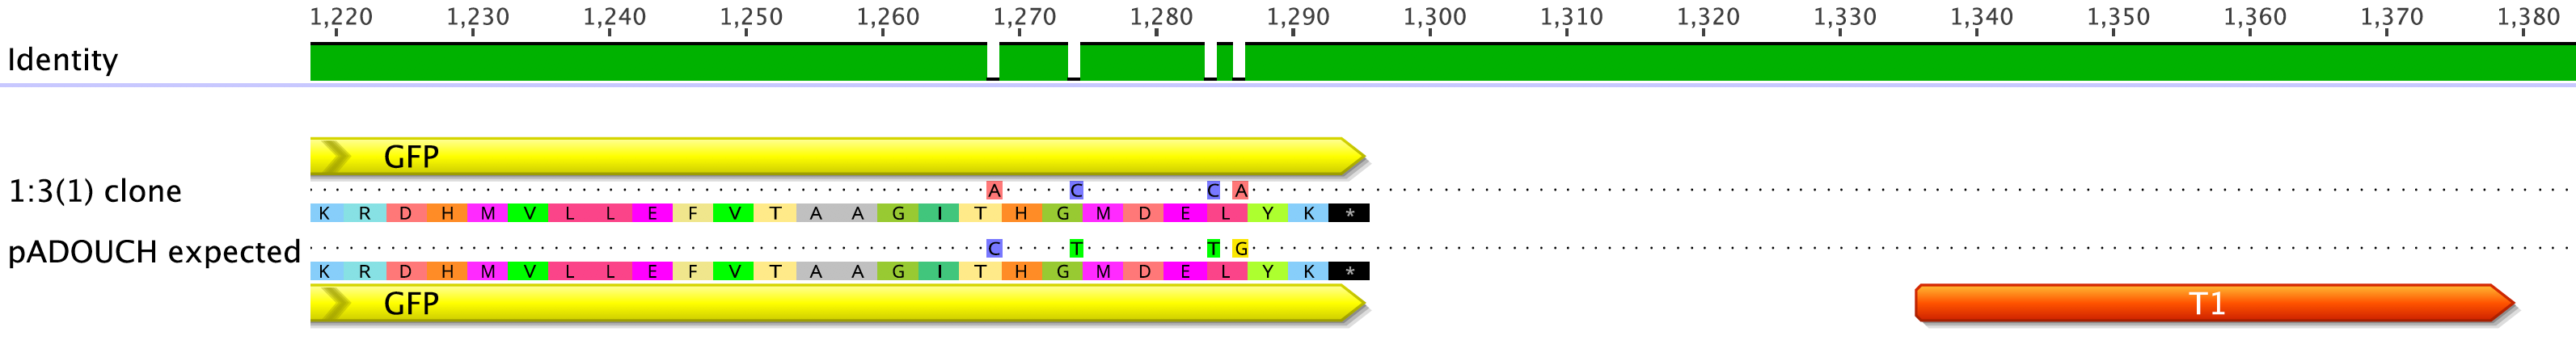
\includegraphics[scale=0.26]{text/Pictures/pADOUCHseq.png}
	\caption{Excerpt of 1:3(1) clone sequence alignment with expected pADOUCH references. DNA sequence is dotted except for SNPs; protein sequence is always beneath its DNA sequence.}
	\label{1:3(1)seq}
\end{figure}

\shorthandon{-} 
%%%%%%%%%%%%%%%%%%%%%%%%%%%%%%%%%%%%




\chapter{Discussion}
%\addcontentsline{toc}{chapter}{Discussion}

\section{Specifita selekce pomocí PCR}
Z celkového počtu 439 presumptivních pseudomonád bylo pomocí PCR amplifikace genu~\tax{rpoD} a~variabilní části genu \tax{rrs} zahrnuto 240 kmenů do užšího výběru, který by~měl zahrnovat pouze zástupce rodu \tax{Pseudomonas}.
Avšak ne u všech izolátů sem~zahrnutých byly jednoznačně produkovány oba amplikony.
V případě 23~kmenů došlo k~pozitivní reakci pouze u~jednoho genu a~to i~v~případě opakovaného procesu.
U~22~zástupců byl detekován jen amplikon pro část genu \tax{rrs} a u jednoho byl přítomen pouze amplikon o~specifické délce genu~\tax{rpoD} s~negativní reakcí pro~\tax{rrs}~gen.
Tudíž tento soubor 240~kmenů teoreticky může zahrnovat i~zástupce mimo rod \tax{Pseudomonas}.

Během optimalizace obou PCR však byla testována specifita použitých primerů s~využitím 25~gramnegativních bakterií mimo~rod \tax{Pseudomonas}.
Níže uvádím Tabulku \ref{kontroly_PCR} s~výsledky reakcí.
PCR pro amplifikaci části genu \tax{rrs}, vytváří amplikon o délce odpovídající specifickému produktu i u kmene \tax{Azotobacter chroococcum} CCM 1912.
Bakterie rodu \tax{Azotobacter} jsou fylogeneticky pseudomonádám velmi blízké, avšak vyžadují pro svůj růst v~laboratorních podmínkách speciální media.
Žádné z těchto medií nebylo použito k~izolaci kmenů, tudíž je prakticky vyloučeno aby se zde tito zástupci vyskytovali.
Přítomnost nepříliš jasného amplikonu u typového kmene \tax{Raoultella terrigena} CCM 3568$^T$ také není velkým problémem.
Žádný z pracovních kmenů totiž není schopen fermentace glukózy, zatímco \tax{R. terrigena} je fakultativně anaerobní druh.
Přesto zjištění, že dané primery tvoří produkty o stejné délce jako specifické amplikony bylo překvapením.
V publikaci, ze~které jsem sekvence primerů čerpala, není o této nespecificitě zmínka. \cite{nair2014molecular}

Podobně i při použití primerů pro amplifikaci genu \tax{rpoD} jsme narazili na dvě falešně pozitivní reakce.
Šlo o 2 druhy aeromonád ze tří porovnávaných.
Tato nespecificita pro~nás ani tentokrát nečiní překážku v~použití primerů k~selekci pseudomonád, jelikož aeromonády jsou schopny fermentace glukózy, kdežto náš soubor již před tříděním obsahoval pouze nefermentující kmeny.
Původní publikace se opět o produkci amplikonů u~aeromonád s~délkou odpovídající specifickým produktům nezmiňuje. \cite{mulet2009rpod}
Avšak je zde poukázáno na možnou nespecificitu ve vztahu k rodu \tax{Alcanivorax} (z~řádu \tax{Oceanospirillales}).
Fenotypem se podobá pseudomonádám.
Má taktéž pouze respiratorní metabolismus, gramnegativní typ buněčné stěny, redukuje nitráty a~vykazuje katalázovou i~oxidázovou aktivitu.
Kolonie jsou bezbarvé. \cite{garrity2005bergey}
Jelikož v~České sbírce mikroorganismů není tento taxon k dispozici, nahradila jsem jej pro~tyto účely fylogeneticky příbuzným typovým kmenem \tax{Halomonas sulfidaeris} CCM 7108$^T$.
K~nespecifické reakci však u tohoto kmene nedošlo.

\begin{center}
\begin{longtable}[c]{|l|l|c|c|}
\caption{Referenční kmeny použité pro kontrolu specifity PCR s výsledky amplifikace} \label{kontroly_PCR} \\

\toprule \multicolumn{1}{|l|}{\textbf{Řád}} & \multicolumn{1}{l|}{\textbf{Referenční kmen}} & \multicolumn{1}{c|}{\textbf{\tax{rrs}}} & \multicolumn{1}{c|}{\textbf{\tax{rpoD}}}\\
\midrule
\endhead

\bottomrule
\endlastfoot

\tax{Rhizobiales} & \tax{Rhizobium radiobacter} CCM 2928 & - & -\\
\hline
\tax{Sphingomonadales} & \tax{Sphingomonas paucimobilis} CCM 3293 & - & -\\
\hline
\multirow{2}{*}{\tax{Burkholderiales}} & \tax{Alcaligenes faecalis} CCM 1052 & - & -\\
& \tax{Burkholderia cepacia} CCM 2656 & - & -\\
\hline
\multirow{3}{*}{\tax{Aeromonadales}} & \tax{Aeromonas dhakensis} CCM 7146 & - & +\\
& \tax{Aeromonas fluvialis} CCM 8437$^T$ & - & -\\
& \tax{Aeromonas hydrophila} CCM 2278 & - & +\\
\hline
\multirow{10}{*}{\tax{Enterobacteriales}} & \tax{Budvicia aquatica} CCM 3714 & - & -\\
& \tax{Citrobacter murliniae} CCM 4834$^T$ & - & -\\
& \tax{Enterobacter cloacae} CCM 1903 & - & -\\
& \tax{Erwinia amylovora} CCM 1114$^T$ & - & -\\
& \tax{Escherichia coli} CCM 5172$^T$ & - & -\\
& \tax{Hafnia alvei} CCM 4845 & - & -\\
& \tax{Klebsiella pneumoniae} CCM 7798$^T$ & - & -\\
& \tax{Rahnella aquatilis} CCM 4086 & - & -\\
& \tax{Raoultella terrigena} CCM 3568$^T$ & w & -\\
& \tax{Tatumella terrea} CCM 4324$^T$ & - & -\\
\hline
\tax{Oceanospirillales} & \tax{Halomonas sulfidaeris} CCM 7108$^T$ & - & -\\
\hline
\multirow{3}{*}{\tax{Pseudomonadales}} & \tax{Acinetobacter bohemicus} CCM 8462$^T$ & - & -\\
& \tax{Azotobacter chroococcum} CCM 1912 & + & -\\
& \tax{Psychrobacter faecalis} CCM 7339$^T$ & - & -\\
\hline
\multirow{2}{*}{\tax{Vibrionales}} & \tax{Vibrio alginolyticus} CCM 3578$^T$ & - & -\\
& \tax{Vibrio metschnikovii} CCM 7098 & - & -\\
\hline
\multirow{2}{*}{\tax{Xanthomonadales}} & \tax{Stenotrophomonas maltophilia} CCM 1640$^T$ & - & -\\
& \tax{Xanthomonas vesicatoria} CCM 2102 & - & -\\
\end{longtable}
\footnotesize
	\emph{Vysvětlivky:} + = pozitivní reakce; - = negativní reakce; w = přítomnost nejasného amplikonu\\*
	\end{center}

I přes zmíněné nespecificity jsme se rozhodli kombinaci těchto primerů použít pro~selekci psudomonád z počátečního souboru suspektních kmenů.
Ve fenotypizaci se nám následně vyčlenila skupina 28 izolátů (\textbf{\textcolor[RGB]{255, 0, 0}{Fenon 1}}), lišících se svými znaky od~hlavního shluku.
Mezi těmito kmeny by se mohly vyskytovat zástupci jiných rodů než \tax{Pseudomonas}.
Nasvědčuje tomu i fakt, že 90\%~zástupců nerostoucích na mS1 agaru, jenž má sloužit k~selekci pseudomonád z~prostředí \cite{gould1985new, tarnawski2003examination} se v~tomto fenonu nachází.
Ten obsahuje též~nadpoloviční většinu zástupců určených pouze jednou pozitivní uniplex~PCR mezi~pseudomonády.
Nicméně následná genotypizace tuto myšlenku nepotvrzuje, jelikož \textbf{\textcolor[RGB]{255, 0, 0}{Fenon 1}} roztříštila do mnoha shluků v celém dendrogramu.
S jistotou však vyloučit přítomnost jiných rodů než \tax{Pseudomonas} v~celém souboru 240~kmenů zatím nelze.

Co se týče falešně negativních výsledků a tedy chybného vyloučení izolátů z pseudomonád, opírám se především o testy citlivosti prováděné v rámci zmiňovaných studií. \cite{mulet2009rpod, nair2014molecular}
Chybovost také snižuje použití dvou rodově specifických reakcí místo jedné.
Tudíž u kmenů s pozitivní pouze jednou PCR se můžeme cíleně zaměřit na potvrzení či vyvrácení jejich příslušnosti k pseudomonádám.



\cleardoublepage


\HeadingConclusion
\chapter*{Summary and future work}
\addcontentsline{toc}{chapter}{Summary}

\shorthandoff{-}
Although much effort and focus have been dedicated to the study of natural selection, a lot still remains unclear in this field.
Recently many studies shown that even in clonal bacterial populations we can see different cell responses to the same stimulus.
This study aims to shed more light on whether the mechanisms leading to such variations within a population with the same genetic background are selected for and if so, whether in order to decrease or increase variability in the particular mechanism (i.e., transcriptional noise, plasticity, response speed, sensitivity, and epigenetic memory).
For this the best known bacterial model organism \tax{E. coli} will be used, however, not so well studied environmental isolates of this species will constitute the crucial part in understanding what role the natural selection plays.
The main objectives of this work are 1. Quantify genotypic and phenotypic variation in promoters among environmental \tax{E. coli} isolates and 2. Compare natural variation in transcriptional responses with a neutral model.

\bigbreak
Result summary of this study in progress:
\begin{enumerate}[font=\bfseries]

    \item \textbf{Quantify genotypic and phenotypic variation in promoters among environmental \tax{E. coli} isolates}
    
    \begin{itemize}
    
        \item well-understood \tax{lacZ} and \tax{recA} promoters were used so far to establish main workflows of this study (i.e., flow cytometry and fluorescent microscopy) on a common lab strain MG1655 and one environmental strain SC1\textunderscore D9
        \item a set of five carbon sources, including lactose, was chosen to study \tax{lacZ} promoter responses both separately and in combination
        \item a range of various sub-lethal Ciprofloxacin concentrations was chosen for \tax{recA} promoter study
        \item differences in SC1\textunderscore D9 and MG1655 \tax{lacZ} promoter sequence lead to differential GFP expression in the used plasmid-based model
        \item \tax{lacZ} promoter activity is affected not only by the sequence itself but by the genetic background of the strain as well
        \item \tax{lacZ} promoter plasmid-based model is sensitive to the non-promoter sequences included as a part of the promoter insert upstream of GFP gene
        \item chromosomal integration of GFP gives different expression patterns in non-lactose environments in the case of \tax{lacZ} promoter experiments
        \item \tax{recA} promoter activity increases with increasing Ciprofloxacin concentration
        \item similarly to \tax{lacZ} promoter, the genetic background plays a role in \tax{recA} promoter activity besides the nucleotide sequence itself
        \item fluorescence values obtained by flow cytometry under the exposure of 4.0 ng/ml of Ciprofloxacin are distorted, probably by cell filamentation
        \item plasmid for chromosomal integration of the \tax{promoter::GFP} sequences was constructed
    
    \end{itemize}

\end{enumerate} 

Summary of future work associated with this study:

\begin{enumerate}

    \item \textbf{Quantify genotypic and phenotypic variation in promoters among environmental \tax{E. coli} isolates}
    
    \begin{itemize}
    
        \item 3 more promoters and sets of conditions to study them under are to be defined
        \item about 10 more strains remain to be selected for further work
        \item \tax{placZ::GFP} sequences are to be integrated into a chromosome of studied strains using constructed pADOUCH plasmid
        \item incorporation of a sequence coding an enzymatic auto-splicing RNA downstream of promoter inserts is being considered to avoid differences in 5' end sequences of GFP gene's mRNAs
        \item consistency in GFP expression triggered by \tax{recA} promoter between plasmid-based model and chromosomal integration is to be checked
        \item software for cell segmentation and tracking in phase contrast and/or fluorescent microscopy images remains to be selected
        \item microfluidics setups and workflows are to be established
        \item occurrence of epigenetic memory in selected promoter networks is to be investigated
            
    \end{itemize}
    
    \item \textbf{Compare natural variation in transcriptional responses with neutral model}
    
    \begin{itemize}
    
        \item libraries of selected promoter variants are to be generated by random mutagenesis
        \item obtained variants of promoters from the libraries are to be cloned into studied strains using a plasmid-based system or chromosomal integration with a fluorescent reporter
        \item variations in generated promoter variants are to be measured among studied strains using flow cytometry
        \item differences in generated promoter variants behaviour are to be investigated under dynamic and fluctuating conditions by fluorescent microscopy and microfluidics
        \item natural promoter variations are to be compared to the values obtained from neutral models determining whether natural selection has acted to increase or decrease transcriptional noise, plasticity, response sensitivity, speed and memory
    
    \end{itemize}

\end{enumerate}

Here I have reviewed the literature relevant to my confirmation proposal and outlined current research gaps this work will help to fill.
In the preliminary work I have shown that the main workflows using flow cytometry and fluorescent microscopy are feasible.
Moreover, we already collected data that give us a new information about the activity of the \tax{lacZ} and \tax{recA} promoters in various conditions and different genetic backgrounds.
This forms the basis of future thesis work.

\cleardoublepage%%% keeps correct headings

\shorthandon{-}


\HeadingAppendix
\chapter*{List of Appendices}

\begin{enumerate}
\item Obrázek \ref{rrs_ML}
\item Obrázek \ref{rpoB_ML}
\item Obrázek \ref{rpoD_ML}
\item \hyperlink{SPARC.1}{Titulní strana sborníku SPARC 2016}
\item \hyperlink{SPARC.55}{Abstrakt z příspěvku v rámci SPARC 2016}
%\item \hyperlink{fenotyp.1}{Shluková analýza fenotypu}
%\item \hyperlink{ordination.1}{Ordinační analýza fenotypu}
%\item \hyperlink{genotyp.1}{Shluková analýza genotypu}
\end{enumerate}

\addcontentsline{toc}{chapter}{Appendix}
%\pageref{mypage}
%\hyperlink{fenotyp.1}{Dendrogram biochemie}
%\includepdf[link, linkname=fenotyp, pages=1, landscape, angle=270, fitpaper]{text_prace/Pictures/anal_vse_ward_jacc_colXYZA.pdf}

%\includepdf[link, linkname=ordination, pages=1, landscape, fitpaper]{text_prace/Pictures/anal_vse_PoCA_jaccard_big1.pdf}

%\includepdf[link, linkname=genotyp, pages=1, landscape, angle=270, fitpaper]{text_prace/Pictures/RPearson-reduction_XYZA_colFULL1.pdf}
\begin{figure}[h!!!]
  \centering
  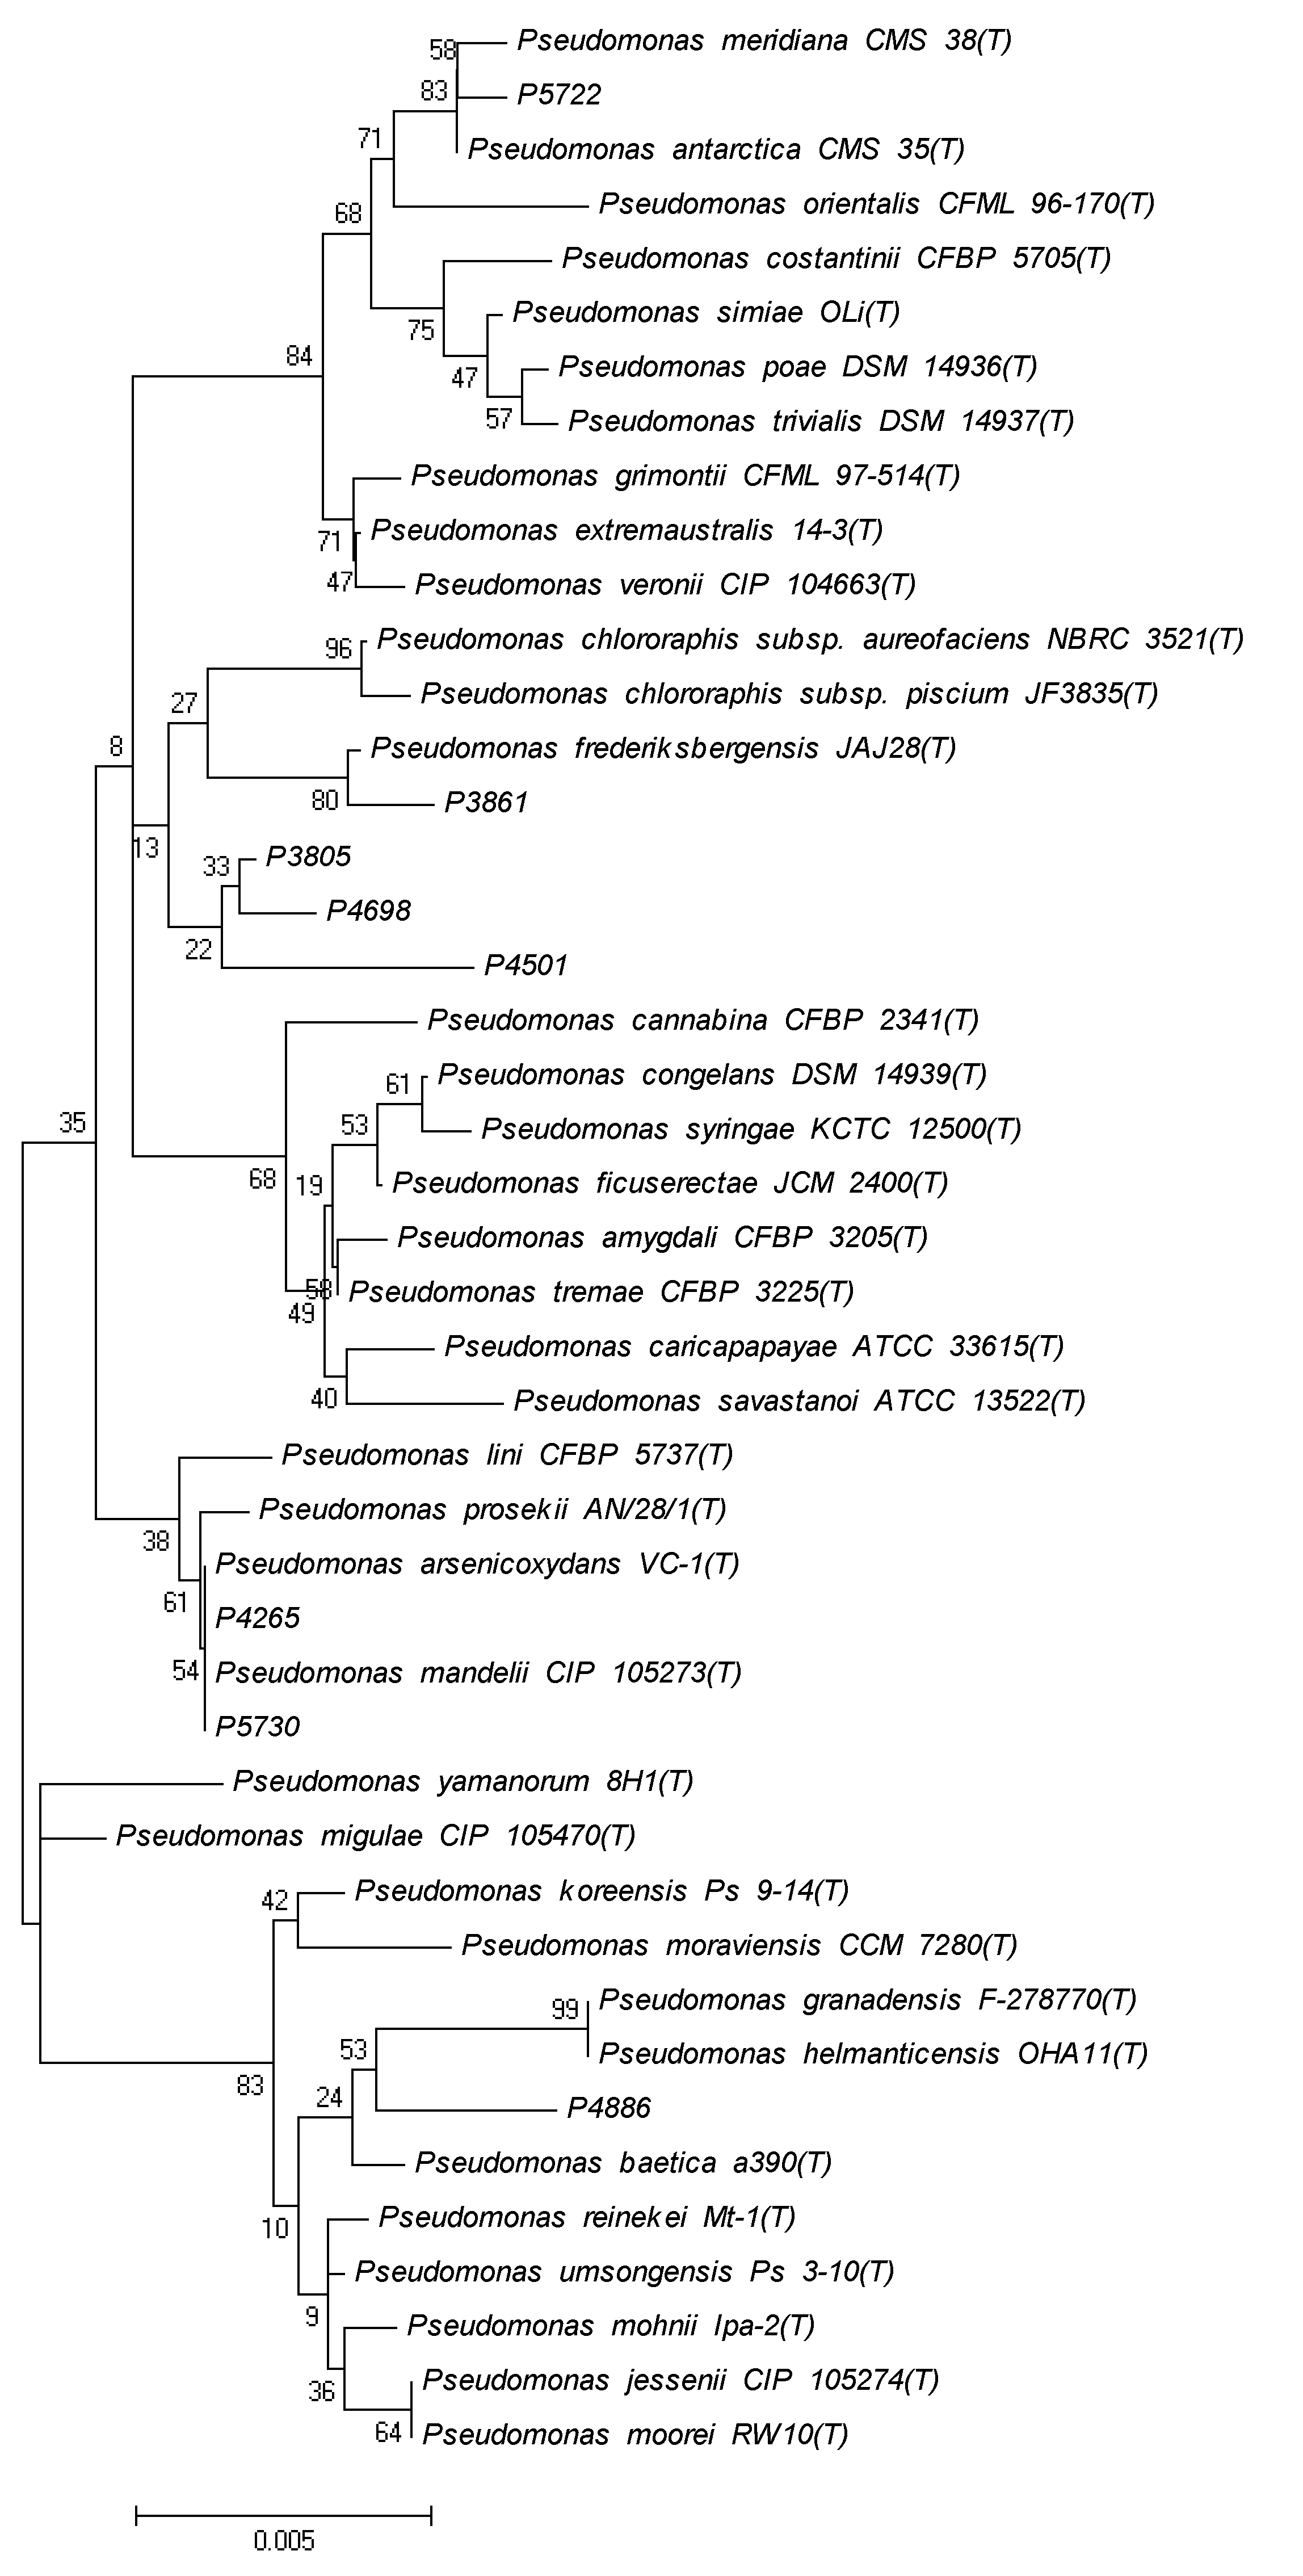
\includegraphics[scale=0.50]{text/Pictures/160508_16S_ML_clustalW_Bootstrap-consensus.png}
	\caption{Fylogenetický strom na základě analýzy genu \tax{rrs} dle metody Maximum-likelihood}
	\label{rrs_ML}
\end{figure}
\pagebreak

\begin{figure}[h!!!]
  \centering
  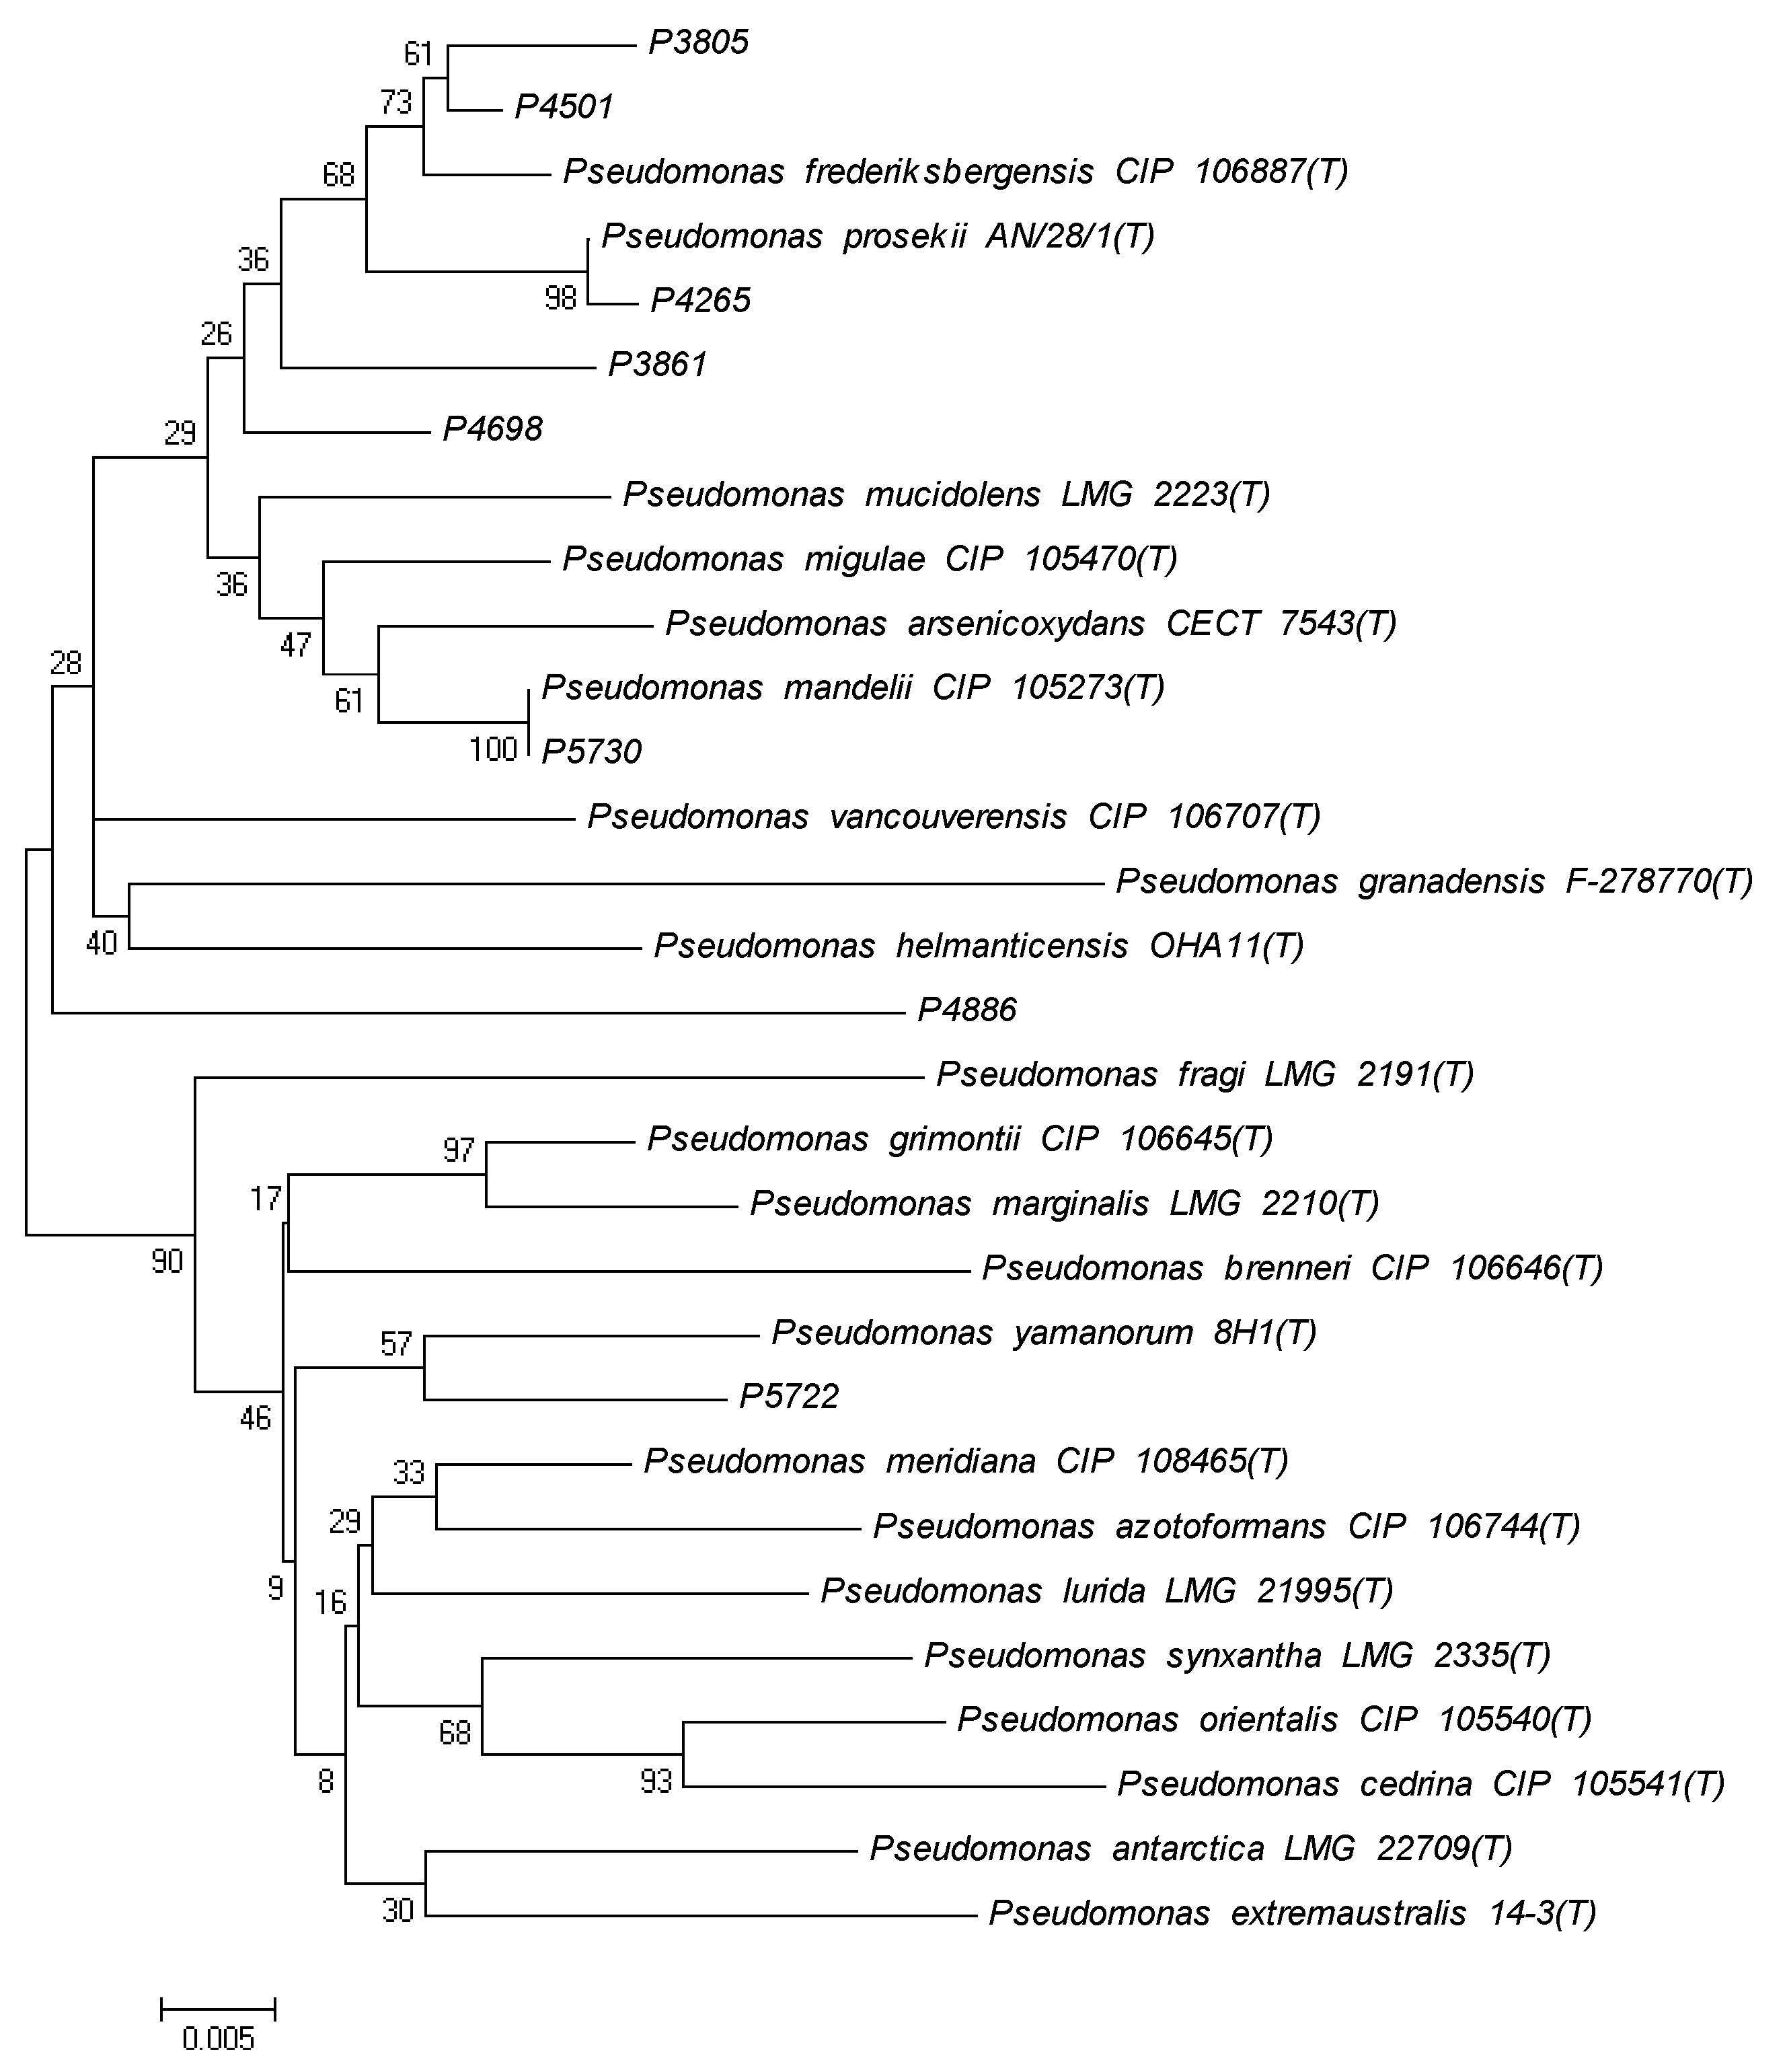
\includegraphics[scale=0.50]{text/Pictures/160508_rpoB_multifasta_doplnek_ML_clustalW_Bootstrap-consensus.png}
	\caption{Fylogenetický strom na základě analýzy genu \tax{rpoB} dle metody Maximum-likelihood}
	\label{rpoB_ML}
\end{figure}
\pagebreak

\begin{figure}[h!!!]
  \centering
  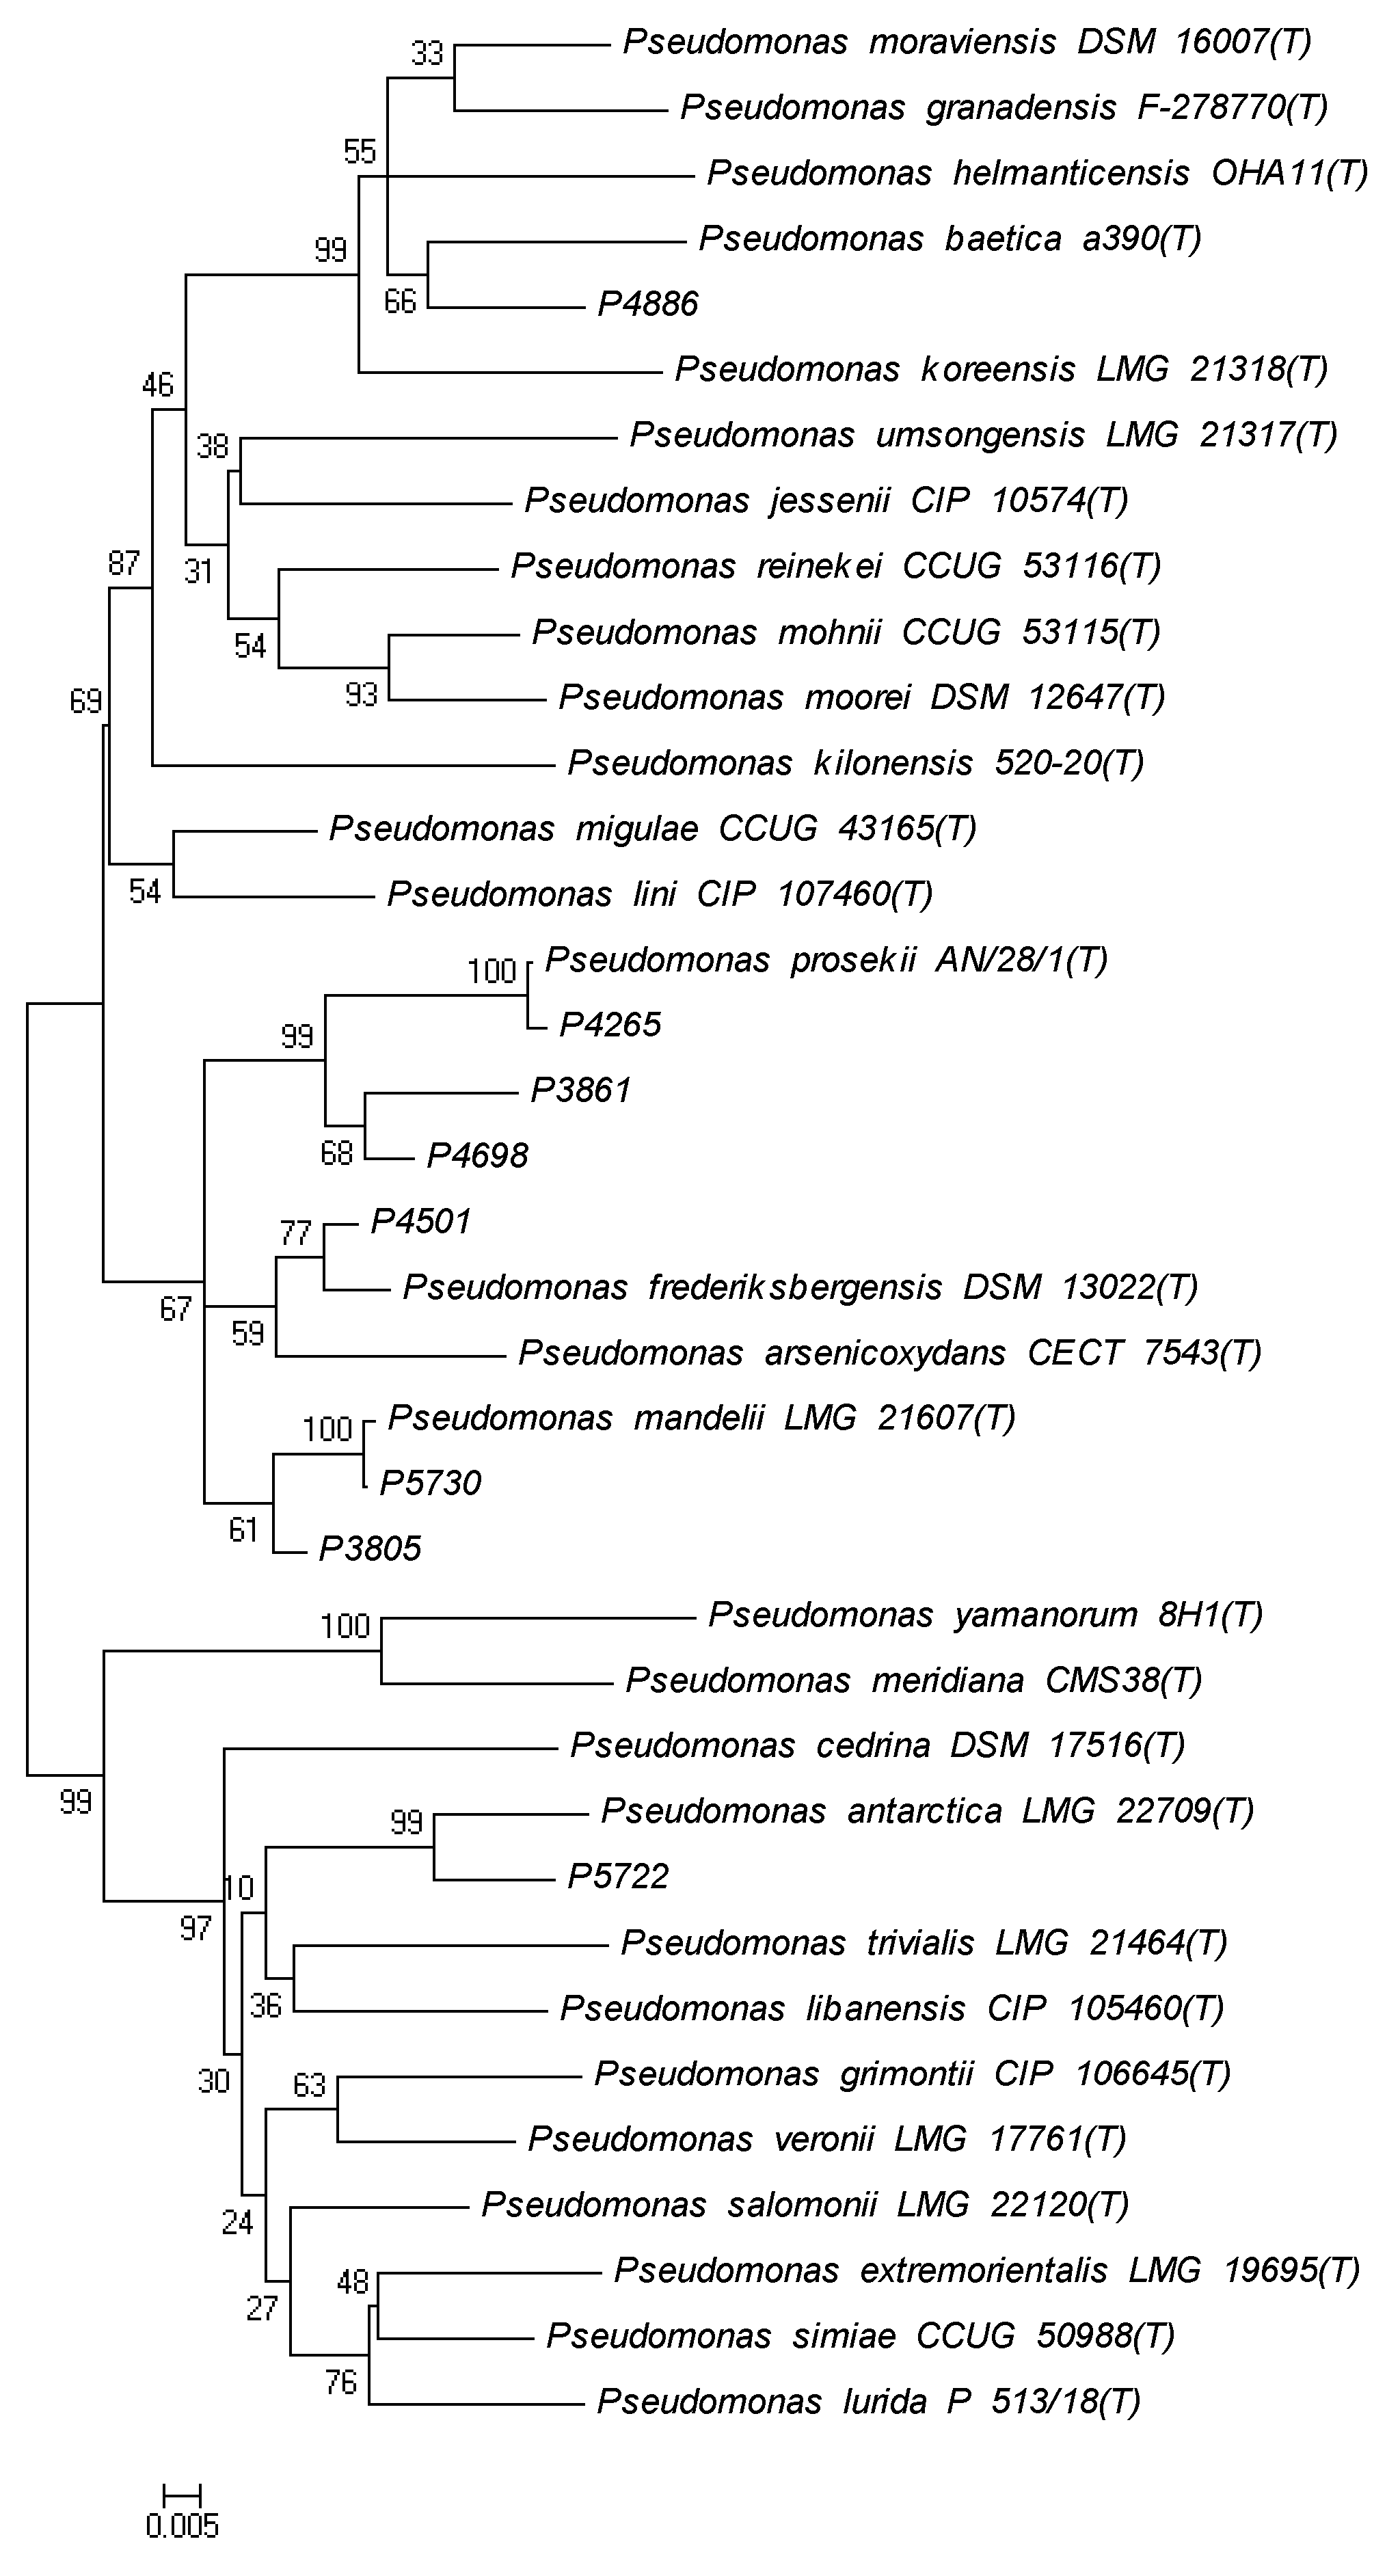
\includegraphics[scale=0.50]{text/Pictures/160508_rpoD_multifasta_doplnek_ML_clustalW_Bootstrap-consensus.png}
	\caption{Fylogenetický strom na základě analýzy genu \tax{rpoD} dle metody Maximum-likelihood}
	\label{rpoD_ML}
\end{figure}
\clearpage

\includepdf[link, linkname=SPARC, pages=1, landscape, fitpaper]{text/Pictures/Sbornik-SPARC2016.pdf}

\includepdf[link, linkname=SPARC, pages=55, landscape, fitpaper]{text/Pictures/Sbornik-SPARC2016.pdf}

%Here is a \hyperlink{anal_vse_ward_jacc_color3.pdf.19}{hyperlink to page 19} of anal_vse_ward_jacc_color3.pdf.

%\medskip

%%%%%%%%%%%%%%%%%%%%%%%%%%%%%%%%%%%%
%%%%%%%%% GENERUJ TEXT %%%%%%%%%%%%%
%%%%%%%%%%%%%%%%%%%%%%%%%%%%%%%%%%%%

\cleardoublepage



\renewcommand{\bibname}{References}
\HeadingLiterature
\addcontentsline{toc}{chapter}{\bibname}

\bibliographystyle{apalike-mv}
\bibliography{Literature}

%%%%%%%%%%%%%%%%%%%%%%%%%%%%%%%%%%%%%%%%%%%%%%%%
%%%%%%%%%%% EMPTY PAGE TO THE END %%%%%%%%%%%%
%%%%%%%%%%%%%%%%%%%%%%%%%%%%%%%%%%%%%%%%%%%%%%%%

\newpage
\thispagestyle{empty}
\fancyhf{}
\newpage
\mbox{}

\end{document}
